%=======================================================================
% riscv-privileged.tex
%-----------------------------------------------------------------------

\documentclass[twoside,11pt]{book}

% Package includes

\usepackage{graphicx}
\usepackage{geometry}
\usepackage{array}
\usepackage{colortbl}
\usepackage[svgnames]{xcolor}

% make links more readable, as they occur often in the op model
%\usepackage{hyperref}
\usepackage[colorlinks,citecolor=DarkGreen,linkcolor=DarkGreen]{hyperref}
\usepackage{placeins}
\usepackage{longtable}
\usepackage{multirow}
\usepackage{float}
\usepackage{listings}
\usepackage{comment}
\usepackage{enumitem}
\usepackage{verbatimbox}

\usepackage[olditem,oldenum]{paralist}

% Setup margins

\setlength{\topmargin}{-0.5in}
\setlength{\textheight}{9in}
\setlength{\oddsidemargin}{0in}
\setlength{\evensidemargin}{0in}
\setlength{\textwidth}{6.5in}

% Useful macros

\newcommand{\note}[1]{{\bf [ NOTE: #1 ]}}
\newcommand{\fixme}[1]{{\bf [ FIXME: #1 ]}}
\newcommand{\todo}[1]{\marginpar{\footnotesize #1}}

\newcommand{\wunits}[2]{\mbox{#1\,#2}}
\newcommand{\um}{\mbox{$\mu$m}}
\newcommand{\xum}[1]{\wunits{#1}{\um}}
\newcommand{\by}[2]{\mbox{#1$\times$#2}}
\newcommand{\byby}[3]{\mbox{#1$\times$#2$\times$#3}}

\newlength\savedwidth
\newcommand\whline[1]{%
  \noalign{%
    \global\savedwidth\arrayrulewidth\global\arrayrulewidth 1.5pt%
  }%
  \cline{#1}%
  \noalign{\vskip\arrayrulewidth}%
  \noalign{\global\arrayrulewidth\savedwidth}%
}

% Custom list environments

\newlist{tightlist}{itemize}{1}
\setlist[tightlist]{label=\textbullet,nosep}

\newenvironment{titledtightlist}[1]
{\noindent
 ~~\textbf{#1}
 \begin{tightlist}}
{\end{tightlist}}

\newenvironment{commentary}
{ \vspace{-0.2in}
  \begin{quotation}
  \noindent
  \small \em
  \rule{\linewidth}{1pt}\\
}
{ 
  \end{quotation}
  \vspace{-0.2in}
}

\newenvironment{samepage-commentary}
{\begin{samepage} \begin{commentary}}
{\end{commentary} \end{samepage}}

\newenvironment{discussion}
{ \vspace{-0.2in}
  \begin{quotation}
  \noindent
  \small \em 
  \rule{\linewidth}{1pt} \\
  {\bf Discussion:}
}
{ 
  \end{quotation}
  \vspace{-0.2in}
}

% Other commands and parameters

\pagestyle{myheadings}
\setlength{\parindent}{0in}
\setlength{\parskip}{10pt}
\sloppy

% Commands for register format figures.

% New column types to use in tabular environment for instruction formats.
% Allocate 0.18in per bit.
\newcolumntype{I}{>{\centering\arraybackslash}p{0.18in}}
% Two-bit centered column.
\newcolumntype{W}{>{\centering\arraybackslash}p{0.36in}}
% Three-bit centered column.
\newcolumntype{F}{>{\centering\arraybackslash}p{0.54in}}
% Four-bit centered column.
\newcolumntype{Y}{>{\centering\arraybackslash}p{0.72in}}
% Five-bit centered column.
\newcolumntype{R}{>{\centering\arraybackslash}p{0.9in}}
% Six-bit centered column.
\newcolumntype{S}{>{\centering\arraybackslash}p{1.08in}}
% Seven-bit centered column.
\newcolumntype{O}{>{\centering\arraybackslash}p{1.26in}}
% Eight-bit centered column.
\newcolumntype{E}{>{\centering\arraybackslash}p{1.44in}}
% Ten-bit centered column.
\newcolumntype{T}{>{\centering\arraybackslash}p{1.8in}}
% Twelve-bit centered column.
\newcolumntype{M}{>{\centering\arraybackslash}p{2.2in}}
% Sixteen-bit centered column.
\newcolumntype{K}{>{\centering\arraybackslash}p{2.88in}}
% Twenty-bit centered column.
\newcolumntype{U}{>{\centering\arraybackslash}p{3.6in}}
% Twenty-bit centered column.
\newcolumntype{L}{>{\centering\arraybackslash}p{3.6in}}
% Twenty-five-bit centered column.
\newcolumntype{J}{>{\centering\arraybackslash}p{4.5in}}

\newcommand{\instbit}[1]{\mbox{\scriptsize #1}}
\newcommand{\instbitrange}[2]{~\instbit{#1} \hfill \instbit{#2}~}
\newcommand{\reglabel}[1]{\hfill {\tt #1}\hfill\ }

\newcommand{\wiri}{\textbf{WIRI}}
\newcommand{\wpri}{\textbf{WPRI}}
\newcommand{\wlrl}{\textbf{WLRL}}
\newcommand{\warl}{\textbf{WARL}}





\newcommand{\privrev}{1.10-draft}

\begin{document}

\title{{\vspace{-0.7in}\Large {\bf The RISC-V Instruction Set Manual}} \\
  \large {\bf Volume II: Privileged Architecture} \\
  Privileged Architecture Version \privrev \\
  Document Version \privrev \\
    {\bf Warning! This draft specification
    will change before being accepted as standard by the RISC-V Foundation, so
    implementations made to this draft specification will likely not conform
    to the future standard.}
  \vspace{-0.1in}}

\author{Editors: Andrew Waterman$^{1}$, Krste Asanovi\'{c}$^{1,2}$ \\
  $^{1}$SiFive Inc., \\
  $^{2}$CS Division, EECS Department, University of California, Berkeley \\
  {\tt andrew@sifive.com, krste@berkeley.edu} \\
  \\
  \parbox{\textwidth}{ Contributors to all versions of the spec in
    alphabetical order (please contact editors to suggest
    corrections): Krste Asanovi\'{c}, Rimas Avi\v{z}ienis, Jacob
    Bachmeyer, Allen J. Baum, Paolo Bonzini, Ruslan Bukin, Christopher
    Celio, David Chisnall, Anthony Coulter,
    Palmer Dabbelt, Monte Dalrymple, Dennis Ferguson,
    Mike Frysinger, John Hauser, David Horner, Olof Johansson, Yunsup Lee,
    Andrew Lutomirski, Jonathan Neusch{\"a}fer, Rishiyur Nikhil,
    Stefan O'Rear, Albert Ou, John Ousterhout, David Patterson, Colin
    Schmidt, Wesley Terpstra, Matt Thomas, Tommy Thorn, Ray
    VanDeWalker, Megan Wachs, Andrew Waterman, and Reinoud Zandijk.}
  \\ \\
  \parbox{\textwidth}{
  This document is released under a Creative Commons Attribution 4.0
  International License.
  }
  \\
  \\
  \parbox{\textwidth}{
    This document is a derivative of the RISC-V
    privileged specification version 1.9.1 released under following license:
    \copyright \,2010--2017 Andrew Waterman, Yunsup Lee, Rimas
    Avi\v{z}ienis, David Patterson, Krste Asanovi\'{c}. 
    Creative Commons Attribution 4.0 International License.
  }
  \\
  \\
  \today
}

\date{} 
\maketitle

\markboth{Volume II: RISC-V Privileged Architectures V\privrev}
{Volume II: RISC-V Privileged Architectures V\privrev}
\thispagestyle{empty}

\frontmatter

\chapter{Preface}

This is version 1.10 of the RISC-V privileged architecture
proposal.  Changes from version 1.9.1 include:

\begin{itemize}
  \parskip 0pt
  \itemsep 1pt
\item The supervisor virtual memory configuration has been moved from the
      {\tt mstatus} register to the {\tt sptbr} register.
\item The SFENCE.VM instruction has been removed in favor of the improved
      SFENCE.VMA instruction.
\item Hardware management of page table entry Accessed and Dirty bits has
      been made optional; simpler implementations may trap to software to
      set them.
\item The counter-enable scheme has changed, so that H-mode and S-mode can
      control availability of counters to S-mode and U-mode, respectively.
\end{itemize}

\section*{Preface to Version 1.9.1}

This is version 1.9.1 of the RISC-V privileged architecture
proposal.  Changes from version 1.9 include:

\begin{itemize}
  \parskip 0pt
  \itemsep 1pt
\item Numerous additions and improvements to the commentary sections.
\item Change configuration string proposal to be use a search process
  that supports various formats including Device Tree String and
  flattened Device Tree.
\item Made {\tt misa} optionally writable to support modifying base
  and supported ISA extensions.  CSR address of {\tt misa} changed.
\item Added description of debug mode and debug CSRs.
\item Added a hardware performance monitoring scheme.  Simplified the
  handling of existing hardware counters, removing privileged versions
  of the counters and the corresponding delta registers.
\item Fixed description of SPIE in presence of user-level interrupts.
\end{itemize}


\tableofcontents

\mainmatter

\chapter{Introduction}

This document describes the RISC-V privileged architecture, which
covers all aspects of RISC-V systems beyond the unprivileged ISA,
including privileged instructions as well as additional functionality
required for running operating systems and attaching external devices.

\begin{commentary}
Commentary on our design decisions is formatted as in this paragraph,
and can be skipped if the reader is only interested in the
specification itself.
\end{commentary}

\begin{commentary}
We briefly note that the entire privileged-level design described in
this document could be replaced with an entirely different
privileged-level design without changing the unprivileged ISA, and
possibly without even changing the ABI.  In particular, this
privileged specification was designed to run existing popular
operating systems, and so embodies the conventional level-based
protection model.  Alternate privileged specifications could embody
other more flexible protection-domain models.  For simplicity of
expression, the text is written as if this was the only possible
privileged architecture.
\end{commentary}

\section{RISC-V Privileged Software Stack Terminology}

This section describes the terminology we use to describe components
of the wide range of possible privileged software stacks for RISC-V.

Figure~\ref{fig:privimps} shows some of the possible software stacks
that can be supported by the RISC-V architecture.  The left-hand side
shows a simple system that supports only a single application running
on an application execution environment (AEE).  The application is
coded to run with a particular application binary interface (ABI).
The ABI includes the supported user-level ISA plus a set of ABI calls to
interact with the AEE.  The ABI hides details of the AEE from the
application to allow greater flexibility in implementing the AEE.  The
same ABI could be implemented natively on multiple different host OSs,
or could be supported by a user-mode emulation environment running on
a machine with a different native ISA.

\begin{figure}[th]
\centering
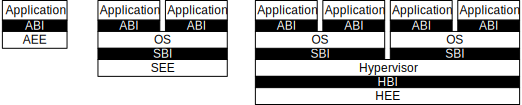
\includegraphics[width=\textwidth]{figs/privimps.pdf}
\caption{Different implementation stacks supporting various forms of
  privileged execution.}
\label{fig:privimps}
\end{figure}

\begin{commentary}
Our graphical convention represents abstract interfaces using black
boxes with white text, to separate them from concrete instances of
components implementing the interfaces.
\end{commentary}

The middle configuration shows a conventional operating system (OS)
that can support multiprogrammed execution of multiple
applications. Each application communicates over an ABI with the OS,
which provides the AEE.  Just as applications interface with an AEE
via an ABI, RISC-V operating systems interface with a supervisor
execution environment (SEE) via a supervisor binary interface (SBI).
An SBI comprises the user-level and supervisor-level ISA together with
a set of SBI function calls.  Using a single SBI across all SEE
implementations allows a single OS binary image to run on any SEE.
The SEE can be a simple boot loader and BIOS-style IO system in a
low-end hardware platform, or a hypervisor-provided virtual machine in
a high-end server, or a thin translation layer over a host operating
system in an architecture simulation environment.

\begin{commentary}
Most supervisor-level ISA definitions do not separate the SBI from the
execution environment and/or the hardware platform, complicating
virtualization and bring-up of new hardware platforms.
\end{commentary}

The rightmost configuration shows a virtual machine monitor
configuration where multiple multiprogrammed OSs are supported by a
single hypervisor.  Each OS communicates via an SBI with the
hypervisor, which provides the SEE.  The hypervisor communicates with
the hypervisor execution environment (HEE) using a hypervisor binary
interface (HBI), to isolate the hypervisor from details of the
hardware platform.

\begin{commentary}
The ABI, SBI, and HBI are still a work-in-progress, but we are now
prioritizing support for Type-2 hypervisors where the SBI is provided
recursively by an S-mode OS.
\end{commentary}

Hardware implementations of the RISC-V ISA will generally require
additional features beyond the privileged ISA to support the various
execution environments (AEE, SEE, or HEE).

\section{Privilege Levels}

At any time, a RISC-V hardware thread ({\em hart}) is running at some
privilege level encoded as a mode in one or more CSRs (control and
status registers).  Three RISC-V privilege levels are currently defined
as shown in Table~\ref{privlevels}.

\begin{table*}[h!]
\begin{center}
\begin{tabular}{|c|c|c|c|}
  \hline
   Level & Encoding & Name      & Abbreviation \\ \hline  
   0     & \tt 00   & User/Application & U     \\ 
   1     & \tt 01   & Supervisor & S           \\ 
   2     & \tt 10   & {\em Reserved} &            \\ 
   3     & \tt 11   & Machine    & M           \\ 
  \hline
 \end{tabular}
\end{center}
\caption{RISC-V privilege levels.}
\label{privlevels}
\end{table*}

Privilege levels are used to provide protection between different
components of the software stack, and attempts to perform operations
not permitted by the current privilege mode will cause an exception to
be raised.  These exceptions will normally cause traps into an
underlying execution environment.

\begin{commentary}
In the description, we try to separate the privilege level for which
code is written, from the privilege mode in which it runs, although
the two are often tied.  For example, a supervisor-level operating
system can run in supervisor-mode on a system with three privilege
modes, but can also run in user-mode under a classic virtual machine
monitor on systems with two or more privilege modes.  In both cases,
the same supervisor-level operating system binary code can be used,
coded to a supervisor-level SBI and hence expecting to be able to use
supervisor-level privileged instructions and CSRs.  When running a
guest OS in user mode, all supervisor-level actions will be trapped
and emulated by the SEE running in the higher-privilege level.
\end{commentary}

The machine level has the highest privileges and is the only mandatory
privilege level for a RISC-V hardware platform.  Code run in
machine-mode (M-mode) is usually inherently trusted, as it has
low-level access to the machine implementation.  M-mode can be used to
manage secure execution environments on RISC-V.  User-mode (U-mode)
and supervisor-mode (S-mode) are intended for conventional application
and operating system usage respectively.

Each privilege level has a core set of privileged ISA extensions with optional
extensions and variants.  For example, machine-mode supports an optional
standard extension for memory protection.  Also, supervisor mode can be
extended to support Type-2 hypervisor execution as described in
Chapter~\ref{hypervisor}.

Implementations might provide anywhere from 1 to 3 privilege modes
trading off reduced isolation for lower implementation cost, as shown
in Table~\ref{privcombs}.

\begin{table*}[h!]
\begin{center}
\begin{tabular}{|c|l|l|}
  \hline
   Number of levels &  Supported Modes & Intended Usage \\ \hline  
   1     & M          & Simple embedded systems \\ 
   2     & M, U       & Secure embedded systems \\ 
   3     & M, S, U    & Systems running Unix-like operating systems\\ 
  \hline
 \end{tabular}
\end{center}
\caption{Supported combinations of privilege modes.}
\label{privcombs}
\end{table*}

All hardware implementations must provide M-mode, as this is the only
mode that has unfettered access to the whole machine.  The simplest
RISC-V implementations may provide only M-mode, though this will
provide no protection against incorrect or malicious application code.

\begin{commentary}
  The lock feature of the optional PMP facility can provide some
  limited protection even with only M-mode implemented.
\end{commentary}

Many RISC-V implementations will also support at least user mode
(U-mode) to protect the rest of the system from application code.
Supervisor mode (S-mode) can be added to provide isolation between a
supervisor-level operating system and the SEE.

A hart normally runs application code in U-mode until some trap (e.g.,
a supervisor call or a timer interrupt) forces a switch to a trap
handler, which usually runs in a more privileged mode. The hart will
then execute the trap handler, which will eventually resume execution
at or after the original trapped instruction in U-mode.  Traps that
increase privilege level are termed {\em vertical} traps, while traps
that remain at the same privilege level are termed {\em horizontal}
traps.  The RISC-V privileged architecture provides flexible routing
of traps to different privilege layers.

\begin{commentary}
Horizontal traps can be implemented as vertical traps that
return control to a horizontal trap handler in the less-privileged mode.
\end{commentary}

\section{Debug Mode}

Implementations may also include a debug mode to support off-chip
debugging and/or manufacturing test.  Debug mode (D-mode) can be
considered an additional privilege mode, with even more access than
M-mode. The separate debug specification proposal describes operation
of a RISC-V hart in debug mode.  Debug mode reserves a few CSR
addresses that are only accessible in D-mode, and may also reserve
some portions of the physical address space on a platform.

\chapter{Control and Status Registers (CSRs)}

The SYSTEM major opcode is used to encode all privileged instructions
in the RISC-V ISA.  These can be divided into two main classes: those
that atomically read-modify-write control and status registers (CSRs),
and all other privileged instructions.  In addition to the user-level
state described in Volume I of this manual, an implementation may
contain additional CSRs, accessible by some subset of the privilege
levels using the CSR instructions described in the user-level manual.
In this chapter, we map out the CSR address space.  The following
chapters describe the function of each of the CSRs according to
privilege level, as well as the other privileged instructions which
are generally closely associated with a particular privilege level.
Note that although CSRs and instructions are associated with one
privilege level, they are also accessible at all higher privilege
levels.

\section{CSR Address Mapping Conventions}

The standard RISC-V ISA sets aside a 12-bit encoding space (csr[11:0])
for up to 4,096 CSRs.  By convention, the upper 4 bits of the CSR
address (csr[11:8]) are used to encode the read and write
accessibility of the CSRs according to privilege level as shown in
Table~\ref{csrrwpriv}.  The top two bits (csr[11:10]) indicate whether
the register is read/write ({\tt 00}, {\tt 01}, or {\tt 10}) or
read-only ({\tt 11}).  The next two bits (csr[9:8]) encode the lowest
privilege level that can access the CSR.

\begin{commentary}
The CSR address convention uses the upper bits of the CSR address to
encode default access privileges.  This simplifies error checking in
the hardware and provides a larger CSR space, but does constrain the
mapping of CSRs into the address space.

Implementations might allow a more-privileged level to trap otherwise
permitted CSR accesses by a less-privileged level to allow these
accesses to be intercepted.  This change should be transparent to the
less-privileged software.
\end{commentary}

\vspace{0.2in}
\begin{table*}[h!]
\begin{center}
\begin{tabular}{|c|c|c|c|l|}
\hline
\multicolumn{3}{|c|}{CSR Address} & Hex & \multicolumn{1}{c|}{Use and Accessibility}\\ \cline{1-3}
[11:10] & [9:8] & [7:6]                  &  & \\
\hline
\multicolumn{5}{|c|}{User CSRs}  \\
\hline
\tt   00   &\tt   00  &\tt   XX     & \tt 0x000-0x0FF & Standard read/write \\ 
\tt   01   &\tt   00  &\tt   XX     & \tt 0x400-0x4FF & Standard read/write \\ 
\tt   10   &\tt   00  &\tt   XX     & \tt 0x800-0x8FF & Non-standard read/write \\ 
\tt   11   &\tt   00  &\tt   00-10  & \tt 0xC00-0xCBF & Standard read-only \\
\tt   11   &\tt   00  &\tt   11     & \tt 0xCC0-0xCFF & Non-standard read-only \\
\hline
\multicolumn{5}{|c|}{Supervisor CSRs}  \\
\hline                                         
\tt   00   &\tt   01  &\tt   XX     & \tt 0x100-0x1FF & Standard read/write \\ 
\tt   01   &\tt   01  &\tt   00-10  & \tt 0x500-0x5BF & Standard read/write \\ 
\tt   01   &\tt   01  &\tt   11     & \tt 0x5C0-0x5FF & Non-standard read/write \\ 
\tt   10   &\tt   01  &\tt   00-10  & \tt 0x900-0x9BF & Standard read/write \\ 
\tt   10   &\tt   01  &\tt   11     & \tt 0x9C0-0x9FF & Non-standard read/write \\ 
\tt   11   &\tt   01  &\tt   00-10  & \tt 0xD00-0xDBF & Standard read-only \\
\tt   11   &\tt   01  &\tt   11     & \tt 0xDC0-0xDFF & Non-standard read-only \\
\hline
\multicolumn{5}{|c|}{Reserved CSRs} \\
\hline                                         
\tt   XX   &\tt   10  &\tt   XX     & Reserved & \\
%% \multicolumn{5}{|c|}{Hypervisor CSRs} \\
%% \hline                                         
%% \tt   00   &\tt   10  &\tt   XX     & \tt 0x200-0x2FF & Standard read/write \\ 
%% \tt   01   &\tt   10  &\tt   00-10  & \tt 0x600-0x6BF & Standard read/write \\ 
%% \tt   01   &\tt   10  &\tt   11     & \tt 0x6C0-0x6FF & Non-standard read/write \\ 
%% \tt   10   &\tt   10  &\tt   00-10  & \tt 0xA00-0xABF & Standard read/write \\ 
%% \tt   10   &\tt   10  &\tt   11     & \tt 0xAC0-0xAFF & Non-standard read/write \\ 
%% \tt   11   &\tt   10  &\tt   00-10  & \tt 0xE00-0xEBF & Standard read-only \\
%% \tt   11   &\tt   10  &\tt   11     & \tt 0xEC0-0xEFF & Non-standard read-only \\
\hline
\multicolumn{5}{|c|}{Machine CSRs}  \\
\hline                                         
\tt   00   &\tt   11  &\tt   XX     & \tt 0x300-0x3FF & Standard read/write \\ 
\tt   01   &\tt   11  &\tt   00-10  & \tt 0x700-0x79F & Standard read/write \\ 
\tt   01   &\tt   11  &\tt   10     & \tt 0x7A0-0x7AF & Standard read/write debug CSRs  \\ 
\tt   01   &\tt   11  &\tt   10     & \tt 0x7B0-0x7BF & Debug-mode-only CSRs \\
\tt   01   &\tt   11  &\tt   11     & \tt 0x7C0-0x7FF & Non-standard read/write \\ 
\tt   10   &\tt   11  &\tt   00-10  & \tt 0xB00-0xBBF & Standard read/write \\ 
\tt   10   &\tt   11  &\tt   11     & \tt 0xBC0-0xBFF & Non-standard read/write \\ 
\tt   11   &\tt   11  &\tt   00-10  & \tt 0xF00-0xFBF & Standard read-only \\
\tt   11   &\tt   11  &\tt   11     & \tt 0xFC0-0xFFF & Non-standard read-only \\
\hline
\end{tabular}
\end{center}
\caption{Allocation of RISC-V CSR address ranges.}
\label{csrrwpriv}
\end{table*}

Attempts to access a non-existent CSR raise an illegal instruction
exception.  Attempts to access a CSR without appropriate privilege
level or to write a read-only register also raise illegal instruction
exceptions.  A read/write register might also contain some bits that
are read-only, in which case writes to the read-only bits are ignored.

Table~\ref{csrrwpriv} also indicates the convention to allocate CSR
addresses between standard and non-standard uses.  The CSR addresses
reserved for non-standard uses will not be redefined by future
standard extensions.

\begin{commentary}
We have dropped the explicit allocation of CSR space for shadow CSRs
to leave more flexibility for allocated other CSRs. Shadow CSRs can
still be added in the appropriate R/W space.  The counters are the
only shadowed CSRs in the current spec.

Shadows CSRs provide a read-write address via which a higher privilege
level can modify a register that is read-only at a lower privilege
level.  Note that if one privilege level has already allocated a
read/write shadow address, then any higher privilege level can use the
same CSR address for read/write access to the same register.
  
Effective virtualization requires that as many instructions run
natively as possible inside a virtualized environment, while any
privileged accesses trap to the virtual machine
monitor~\cite{goldbergvm}.  CSRs that are read-only at some lower
privilege level are shadowed into separate CSR addresses if they are
made read-write at a higher privilege level.  This avoids trapping
permitted lower-privilege accesses while still causing traps on
illegal accesses.
\end{commentary}

Machine-mode standard read-write CSRs {\tt 0x7A0}--{\tt 0x7BF} are
reserved for use by the debug system.  Implementations should raise
illegal instruction exceptions on machine-mode access to these registers.

\section{CSR Listing}

Tables~\ref{ucsrnames}--\ref{mcsrnames} list the CSRs that have
currently been allocated CSR addresses.  The timers, counters, and
floating-point CSRs are standard user-level CSRs, as well as the
additional user trap registers added by the N extension.  The other
registers are used by privileged code, as described in the following
chapters.  Note that not all registers are required on all
implementations.

\begin{table}[htb!]
\begin{center}
\begin{tabular}{|l|l|l|l|}
\hline
Number    & Privilege & Name & Description \\
\hline
\multicolumn{4}{|c|}{User Trap Setup} \\
\hline
\tt 0x000 & URW  &\tt ustatus    & User status register. \\
\tt 0x004 & URW  &\tt uie        & User interrupt-enable register. \\
\tt 0x005 & URW  &\tt utvec      & User trap handler base address. \\
\hline
\multicolumn{4}{|c|}{User Trap Handling} \\
\hline
\tt 0x040 & URW  &\tt uscratch   & Scratch register for user trap handlers. \\
\tt 0x041 & URW  &\tt uepc       & User exception program counter. \\
\tt 0x042 & URW  &\tt ucause     & User trap cause. \\
\tt 0x043 & URW  &\tt utval      & User bad address or instruction. \\
\tt 0x044 & URW  &\tt uip        & User interrupt pending. \\
\hline
\multicolumn{4}{|c|}{User Floating-Point CSRs} \\
\hline
\tt 0x001 & URW  &\tt fflags     & Floating-Point Accrued Exceptions. \\
\tt 0x002 & URW  &\tt frm        & Floating-Point Dynamic Rounding Mode. \\
\tt 0x003 & URW  &\tt fcsr       & Floating-Point Control and Status
Register ({\tt frm} + {\tt fflags}). \\
\hline
\multicolumn{4}{|c|}{User Counter/Timers} \\
\hline
\tt 0xC00 & URO  &\tt cycle         & Cycle counter for RDCYCLE instruction. \\
\tt 0xC01 & URO  &\tt time          & Timer for RDTIME instruction. \\
\tt 0xC02 & URO  &\tt instret       & Instructions-retired counter for RDINSTRET instruction. \\
\tt 0xC03 & URO  &\tt hpmcounter3   & Performance-monitoring counter. \\
\tt 0xC04 & URO  &\tt hpmcounter4   & Performance-monitoring counter. \\
& & \multicolumn{1}{c|}{\vdots} & \ \\
\tt 0xC1F & URO  &\tt hpmcounter31  & Performance-monitoring counter. \\
\tt 0xC80 & URO  &\tt cycleh        & Upper 32 bits of {\tt cycle}, RV32I only. \\
\tt 0xC81 & URO  &\tt timeh         & Upper 32 bits of {\tt time}, RV32I only. \\
\tt 0xC82 & URO  &\tt instreth      & Upper 32 bits of {\tt instret}, RV32I only. \\
\tt 0xC83 & URO  &\tt hpmcounter3h  & Upper 32 bits of {\tt hpmcounter3}, RV32I only. \\
\tt 0xC84 & URO  &\tt hpmcounter4h  & Upper 32 bits of {\tt hpmcounter4}, RV32I only. \\
& & \multicolumn{1}{c|}{\vdots} & \ \\
\tt 0xC9F & URO  &\tt hpmcounter31h & Upper 32 bits of {\tt hpmcounter31}, RV32I only. \\
\hline
\end{tabular}
\end{center}
\caption{Currently allocated RISC-V user-level CSR addresses.}
\label{ucsrnames}
\end{table}

\begin{table}[htb!]
\begin{center}
\begin{tabular}{|l|l|l|l|}
\hline
Number    & Privilege & Name & Description \\
\hline  
\multicolumn{4}{|c|}{Supervisor Trap Setup} \\
\hline
\tt 0x100 & SRW  &\tt sstatus    & Supervisor status register. \\
\tt 0x102 & SRW  &\tt sedeleg    & Supervisor exception delegation register. \\
\tt 0x103 & SRW  &\tt sideleg    & Supervisor interrupt delegation register. \\
\tt 0x104 & SRW  &\tt sie        & Supervisor interrupt-enable register. \\
\tt 0x105 & SRW  &\tt stvec      & Supervisor trap handler base address. \\
\tt 0x106 & SRW  &\tt scounteren & Supervisor counter enable. \\
\hline
\multicolumn{4}{|c|}{Supervisor Trap Handling} \\
\hline
\tt 0x140 & SRW  &\tt sscratch   & Scratch register for supervisor trap handlers. \\
\tt 0x141 & SRW  &\tt sepc       & Supervisor exception program counter. \\
\tt 0x142 & SRW  &\tt scause     & Supervisor trap cause. \\
\tt 0x143 & SRW  &\tt stval      & Supervisor bad address or instruction. \\
\tt 0x144 & SRW  &\tt sip        & Supervisor interrupt pending. \\
\hline
\multicolumn{4}{|c|}{Supervisor Protection and Translation} \\
\hline
\tt 0x180 & SRW  &\tt satp       & Supervisor address translation and protection. \\
\hline
\end{tabular}
\end{center}
\caption{Currently allocated RISC-V supervisor-level CSR addresses.}
\label{scsrnames}
\end{table}

%% \begin{table}[htb!]
%% \begin{center}
%% \begin{tabular}{|l|l|l|l|}
%% \hline
%% Number    & Privilege & Name & Description \\
%% \hline  
%% \multicolumn{4}{|c|}{Hypervisor Trap Setup} \\
%% \hline
%% \tt 0x200 & HRW  &\tt hstatus    & Hypervisor status register. \\
%% \tt 0x202 & HRW  &\tt hedeleg    & Hypervisor exception delegation register. \\
%% \tt 0x203 & HRW  &\tt hideleg    & Hypervisor interrupt delegation register. \\
%% \tt 0x204 & HRW  &\tt hie        & Hypervisor interrupt-enable register. \\
%% \tt 0x205 & HRW  &\tt htvec      & Hypervisor trap handler base address. \\
%% \tt 0x206 & HRW  &\tt hcounteren & Hypervisor counter enable. \\
%% \hline
%% \multicolumn{4}{|c|}{Hypervisor Trap Handling} \\
%% \hline
%% \tt 0x240 & HRW  &\tt hscratch   & Scratch register for hypervisor trap handlers. \\
%% \tt 0x241 & HRW  &\tt hepc       & Hypervisor exception program counter. \\
%% \tt 0x242 & HRW  &\tt hcause     & Hypervisor trap cause. \\
%% \tt 0x243 & HRW  &\tt htval   & Hypervisor bad address or instruction. \\
%% \tt 0x244 & HRW  &\tt hip        & Hypervisor interrupt pending. \\
%% \hline
%% \multicolumn{4}{|c|}{Hypervisor Protection and Translation} \\
%% \hline
%% \tt 0x28X & TBD & TBD & TBD. \\
%% \hline
%% \end{tabular}
%% \end{center}
%% \caption{Currently allocated RISC-V hypervisor-level CSR addresses.}
%% \label{hcsrnames}
%% \end{table}


\begin{table}[htb!]
\begin{center}
\begin{tabular}{|l|l|l|l|}
\hline
Number    & Privilege & Name & Description \\
\hline  
\multicolumn{4}{|c|}{Machine Information Registers} \\
\hline
\tt 0xF11 & MRO &\tt mvendorid   & Vendor ID. \\
\tt 0xF12 & MRO &\tt marchid     & Architecture ID. \\
\tt 0xF13 & MRO &\tt mimpid      & Implementation ID. \\
\tt 0xF14 & MRO &\tt mhartid     & Hardware thread ID. \\
\hline  
\multicolumn{4}{|c|}{Machine Trap Setup} \\
\hline
\tt 0x300 & MRW  &\tt mstatus    & Machine status register. \\
\tt 0x301 & MRW  &\tt misa       & ISA and extensions \\
\tt 0x302 & MRW  &\tt medeleg    & Machine exception delegation register. \\
\tt 0x303 & MRW  &\tt mideleg    & Machine interrupt delegation register. \\
\tt 0x304 & MRW  &\tt mie        & Machine interrupt-enable register. \\
\tt 0x305 & MRW  &\tt mtvec      & Machine trap-handler base address. \\
\tt 0x306 & MRW  &\tt mcounteren & Machine counter enable. \\
\hline
\multicolumn{4}{|c|}{Machine Trap Handling} \\
\hline
\tt 0x340 & MRW  &\tt mscratch   & Scratch register for machine trap handlers. \\
\tt 0x341 & MRW  &\tt mepc       & Machine exception program counter. \\
\tt 0x342 & MRW  &\tt mcause     & Machine trap cause. \\
\tt 0x343 & MRW  &\tt mtval      & Machine bad address or instruction. \\
\tt 0x344 & MRW  &\tt mip        & Machine interrupt pending. \\
\hline
\multicolumn{4}{|c|}{Machine Protection and Translation} \\
\hline
%\tt 0x380 & MRW  &\tt mbase      & Base register. \\
%\tt 0x381 & MRW  &\tt mbound     & Bound register. \\
%\tt 0x382 & MRW  &\tt mibase     & Instruction base register. \\
%\tt 0x383 & MRW  &\tt mibound    & Instruction bound register. \\
%\tt 0x384 & MRW  &\tt mdbase     & Data base register. \\
%\tt 0x385 & MRW  &\tt mdbound    & Data bound register. \\
\tt 0x3A0 & MRW  &\tt pmpcfg0    & Physical memory protection configuration. \\
\tt 0x3A1 & MRW  &\tt pmpcfg1    & Physical memory protection configuration, RV32 only. \\
\tt 0x3A2 & MRW  &\tt pmpcfg2    & Physical memory protection configuration. \\
\tt 0x3A3 & MRW  &\tt pmpcfg3    & Physical memory protection configuration, RV32 only. \\
\tt 0x3B0 & MRW  &\tt pmpaddr0   & Physical memory protection address register. \\
\tt 0x3B1 & MRW  &\tt pmpaddr1   & Physical memory protection address register. \\
& & \multicolumn{1}{c|}{\vdots} & \ \\
\tt 0x3BF & MRW  &\tt pmpaddr15  & Physical memory protection address register. \\
\hline
\end{tabular}
\end{center}
\caption{Currently allocated RISC-V machine-level CSR addresses.}
\label{mcsrnames}
\end{table}

\begin{table}[htb!]
\begin{center}
\begin{tabular}{|l|l|l|l|}
\hline
Number    & Privilege & Name & Description \\
\hline
\multicolumn{4}{|c|}{Machine Counter/Timers} \\
\hline
\tt 0xB00 & MRW  &\tt mcycle         & Machine cycle counter. \\
\tt 0xB02 & MRW  &\tt minstret       & Machine instructions-retired counter. \\
\tt 0xB03 & MRW  &\tt mhpmcounter3   & Machine performance-monitoring counter. \\
\tt 0xB04 & MRW  &\tt mhpmcounter4   & Machine performance-monitoring counter. \\
& & \multicolumn{1}{c|}{\vdots} & \ \\
\tt 0xB1F & MRW  &\tt mhpmcounter31  & Machine performance-monitoring counter. \\
\tt 0xB80 & MRW  &\tt mcycleh        & Upper 32 bits of {\tt mcycle}, RV32I only. \\
\tt 0xB82 & MRW  &\tt minstreth      & Upper 32 bits of {\tt minstret}, RV32I only. \\
\tt 0xB83 & MRW  &\tt mhpmcounter3h  & Upper 32 bits of {\tt mhpmcounter3}, RV32I only. \\
\tt 0xB84 & MRW  &\tt mhpmcounter4h  & Upper 32 bits of {\tt mhpmcounter4}, RV32I only. \\
& & \multicolumn{1}{c|}{\vdots} & \ \\
\tt 0xB9F & MRW  &\tt mhpmcounter31h & Upper 32 bits of {\tt mhpmcounter31}, RV32I only. \\
\hline  
\multicolumn{4}{|c|}{Machine Counter Setup} \\
\hline
\tt 0x323 & MRW  &\tt mhpmevent3     & Machine performance-monitoring event selector. \\
\tt 0x324 & MRW  &\tt mhpmevent4     & Machine performance-monitoring event selector. \\
& & \multicolumn{1}{c|}{\vdots} & \ \\
\tt 0x33F & MRW  &\tt mhpmevent31    & Machine performance-monitoring event selector. \\
\hline
\multicolumn{4}{|c|}{Debug/Trace Registers (shared with Debug Mode)} \\
\hline
\tt 0x7A0 & MRW &\tt tselect & Debug/Trace trigger register select. \\
\tt 0x7A1 & MRW &\tt tdata1 & First Debug/Trace trigger data register. \\
\tt 0x7A2 & MRW &\tt tdata2 & Second Debug/Trace trigger data register. \\
\tt 0x7A3 & MRW &\tt tdata3 & Third Debug/Trace trigger data register. \\
\hline
\multicolumn{4}{|c|}{Debug Mode Registers } \\
\hline
\tt 0x7B0 & DRW &\tt dcsr & Debug control and status register. \\
\tt 0x7B1 & DRW &\tt dpc & Debug PC. \\
\tt 0x7B2 & DRW &\tt dscratch & Debug scratch register. \\
\hline
\end{tabular}
\end{center}
\caption{Currently allocated RISC-V machine-level CSR addresses.}
\label{mcsrnames}
\end{table}

\clearpage

\section{CSR Field Specifications}


The following definitions and abbreviations are used in specifying the
behavior of fields within the CSRs.

\subsection*{Reserved Writes Preserve Values, Reads Ignore Values (WPRI)}

Some whole read/write fields are reserved for future use.  Software
should ignore the values read from these fields, and should preserve
the values held in these fields when writing values to other fields of
the same register.
For forward compatibility, implementations that do not furnish these fields
must hardwire them to zero.
These fields are labeled \wpri\ in the register descriptions.

\begin{commentary}
To simplify the software model, any backward-compatible future
definition of previously reserved fields within a CSR must cope with
the possibility that a non-atomic read/modify/write sequence is used
to update other fields in the CSR.  Alternatively, the original CSR
definition must specify that subfields can only be updated atomically,
which may require a two-instruction clear bit/set bit sequence in
general that can be problematic if intermediate values are not legal.
\end{commentary}

\subsection*{Write/Read Only Legal Values (WLRL)}

Some read/write CSR fields specify behavior for only a subset of
possible bit encodings, with other bit encodings reserved.  Software
should not write anything other than legal values to such a field, and
should not assume a read will return a legal value unless the last
write was of a legal value, or the register has not been written since
another operation (e.g., reset) set the register to a legal value.
These fields are labeled \wlrl\ in the register descriptions.
 
\begin{commentary}
Hardware implementations need only implement enough state bits to
differentiate between the supported values, but must always return the
complete specified bit-encoding of any supported value when read.
\end{commentary}

Implementations are permitted but not required to raise an illegal
instruction exception if an instruction attempts to write a
non-supported value to a CSR field.  Hardware implementations can
return arbitrary bit patterns on the read of a CSR field when the last
write was of an illegal value, but the value returned should
deterministically depend on the illegal written value.

\subsection*{Write Any Values, Reads Legal Values (WARL)}

Some read/write CSR fields are only defined for a subset of bit
encodings, but allow any value to be written while guaranteeing to
return a legal value whenever read.  Assuming that writing the CSR has
no other side effects, the range of supported values can be determined
by attempting to write a desired setting then reading to see if the
value was retained.  These fields are labeled \warl\ in the register
descriptions.

Implementations will not raise an exception on writes of unsupported
values to an \warl\ field.  Implementations must always
deterministically return the same legal value after a given illegal
value is written.

\section{CSR Width Modulation}

If the width of a CSR is changed (for example, by changing MXLEN or UXLEN, as
described in Section~\ref{xlen-control}), the values of the {\em writable}
fields and bits of the new-width CSR are, unless specified otherwise,
determined from the previous-width CSR as though by this algorithm:

\begin{enumerate}

\item The value of the previous-width CSR is copied to a temporary register of
the same width.

\item For the read-only bits of the previous-width CSR, the bits at the same
positions in the temporary register are set to zeros.

\item The width of the temporary register is changed to the new width. If the
new width $W$ is narrower than the previous width, the least-significant $W$
bits of the temporary register are retained and the more-significant bits are
discarded. If the new width is wider than the previous width, the temporary
register is zero-extended to the wider width.

\item Each writable field of the new-width CSR takes the value of the bits at
the same positions in the temporary register.

\end{enumerate}

Changing the width of a CSR is not a read or write of the CSR and thus
does not trigger any side effects.

\chapter{Machine-Level ISA}
\label{machine}

This chapter describes the machine-level operations available in
machine-mode (M-mode), which is the highest privilege mode in a RISC-V
system.  M-mode is the only mandatory privilege mode in a RISC-V
hardware implementation.  M-mode is used for low-level access to a
hardware platform and is the first mode entered at reset.  M-mode can
also be used to implement features that are too difficult or expensive
to implement in hardware directly.  The RISC-V machine-level ISA
contains a common core that is extended depending on which other
privilege levels are supported and other details of the hardware
implementation.

\section{Machine-Level CSRs}

In addition to the machine-level CSRs described in this section,
M-mode code can access all CSRs at lower privilege levels.

\subsection{Machine ISA Register {\tt misa}}

The {\tt misa} register is an XLEN-bit \warl\ read-write register
reporting the ISA supported by the hart.  This register must be
readable in any implementation, but a value of zero can be returned to
indicate the {\tt misa} register has not been implemented, requiring
that CPU capabilities be determined through a separate non-standard
mechanism.

\begin{figure*}[h!]
{\footnotesize
\begin{center}
\begin{tabular}{c@{}c@{}J}
\instbitrange{XLEN-1}{XLEN-2} &
\instbitrange{XLEN-3}{26} &
\instbitrange{25}{0} \\
\hline
\multicolumn{1}{|c|}{Base (\warl)} &
\multicolumn{1}{c|}{\wiri} &
\multicolumn{1}{c|}{Extensions (\warl)} \\
\hline
2 & XLEN-28 & 26 \\
\end{tabular}
\end{center}
}
\vspace{-0.1in}
\caption{Machine ISA register ({\tt misa}).}
\label{misareg}
\end{figure*}

The Base field encodes the native base integer ISA width as shown in
Table~\ref{misabase}.  The Base field may be writable in
implementations that support multiple base ISA widths.  The Base field
is always set to the widest supported ISA variant at reset.

\begin{table*}[h!]
\begin{center}
\begin{tabular}{|r|l|}
\hline
Value  & Description \\
\hline	 
1   & 32 \\
2   & 64 \\
3   & 128 \\
\hline
\end{tabular}
\end{center}
\caption{Encoding of Base field in {\tt misa}}
\label{misabase}
\end{table*}

\begin{commentary}
The base can be quickly ascertained using branches on the sign of the
returned {\tt misa} value, and possibly a shift left by one and a
second branch on the sign.  These checks can be written in assembly
code without knowing the register width (XLEN) of the machine.
The base width is given by $XLEN=2^{Base+4}$.
\end{commentary}

The Extensions field encodes the presence of the standard extensions,
with a single bit per letter of the alphabet (bit 0 encodes presence
of extension ``A'' , bit 1 encodes presence of extension ``B'',
through to bit 25 which encodes ``Z'').  The ``I'' bit will be set for
RV32I, RV64I, RV128I base ISAs, and the ``E'' bit will be set for
RV32E.  The Extension is a \warl\ field that can contain writable bits
where the implementation allows the supported ISA to be modified.  At
reset, the Extension field should contain the maximal set of supported
extensions, and I should be selected over E if both are available.

The ``G'' bit is used as an escape to allow expansion to a larger
space of standard extension names.
\begin{commentary}
G is used to indicate the combination IMAFD, so is redundant in the
{\tt misa} register, hence we reserve the bit to indicate that
additional standard extensions are present.
\end{commentary}

The ``U'',``S'', and ``H'' bits will be set if there is support for
user, supervisor, and hypervisor privilege modes respectively.

The ``X'' bit will be set if there are any non-standard extensions.

\begin{table*}
\begin{center}
\begin{tabular}{|r|r|l|}
\hline
Bit & Character  & Description \\
\hline	 
  0 & A & Atomic extension \\
  1 & B & {\em Tentatively reserved for Bit operations extension} \\
  2 & C & Compressed extension \\
  3 & D & Double-precision floating-point extension \\
  4 & E & RV32E base ISA \\
  5 & F & Single-precision floating-point extension \\
  6 & G & Additional standard extensions present \\
  7 & H & Hypervisor mode implemented \\
  8 & I & RV32I/64I/128I base ISA \\
  9 & J & {\em Reserved} \\
 10 & K & {\em Reserved} \\
 11 & L & {\em Tentatively reserved for Decimal Floating-Point extension} \\
 12 & M & Integer Multiply/Divide extension \\
 13 & N & User-level interrupts supported \\
 14 & O & {\em Reserved} \\
 15 & P & {\em Tentatively reserved for Packed-SIMD extension} \\
 16 & Q & Quad-precision floating-point extension \\
 17 & R & {\em Reserved} \\
 18 & S & Supervisor mode implemented \\
 19 & T & {\em Tentatively reserved for Transactional Memory extension} \\
 20 & U & User mode implemented \\
 21 & V & {\em Tentatively reserved for Vector extension} \\
 22 & W & {\em Reserved} \\
 23 & X & Non-standard extensions present \\
 24 & Y & {\em Reserved} \\
 25 & Z & {\em Reserved} \\
\hline
\end{tabular}
\end{center}
\caption{Encoding of Extensions field in {\tt misa}.  All bits that are
  reserved for future use must return zero when read.}
\label{misaletters}
\end{table*}


\begin{commentary}
The {\tt misa} register exposes a rudimentary catalog of CPU features
to machine-mode code.  More extensive information can be obtained in
machine mode by probing other machine registers, and examining other
ROM storage in the system as part of the boot process.

We require that lower privilege levels execute environment calls
instead of reading CPU registers to determine features available at
each privilege level. This enables virtualization layers to alter the
ISA observed at any level, and supports a much richer command
interface without burdening hardware designs.
\end{commentary}


\clearpage

\subsection{Machine Vendor ID Register {\tt mvendorid}}

The {\tt mvendorid} CSR is an XLEN-bit read-only register encoding the
manufacturer of the part.  This register must be readable in any
implementation, but a value of 0 can be returned to indicate the field
is not implemented or that this is a non-commercial implementation.

\begin{figure*}[h!]
{\footnotesize
\begin{center}
\begin{tabular}{J}
\instbitrange{XLEN-1}{0} \\
\hline
\multicolumn{1}{|c|}{Vendor} \\
\hline
XLEN \\
\end{tabular}
\end{center}
}
\vspace{-0.1in}
\caption{Vendor ID register ({\tt mvendorid}).}
\label{mvendorreg}
\end{figure*}

\begin{commentary}
Non-zero vendor IDs will be allocated by the RISC-V Foundation to commercial
vendors of RISC-V chips.
\end{commentary}

\subsection{Machine Architecture ID Register {\tt marchid}}

The {\tt marchid} CSR is an XLEN-bit read-only register encoding the
base microarchitecture of the hart.  This register must be readable in
any implementation, but a value of 0 can be returned to indicate the
field is not implemented.  The combination of {\tt mvendorid} and {\tt
  marchid} should uniquely identify the type of hart microarchitecture
that is implemented.

\begin{figure*}[h!]
{\footnotesize
\begin{center}
\begin{tabular}{J}
\instbitrange{XLEN-1}{0} \\
\hline
\multicolumn{1}{|c|}{Architecture ID} \\
\hline
XLEN \\
\end{tabular}
\end{center}
}
\vspace{-0.1in}
\caption{Machine Architecture ID register ({\tt marchid}).}
\label{marchreg}
\end{figure*}

Open-source project architecture IDs are allocated globally by the
RISC-V Foundation, and have non-zero architecture IDs with a zero
most-significant-bit (MSB).  Commercial architecture IDs are allocated
by each commercial vendor independently, but must have the MSB set and
cannot contain zero in the remaining XLEN-1 bits.

\begin{commentary}
The intent is for the architecture ID to represent the
microarchitecture associated with the repo around which development
occurs rather than a particular organization.  Commercial fabrications
of open-source designs should (and might be required by the license
to) retain the original architecture ID.  This will aid in reducing
fragmentation and tool support costs, as well as provide attribution.
Open-source architecture IDs should be administered by the Foundation
and should only be allocated to released, functioning open-source
projects.  Commercial architecture IDs can be managed independently by
any registered vendor but are required to have IDs disjoint from the
open-source architecture IDs (MSB set) to prevent collisions if a
vendor wishes to use both closed-source and open-source
microarchitectures.

The convention adopted within the following Implementation field can
be used to segregate branches of the same architecture design,
including by organization.  The {\tt misa} register also helps
distinguish different variants of a design, as does the configuration
string if present.
\end{commentary}

\subsection{Machine Implementation ID Register {\tt mimpid}}

The {\tt mimpid} CSR provides a unique encoding of the version of the
processor implementation.  This register must be readable in any
implementation, but a value of 0 can be returned to indicate that the
field is not implemented.  The Implementation value should reflect the
design of the RISC-V processor itself and not any surrounding system.

\begin{figure*}[h!]
{\footnotesize
\begin{center}
\begin{tabular}{J}
\instbitrange{XLEN-1}{0} \\
\hline
\multicolumn{1}{|c|}{Implementation}  \\
\hline
XLEN \\
\end{tabular}
\end{center}
}
\vspace{-0.1in}
\caption{Machine Implementation ID register ({\tt mimpid}).}
\label{mimpidreg}
\end{figure*}

\begin{commentary}
The format of this field is left to the provider of the architecture
source code, but will be often be printed by standard tools as a
hexadecimal string without any leading or trailing zeros, so the
Implementation value should be left-justified (i.e., filled in from
most-significant nibble down) with subfields aligned on nibble
boundaries to ease human readability.
\end{commentary}

\subsection{Hart ID Register {\tt mhartid}}

The {\tt mhartid} register is an XLEN-bit read-only register
containing the integer ID of the hardware thread running the code.
This register must be readable in any implementation.  Hart IDs might
not necessarily be numbered contiguously in a multiprocessor system,
but at least one hart must have a hart ID of zero.

\begin{figure*}[h!]
{\footnotesize
\begin{center}
\begin{tabular}{J}
\instbitrange{XLEN-1}{0} \\
\hline
\multicolumn{1}{|c|}{Hart ID}\\
\hline
XLEN \\
\end{tabular}
\end{center}
}
\vspace{-0.1in}
\caption{Hart ID register ({\tt mhartid}).}
\label{mhartidreg}
\end{figure*}


\begin{commentary}
In certain cases, we must ensure exactly one hart runs some code
(e.g., at reset), and so require one hart to have a known hart ID of
zero.

For efficiency, system implementers should aim to reduce the magnitude
of the largest hart ID used in a system.
\end{commentary}

\subsection{Machine Status Register ({\tt mstatus})}

The {\tt mstatus} register is an XLEN-bit read/write register
formatted as shown in Figure~\ref{mstatusreg-rv32} for RV32 and
Figure~\ref{mstatusreg} for RV64 and RV128.  The {\tt mstatus}
register keeps track of and controls the hart's current operating
state.  Restricted views of the {\tt mstatus} register appear as the
{\tt hstatus} and {\tt sstatus} registers in the H and S
privilege-level ISAs respectively.

\begin{figure*}[h!]
{\footnotesize
\begin{center}
\setlength{\tabcolsep}{4pt}
\begin{tabular}{cKcccccc}
\\
\instbit{31} &
\instbitrange{30}{21} &
\instbit{20} &
\instbit{19} &
\instbit{18} &
\instbit{17} &
\instbitrange{16}{15} &
 \\
\hline
\multicolumn{1}{|c|}{SD} &
\multicolumn{1}{c|}{\wpri} &
\multicolumn{1}{c|}{TVM} &
\multicolumn{1}{c|}{MXR} &
\multicolumn{1}{c|}{PUM} &
\multicolumn{1}{c|}{MPRV} &
\multicolumn{1}{c|}{XS[1:0]} &
 \\
\hline
1 & 12 & 1 & 1 & 1 & 1 & 2 & \\
\end{tabular}
\begin{tabular}{ccccccccccccc}
\\
&
\instbitrange{14}{13} &
\instbitrange{12}{11} &
\instbitrange{10}{9} &
\instbit{8} &
\instbit{7} &
\instbit{6} &
\instbit{5} &
\instbit{4} &
\instbit{3} &
\instbit{2} &
\instbit{1} &
\instbit{0} \\
\hline
 &
\multicolumn{1}{|c|}{FS[1:0]} &
\multicolumn{1}{c|}{MPP[1:0]} &
\multicolumn{1}{c|}{HPP[1:0]} &
\multicolumn{1}{c|}{SPP} &
\multicolumn{1}{c|}{MPIE} &
\multicolumn{1}{c|}{HPIE} &
\multicolumn{1}{c|}{SPIE} &
\multicolumn{1}{c|}{UPIE} &
\multicolumn{1}{c|}{MIE} &
\multicolumn{1}{c|}{HIE} &
\multicolumn{1}{c|}{SIE} &
\multicolumn{1}{c|}{UIE} \\
\hline
 & 2 & 2 & 2 & 1 & 1 & 1 & 1 & 1 & 1 & 1 & 1 & 1 \\
\end{tabular}
\end{center}
}
\vspace{-0.1in}
\caption{Machine-mode status register ({\tt mstatus}) for RV32.}
\label{mstatusreg-rv32}
\end{figure*}

\begin{figure*}[h!]
{\footnotesize
\begin{center}
\setlength{\tabcolsep}{4pt}
\begin{tabular}{cSccScccccc}
\\
\instbit{XLEN-1} &
\instbitrange{XLEN-2}{36} &
\instbitrange{35}{34} &
\instbitrange{33}{32} &
\instbitrange{31}{21} &
\instbit{20} &
\instbit{19} &
\instbit{18} &
\instbit{17} &
\instbitrange{16}{15} &
 \\
\hline
\multicolumn{1}{|c|}{SD} &
\multicolumn{1}{c|}{\wpri} &
\multicolumn{1}{c|}{SX} &
\multicolumn{1}{c|}{UX} &
\multicolumn{1}{c|}{\wpri} &
\multicolumn{1}{c|}{TVM} &
\multicolumn{1}{c|}{MXR} &
\multicolumn{1}{c|}{PUM} &
\multicolumn{1}{c|}{MPRV} &
\multicolumn{1}{c|}{XS[1:0]} &
 \\
\hline
1 & XLEN-37 & 2 & 2 & 11 & 1 & 1 & 1 & 1 & 2 & \\
\end{tabular}
\begin{tabular}{ccccccccccccc}
\\
&
\instbitrange{14}{13} &
\instbitrange{12}{11} &
\instbitrange{10}{9} &
\instbit{8} &
\instbit{7} &
\instbit{6} &
\instbit{5} &
\instbit{4} &
\instbit{3} &
\instbit{2} &
\instbit{1} &
\instbit{0} \\
\hline
 &
\multicolumn{1}{|c|}{FS[1:0]} &
\multicolumn{1}{c|}{MPP[1:0]} &
\multicolumn{1}{c|}{HPP[1:0]} &
\multicolumn{1}{c|}{SPP} &
\multicolumn{1}{c|}{MPIE} &
\multicolumn{1}{c|}{HPIE} &
\multicolumn{1}{c|}{SPIE} &
\multicolumn{1}{c|}{UPIE} &
\multicolumn{1}{c|}{MIE} &
\multicolumn{1}{c|}{HIE} &
\multicolumn{1}{c|}{SIE} &
\multicolumn{1}{c|}{UIE} \\
\hline
 & 2 & 2 & 2 & 1 & 1 & 1 & 1 & 1 & 1 & 1 & 1 & 1 \\
\end{tabular}
\end{center}
}
\vspace{-0.1in}
\caption{Machine-mode status register ({\tt mstatus}) for RV64 and RV128.}
\label{mstatusreg}
\end{figure*}


\subsection{Privilege and Global Interrupt-Enable Stack in {\tt mstatus} register}
\label{privstack}

Interrupt-enable bits, MIE, HIE, SIE, and UIE, are provided for each privilege
mode.  These bits are primarily used to guarantee atomicity with respect to
interrupt handlers at the current privilege level.  When a hart is executing
in privilege mode {\em x}, interrupts are enabled when {\em x}\,IE=1.
Interrupts for lower privilege modes are always disabled, whereas interrupts
for higher privilege modes are always enabled.  Higher-privilege-level code
can use separate per-interrupt enable bits to disable selected interrupts
before ceding control to a lower privilege level.

\begin{commentary}
The {\em x}IE bits are located in the low-order bits of {\tt mstatus},
allowing them to be atomically set or cleared with a single CSR instruction.
\end{commentary}

To support nested traps, each privilege mode {\em x} has a two-level
stack of interrupt-enable bits and privilege modes.  {\em x}\,PIE
holds the value of the interrupt-enable bit active prior to the trap,
and {\em x}\,PP holds the previous privilege mode.  The {\em x}\,PP
fields can only hold privilege modes up to {\em x}, so MPP and HPP are
two bits wide, SPP is one bit wide, and UPP is implicitly zero.  When
a trap is taken from privilege mode {\em y} into privilege mode {\em
  x}, {\em x}\,PIE is set to the value of {\em y}\,IE; {\em x}\,IE is set to
0; and {\em x}\,PP is set to {\em y}.

\begin{commentary}
For lower privilege modes, any trap (synchronous or asynchronous) is
usually taken at a higher privilege mode with interrupts disabled.
The higher-level trap handler will either service the trap and return
using the stacked information, or, if not returning immediately to the
interrupted context, will save the privilege stack before re-enabling
interrupts, so only one entry per stack is required.
\end{commentary}

The MRET, HRET, SRET, or URET instructions are used to return from
traps in M-mode, H-mode, S-mode, or U-mode respectively.  When
executing an {\em x}RET instruction, supposing {\em x}\,PP holds the
value {\em y}, {\em y}\,IE is set to {\em x}\,PIE; the privilege mode
is changed to {\em y}; {\em x}\,PIE is set to 1; and {\em x}\,PP is
set to U (or M if user-mode is not supported).

\begin{commentary}
When the stack is popped, the lowest-supported privilege mode with
interrupts enabled is added to the bottom of stack to help catch
errors that cause invalid entries to be popped off the stack.
\end{commentary}

{\em x}\,PP fields are \wlrl\ fields that need only be able to store
supported privilege modes.

\begin{commentary}
If the machine provides only U and M modes, then only a single
hardware storage bit is required to represent either 00 or 11 in MPP.
If the machine provides only M mode, then MPP is hardwired to 11.
\end{commentary}

User-level interrupts are an optional extension and have been
allocated the ISA extension letter N.
If user-level interrupts are omitted, the
UIE and UPIE bits are hardwired to zero.  For all other supported
privilege modes {\em x}, the {\em x}\,IE, {\em x}\,PIE, and {\em
  x}\,PP fields are required to be implemented.

\begin{commentary}
User-level interrupts are primarily intended to support secure
embedded systems with only M-mode and U-mode present.
\end{commentary}

\subsection{Base ISA Control in {\tt mstatus} Register}

The SX and UX fields control the value of XLEN for S-mode and U-mode,
respectively.  The encoding of these fields is the same as that of the Base
field of {\tt misa}, shown in Table~\ref{misabase}.  These fields only exist
for RV64 and RV128; RV32 machines always use RV32 for S-mode and U-mode.

The SX field is only implemented if S-mode is implemented, and is otherwise
hard-wired to zero.  An implementation may limit the values to which SX can be
set.  The allowed values for SX may be a function of the machine XLEN.
Changing the machine XLEN (such as by changing the Base field of {\tt misa})
may cause SX to change as a side effect, regardless of whether the previous
value of SX would have been compatible with the new machine XLEN.  An
implementation must enforce that SX specifies a width less than or equal to
the machine XLEN.  If the Base field of {\tt misa} is always nonzero, an
implementation may hard-wire SX to be a read-only copy of Base.

The UX field is only implemented if U-mode is implemented, and is otherwise
hard-wired to zero.  If S-mode is not supported, the allowed values for UX may
be a function of the machine XLEN.  Changing the machine XLEN (such as by
changing the Base field of {\tt misa}) may cause UX to change as a side
effect, regardless of whether the previous value of UX would have been
compatible with the new machine XLEN.  An implementation must enforce that UX
specifies a width less than or equal to the machine XLEN.  If the Base field of
{\tt misa} is always nonzero, an implementation may hard-wire UX to be a
read-only copy of Base.

If S-mode is supported, the allowed values for UX may be a function of the
value of field SX.  Changing SX may cause UX to change as a side effect,
regardless of whether the previous value of UX would have been compatible with
the new SX.  When an instruction explicitly writes both SX and UX together
(such as a CSR instruction that writes {\tt mstatus}), the effect is as though
SX is written first, any side effects from changing SX occur, and then UX is
written.  An implementation must enforce that UX is no greater than SX, and
may hard-wire UX to be a read-only copy of SX.

\subsection{Memory Privilege in {\tt mstatus} Register}

The MPRV bit modifies the privilege level at which loads and stores
execute.  When MPRV=0, translation and protection behave as normal.  When
MPRV=1, data memory addresses are translated and protected as though the
current privilege mode were set to MPP.  Instruction address-translation and
protection are unaffected.

The MXR (Make eXecutable Readable) bit modifies the privilege with
which loads access virtual memory.  When MXR=0, only loads from pages
marked readable (R=1 in Figure~\ref{sv32pte}) will succeed.  When
MXR=1, loads from pages marked either readable or executable (R=1 or
X=1) will succeed.

\begin{commentary}
The MPRV and MXR mechanisms were conceived to improve the efficiency of M-mode
routines that emulate missing hardware features, e.g., misaligned loads and
stores.  MPRV obviates the need to perform address translation in software.
MXR allows instruction words to be loaded from pages marked execute-only.

For simplicity, MPRV and MXR are in effect regardless of privilege
mode, but in normal use will only be enabled for short sequences in
machine mode.
\end{commentary}

The PUM (Protect User Memory) bit modifies the privilege with which S-mode
loads, stores, and instruction fetches access virtual memory.  When PUM=0,
translation and protection behave as normal.  When PUM=1, S-mode memory
accesses to pages that are accessible by U-mode (U=1 in Figure~\ref{sv32pte})
will fault.  PUM has no effect when page-based virtual memory is not in
effect.  Note that, while PUM is ordinarily ignored when not executing in
S-mode, it {\em is} in effect when MPRV=1 and MPP=S.

\subsection{Virtualization Support in {\tt mstatus} Register}

The TVM (Trap Virtual Memory) bit supports intercepting
supervisor virtual-memory management operations.  When TVM=1,
attempts to read or write {\tt sptbr} or execute the SFENCE.VMA
instruction while executing in S-mode will raise an illegal instruction
exception.  When TVM=0, these operations are permitted in S-mode.

\begin{commentary}
The TVM mechanism improves virtualization efficiency by permitting guest
operating systems to execute in S-mode, rather than classically virtualizing
them in U-mode.  This approach obviates the need to trap accesses to most
S-mode CSRs.

Trapping {\tt sptbr} accesses and the SFENCE.VMA instruction provides the
hooks necessary to lazily populate shadow page tables.
\end{commentary}

\note{AW: Describe TW bit, or make WFI M-only.}
\begin{commentary}
Trapping the WFI
instruction can trigger a world switch to another guest OS, rather than
wastefully idling in the current guest.
\end{commentary}

\subsection{Extension Context Status in {\tt mstatus} Register}

Supporting substantial extensions is one of the primary goals of
RISC-V, and hence we define a standard interface to allow unchanged
privileged-mode code, particularly a supervisor-level OS, to support
arbitrary user-mode state extensions.

\begin{commentary}
  To date, there are no standard extensions that define additional
  state beyond the floating-point CSR and data registers.
\end{commentary}

The FS[1:0] read/write field and the XS[1:0] read-only field are used
to reduce the cost of context save and restore by setting and tracking
the current state of the floating-point unit and any other user-mode
extensions respectively.  The FS field encodes the status of the
floating-point unit, including the CSR {\tt fcsr} and floating-point
data registers {\tt f0}--{\tt f31}, while the XS field encodes the
status of any additional user-mode extensions and associated state.
These fields can be checked by a context switch routine to quickly
determine whether a state save or restore is required.  If a save or
restore is required, additional instructions and CSRs are typically
required to effect and optimize the process.

\begin{commentary}
  The design anticipates that most context switches will not need to
  save/restore state in either or both of the floating-point unit or
  other extensions, so provides a fast check via the SD bit.
\end{commentary}

The FS and XS fields use the same status encoding as shown in
Table~\ref{fsxsencoding}, with the four possible status values being
Off, Initial, Clean, and Dirty.

\begin{table*}[h!]
\begin{center}
\begin{tabular}{|r|l|l|}
\hline
Status  & FS Meaning & XS Meaning\\
\hline	 
0 & Off     &  All off \\
1 & Initial &  None dirty or clean, some on\\
2 & Clean   &  None dirty, some clean \\
3 & Dirty   &  Some dirty \\
\hline
\end{tabular}
\end{center}
\caption{Encoding of FS[1:0] and XS[1:0] status fields.}
\label{fsxsencoding}
\end{table*}

In systems that do not implement S-mode and do not have a
floating-point unit, the FS field is hardwired to zero.

In systems without additional user extensions requiring new state, the
XS field is hardwired to zero.  Every additional extension with state
has a local status register encoding the equivalent of the XS states.
If there is only a single additional extension, its status can be
directly mirrored in the XS field.  If there is more than one
additional extension, the XS field represents a summary of all
extensions' status as shown in Table~\ref{fsxsencoding}.

\begin{commentary}
The XS field effectively reports the maximum status value across all
user-extension status fields, though individual extensions can use a
different encoding than XS.
\end{commentary}

The SD bit is a read-only bit that summarizes whether either the FS
field or XS field signals the presence of some dirty state that will
require saving extended user context to memory.  If both XS and FS are
hardwired to zero, then SD is also always zero.

When an extension's status is set to Off, any instruction that
attempts to read or write the corresponding state will cause an
exception.  When the status is Initial, the corresponding state should
have an initial constant value.  When the status is Clean, the
corresponding state is potentially different from the initial value,
but matches the last value stored on a context swap.  When the status
is Dirty, the corresponding state has potentially been modified since
the last context save.

During a context save, the responsible privileged code need only write
out the corresponding state if its status is Dirty, and can then reset
the extension's status to Clean.  During a context restore, the
context need only be loaded from memory if the status is Clean (it
should never be Dirty at restore).  If the status is Initial, the
context must be set to an initial constant value on context restore to
avoid a security hole, but this can be done without accessing memory.
For example, the floating-point registers can all be initialized to
the immediate value 0.

The FS and XS fields are read by the privileged code before saving the
context.  The FS field is set directly by privileged code when
resuming a user context, while the XS field is set indirectly by
writing to the status register of the individual extensions.  The
status fields will also be updated during execution of instructions,
regardless of privilege mode.

Extensions to the user-mode ISA often include additional user-mode
state, and this state can be considerably larger than the base integer
registers.  The extensions might only be used for some applications,
or might only be needed for short phases within a single application.
To improve performance, the user-mode extension can define additional
instructions to allow user-mode software to return the unit to an
initial state or even to turn off the unit.

For example, a coprocessor might require to be configured before use
and can be ``unconfigured'' after use.  The unconfigured state would
be represented as the Initial state for context save.  If the same
application remains running between the unconfigure and the next
configure (which would set status to Dirty), there is no need to
actually reinitialize the state at the unconfigure instruction, as all
state is local to the user process, i.e., the Initial state may only
cause the coprocessor state to be initialized to a constant value at
context restore, not at every unconfigure.

Executing a user-mode instruction to disable a unit and place it into
the Off state will cause an illegal instruction exception to be raised
if any subsequent instruction tries to use the unit before it is
turned back on.  A user-mode instruction to turn a unit on must also
ensure the unit's state is properly initialized, as the unit might
have been used by another context meantime.

Changing the setting of FS has no effect on the contents of the floating-point
register state.  In particular, setting FS=Off does not destroy the state, nor
does setting FS=Initial clear the contents.  Other extensions might not
preserve state when set to Off.

Table~\ref{fsxsstates} shows all the possible state transitions for
the FS or XS status bits.  Note that the standard floating-point
extensions do not support user-mode unconfigure or disable/enable
instructions.

\begin{table*}[h!]
\begin{center}
\begin{tabular}{|l|l|l|l|l|}
\hline
\multicolumn{1}{|r|}{Current State} & Off & Initial & Clean & Dirty \\
Action & & & &\\
\hline
\hline
\multicolumn{5}{|c|}{At context save in privileged code}\\
\hline	 
Save state?    & No         & No        & No     & Yes \\
Next state       & Off        & Initial   & Clean  & Clean \\
\hline
\hline
\multicolumn{5}{|c|}{At context restore in privileged code}\\
\hline
Restore state? & No        & Yes, to initial & Yes, from memory   & N/A \\
Next state     & Off       & Initial   & Clean  & N/A \\
\hline
\hline
\multicolumn{5}{|c|}{Execute instruction to read state}\\
\hline
Action?        & Exception & Execute   & Execute & Execute \\
Next state     & Off       & Initial   & Clean  & Dirty \\
\hline
\hline
\multicolumn{5}{|c|}{Execute instruction to modify state, including configuration}\\
\hline
Action?        & Exception & Execute & Execute & Execute \\
Next state     & Off       & Dirty   & Dirty  & Dirty \\
\hline
\hline
\multicolumn{5}{|c|}{Execute instruction to unconfigure unit}\\
\hline
Action?        & Exception & Execute & Execute & Execute \\
Next state     & Off       & Initial & Initial & Initial \\
\hline
\hline
\multicolumn{5}{|c|}{Execute instruction to disable unit}\\
\hline
Action?        & Execute   & Execute & Execute & Execute \\
Next state     & Off       & Off     & Off     & Off \\
\hline
\hline
\multicolumn{5}{|c|}{Execute instruction to enable unit}\\
\hline
Action?        & Execute   & Execute & Execute & Execute \\
Next state     & Initial   & Initial & Initial & Initial   \\
\hline
\end{tabular}
\end{center}
\caption{FS and XS state transitions.}
\label{fsxsstates}
\end{table*}

Standard privileged instructions to initialize, save, and restore
extension state are provided to insulate privileged code from details
of the added extension state by treating the state as an opaque
object.

\begin{commentary}
Many coprocessor extensions are only used in limited contexts that
allows software to safely unconfigure or even disable units when done.
This reduces the context-switch overhead of large stateful
coprocessors.

We separate out floating-point state from other extension state, as
when a floating-point unit is present the floating-point registers are
part of the standard calling convention, and so user-mode software
cannot know when it is safe to disable the floating-point unit.
\end{commentary}

The XS field provides a summary of all added extension state, but
additional microarchitectural bits might be maintained in the
extension to further reduce context save and restore overhead.

The SD bit is read-only and is set when either the FS or XS bits
encode a Dirty state (i.e., SD=((FS==11) OR (XS==11))).  This allows
privileged code to quickly determine when no additional context save is
required beyond the integer register set and PC.

The floating-point unit state is always initialized, saved, and
restored using standard instructions (F, D, and/or Q), and privileged
code must be aware of FLEN to determine the appropriate space to
reserve for each {\tt f} register.

In a supervisor-level OS, any additional user-mode state should be
initialized, saved, and restored using SBI calls that treats the
additional context as an opaque object of a fixed maximum size.  The
implementation of the SBI initialize, save, and restore calls might
require additional implementation-dependent privileged instructions to
initialize, save, and restore microarchitectural state inside a
coprocessor.

All privileged modes share a single copy of the FS and XS bits.  In a
system with more than one privileged mode, supervisor mode would
normally use the FS and XS bits directly to record the status with
respect to the supervisor-level saved context.  Other more-privileged
active modes must be more conservative in saving and restoring the
extension state in their corresponding version of the context.

\begin{commentary}
In any reasonable use case, the number of context switches between
user and supervisor level should far outweigh the number of context
switches to other privilege levels.  Note that coprocessors should not
require their context to be saved and restored to service asynchronous
interrupts, unless the interrupt results in a user-level context swap.
\end{commentary}

\subsection{Machine Trap-Vector Base-Address Register ({\tt mtvec})}

The {\tt mtvec} register is an XLEN-bit read/write register that holds
the base address of the M-mode trap vector.

\begin{figure*}[h!]
{\footnotesize
\begin{center}
\begin{tabular}{J@{}F}
\instbitrange{XLEN-1}{2} &
\instbitrange{1}{0} \\
\hline
\multicolumn{1}{|c|}{Trap-Vector Base Address (\warl)} & 
\multicolumn{1}{c|}{0} \\
\hline
XLEN-2 & 2 \\
\end{tabular}
\end{center}
}
\vspace{-0.1in}
\caption{Machine trap-vector base-address register ({\tt mtvec}).}
\label{mtvecreg}
\end{figure*}

The {\tt mtvec} register must always be implemented, but can contain
a hardwired read-only value.  If {\tt mtvec} is writable, the set of values
the register may hold can vary by implementation.  The value in the {\tt
mtvec} register must always be aligned on a 4-byte boundary (the low two bits
are always zero).  The value returned by reading a variable {\tt mtvec}
register should always match the value used to generate the handler PC address
when handling traps.

\begin{commentary}
We allow for considerable flexibility in implementation of the trap
vector base address.  On the one hand, we do not wish to burden low-end
implementations with a large number of state bits, but on the other
hand, we wish to allow flexibility for larger systems.
\end{commentary}

By default, all traps into machine mode cause the {\tt pc} to be set to the
value in {\tt mtvec}.  Additional trap vector entry points can be defined by
implementations to allow more rapid identification and service of certain trap
causes.

The location of the reset vector and non-maskable interrupt vector are
implementation-defined.

\begin{commentary}
Reset, NMI vectors, and other interrupt vector default locations are
given in a platform specification.
\end{commentary}

\subsection{Machine Trap Delegation Registers ({\tt medeleg} and {\tt mideleg})}

By default, all traps at any privilege level are handled in machine
mode, though a machine-mode handler can redirect traps back to the
appropriate level with the MRET instruction (Section~\ref{otherpriv}).
To increase performance, implementations can provide individual
read/write bits within {\tt medeleg} and {\tt mideleg} to indicate
that certain exceptions and interrupts should be processed directly by
a lower privilege level.  The machine exception delegation register
({\tt medeleg}) and machine interrupt delegation register ({\tt
  mideleg}) are XLEN-bit read/write registers.

In systems with all four privilege modes (M/H/S/U), a set bit in {\tt
  medeleg} or {\tt mideleg} will delegate any corresponding trap in
U-mode, S-mode, or H-mode to the H-mode trap handler.  H-mode may in
turn set corresponding bits in the {\tt hedeleg} and {\tt hideleg}
registers to delegate traps that occur in S-mode or U-mode to the
S-mode trap handler.  If U-mode traps are supported, S-mode may in
turn set corresponding bits in the {\tt sedeleg} and {\tt sideleg}
registers to delegate traps that occur in U-mode to the U-mode trap
handler.

In systems with three privilege modes (M/S/U), setting a bit in {\tt
  medeleg} or {\tt mideleg} will delegate the corresponding trap in
S-mode or U-mode to the S-mode trap handler. If U-mode traps are
supported, S-mode may in turn set corresponding bits in the {\tt
  sedeleg} and {\tt sideleg} registers to delegate traps that occur in
U-mode to the U-mode trap handler.

In systems with two privilege modes (M/U) and support for U-mode
traps, setting a bit in {\tt medeleg} or {\tt mideleg} will
delegate the corresponding trap in U-mode to the U-mode trap handler.

If systems with only M-mode, or with both M-mode and U-mode but
without U-mode trap support, the {\tt medeleg} and {\tt mideleg}
registers should be hardwired to zero.

When a trap is delegated to a less-privileged mode {\em x}, the
{\em x}\,{\tt cause} register is written with the trap cause; the
{\em x}\,{\tt epc} register is written with the virtual address of
the instruction that took the trap; the {\em x}\,PP field
of {\tt mstatus} is written with the active privilege mode at the time of
the trap; the {\em x}\,PIE field of {\tt mstatus} is written with the
value of the active interrupt-enable bit at the time of the trap; and
the {\em x}\,IE field of {\tt mstatus} is cleared.  The {\tt mcause} and
{\tt mepc} registers and the MPP and MPIE fields of {\tt mstatus} are
not written.

An implementation shall not hardwire any delegation bits to one, i.e.,
any trap that can be delegated must support not being delegated.  An
implementation can choose to subset the delegatable traps, with the
supported delegatable bits found by writing one to every bit location,
then reading back the value in {\tt medeleg} or {\tt mideleg} to see
which bit positions hold a one.

Traps never transition from a more-privileged mode to a less-privileged mode.
For example, if M-mode has delegated illegal instruction traps to S-mode, and
M-mode software later executes an illegal instruction, the trap is taken in
M-mode, rather than being delegated to S-mode.  By contrast, traps may be
taken horizontally.  Using the same example, if M-mode has delegated illegal
instruction traps to S-mode, and S-mode software later executes an illegal
instruction, the trap is taken in S-mode.

\begin{figure}[h!]
{\footnotesize
\begin{center}
\begin{tabular}{@{}U}
\instbitrange{XLEN-1}{0} \\
\hline
\multicolumn{1}{|c|}{Synchronous Exceptions (\warl)} \\
\hline
XLEN \\
\end{tabular}
\end{center}
}
\vspace{-0.1in}
\caption{Machine Exception Delegation Register {\tt medeleg}.}
\label{medelegreg}
\end{figure}

{\tt medeleg} has a bit position allocated for every synchronous exception
shown in Table~\ref{mcauses}, with the index of the bit position equal to the
value returned in the {\tt mcause} register (i.e., setting bit 8 allows
user-mode environment calls to be delegated to a lower-privilege trap
handler).

\begin{figure}[h!]
{\footnotesize
\begin{center}
\begin{tabular}{@{}U}
\instbitrange{XLEN-1}{0} \\
\hline
\multicolumn{1}{|c|}{Interrupts (\warl)} \\
\hline
XLEN \\
\end{tabular}
\end{center}
}
\vspace{-0.1in}
\caption{Machine Exception Delegation Register {\tt mideleg}.}
\label{midelegreg}
\end{figure}

{\tt mideleg} holds trap delegation bits for individual interrupts, with the
layout of bits matching those in the {\tt mip} register (i.e., STIP interrupt
delegation control is located in bit 5).

\subsection{Machine Interrupt Registers ({\tt mip} and {\tt mie})}

The {\tt mip} register is an XLEN-bit read/write register containing
information on pending interrupts, while {\tt mie} is the
corresponding XLEN-bit read/write register containing interrupt enable
bits.  Only the bits corresponding to lower-privilege software
interrupts (USIP, SSIP, HSIP) and timer interrupts (UTIP, STIP and
HTIP) in {\tt mip} are writable through this CSR address; the
remaining bits are read-only.

Restricted views of the {\tt mip} and {\tt mie} registers appear as the {\tt
hip}/{\tt hie}, {\tt sip}/{\tt sie}, and {\tt uip}/{\tt uie} registers in
H-mode, S-mode, and U-mode respectively.  If an interrupt is delegated to
privilege mode {\em x} by setting a bit in the {\tt mideleg} register, it
becomes visible in the {\em x}\,{\tt ip} register and is maskable using the {\em
x}\,{\tt ie} register.  Otherwise, the corresponding bits in {\em x}\,{\tt ip}
and {\em x}\,{\tt ie} appear to be hardwired to zero.

\begin{figure*}[h!]
{\footnotesize
\begin{center}
\setlength{\tabcolsep}{4pt}
\begin{tabular}{Scccccccccccc}
\instbitrange{XLEN-1}{12} &
\instbit{11} &
\instbit{10} &
\instbit{9} &
\instbit{8} &
\instbit{7} &
\instbit{6} &
\instbit{5} &
\instbit{4} &
\instbit{3} &
\instbit{2} &
\instbit{1} &
\instbit{0} \\
\hline
\multicolumn{1}{|c|}{\wiri} &
\multicolumn{1}{c|}{MEIP} &
\multicolumn{1}{c|}{HEIP} &
\multicolumn{1}{c|}{SEIP} &
\multicolumn{1}{c|}{UEIP} &
\multicolumn{1}{c|}{MTIP} &
\multicolumn{1}{c|}{HTIP} &
\multicolumn{1}{c|}{STIP} &
\multicolumn{1}{c|}{UTIP} &
\multicolumn{1}{c|}{MSIP} &
\multicolumn{1}{c|}{HSIP} &
\multicolumn{1}{c|}{SSIP} &
\multicolumn{1}{c|}{USIP} \\
\hline
XLEN-12 & 1 & 1 & 1 & 1 & 1 & 1 & 1 & 1 & 1 & 1 & 1 & 1 \\
\end{tabular}
\end{center}
}
\vspace{-0.1in}
\caption{Machine interrupt-pending register ({\tt mip}).}
\label{mipreg}
\end{figure*}

\begin{figure*}[h!]
{\footnotesize
\begin{center}
\setlength{\tabcolsep}{4pt}
\begin{tabular}{Scccccccccccc}
\instbitrange{XLEN-1}{12} &
\instbit{11} &
\instbit{10} &
\instbit{9} &
\instbit{8} &
\instbit{7} &
\instbit{6} &
\instbit{5} &
\instbit{4} &
\instbit{3} &
\instbit{2} &
\instbit{1} &
\instbit{0} \\
\hline
\multicolumn{1}{|c|}{\wpri} &
\multicolumn{1}{c|}{MEIE} &
\multicolumn{1}{c|}{HEIE} &
\multicolumn{1}{c|}{SEIE} &
\multicolumn{1}{c|}{UEIE} &
\multicolumn{1}{c|}{MTIE} &
\multicolumn{1}{c|}{HTIE} &
\multicolumn{1}{c|}{STIE} &
\multicolumn{1}{c|}{UTIE} &
\multicolumn{1}{c|}{MSIE} &
\multicolumn{1}{c|}{HSIE} &
\multicolumn{1}{c|}{SSIE} &
\multicolumn{1}{c|}{USIE} \\
\hline
XLEN-12 & 1 & 1 & 1 & 1 & 1 & 1 & 1 & 1 & 1 & 1 & 1 & 1 \\
\end{tabular}
\end{center}
}
\vspace{-0.1in}
\caption{Machine interrupt-enable register ({\tt mie}).}
\label{miereg}
\end{figure*}

The MTIP, HTIP, STIP, UTIP bits correspond to timer interrupt-pending
bits for machine, hypervisor, supervisor, and user timer interrupts,
respectively.  The MTIP bit is read-only and is cleared by writing to
the memory-mapped machine-mode timer compare register.  The UTIP, STIP
and HTIP bits may be written by M-mode software to deliver timer
interrupts to lower privilege levels.  User, supervisor and hypervisor
software may clear the UTIP, STIP and HTIP bits with calls to the AEE,
SEE, or HEE, respectively.

There is a separate timer interrupt-enable bit, named MTIE, HTIE,
STIE, and UTIE for M-mode, H-mode, S-mode, and U-mode timer interrupts
respectively.

Each lower privilege level has a separate software interrupt-pending
bit (HSIP, SSIP, USIP), which can be both read and written by CSR
accesses from code running on the local hart at the associated or any
higher privilege level. The machine-level MSIP bits are written by
accesses to memory-mapped control registers, which are used by remote
harts to provide machine-mode interprocessor interrupts.
Interprocessor interrupts for lower privilege levels are implemented
through ABI, SBI or HBI calls to the AEE, SEE or HEE respectively,
which might ultimately result in a machine-mode write to the receiving
hart's MSIP bit.  A hart can write its own MSIP bit using the same
memory-mapped control register.

\begin{commentary}
We only allow a hart to directly write its own HSIP, SSIP, or USIP
bits when running in appropriate mode, as other harts might be
virtualized and possibly descheduled by higher privilege levels.  We
rely on ABI, SBI, and HBI calls to provide interprocessor interrupts
for this reason.  Machine-mode harts are not virtualized and can
directly interrupt other harts by setting their MSIP bits, typically
using uncached I/O writes to memory-mapped control registers depending
on the platform specification.
\end{commentary}

The MEIP, HEIP, SEIP, UEIP bits correspond to external
interrupt-pending bits for machine, hypervisor, supervisor, and user
external interrupts, respectively.  These bits are read-only and are
set and cleared by a platform-specific interrupt controller, such as
the standard platform-level interrupt controller specified in
Chapter~\ref{plic}.  There is a separate external interrupt-enable
bit, named MEIE, HEIE, SEIE, and UEIE for M-mode, H-mode, S-mode, and
U-mode external interrupts respectively.

\begin{commentary}
The non-maskable interrupt is not made visible via the {\tt mip}
register as its presence is implicitly known when executing the NMI
trap handler.
\end{commentary}

For all the various interrupt types (software, timer, and external),
if a privilege level is not supported, the associated pending and
interrupt-enable bits are hardwired to zero in the {\tt mip} and {\tt
  mie} registers respectively.  Hence, these are all effectively
\warl\ fields.

\begin{commentary}
Implementations can add additional platform-specific machine-level
interrupt sources to the high bits of these registers, though the
expectation is that most external interrupts will be routed through
the platform interrupt controller and be delivered via MEIP.
\end{commentary}

An interrupt {\em i} will be taken if bit {\em i} is set in both {\tt
  mip} and {\tt mie}, and if interrupts are globally enabled.  By
default, M-mode interrupts are globally enabled if the hart's current
privilege mode is less than M, or if the current privilege mode is M
and the MIE bit in the {\tt mstatus} register is set.  If bit {\em i}
in {\tt mideleg} is set, however, interrupts are considered to be
globally enabled if the hart's current privilege mode equals the
delegated privilege mode (H, S, or U) and that mode's interrupt enable
bit (HIE, SIE or UIE in {\tt mstatus}) is set, or if the current
privilege mode is less than the delegated privilege mode.

Multiple simultaneous interrupts and traps at the same privilege level
are handled in the following decreasing priority order: external
interrupts, software interrupts, timer interrupts, then finally any
synchronous traps.

\subsection{Machine Timer Registers ({\tt mtime} and {\tt mtimecmp})}

Platforms provide a real-time counter, exposed as a memory-mapped
machine-mode register, {\tt mtime}.  {\tt mtime} must run at constant
frequency, and the platform must provide a mechanism for determining
the timebase of {\tt mtime}.

The {\tt mtime} register has a 64-bit precision on all RV32, RV64, and
RV128 systems.  Platforms provide a 64-bit memory-mapped machine-mode
timer compare register ({\tt mtimecmp}), which causes a timer
interrupt to be posted when the {\tt mtime} register contains a value
greater than or equal to the value in the {\tt mtimecmp} register.
The interrupt remains posted until it is cleared by writing the {\tt
  mtimecmp} register.  The interrupt will only be taken if interrupts
are enabled and the MTIE bit is set in the {\tt mie} register.

\begin{figure}[h!]
{\footnotesize
\begin{center}
\begin{tabular}{@{}J}
\instbitrange{63}{0} \\
\hline
\multicolumn{1}{|c|}{\tt mtime} \\
\hline
64 \\
\end{tabular}
\end{center}
}
\vspace{-0.1in}
\caption{Machine time register (memory-mapped control register).}
\end{figure}

\begin{figure}[h!]
{\footnotesize
\begin{center}
\begin{tabular}{@{}J}
\instbitrange{63}{0} \\
\hline
\multicolumn{1}{|c|}{\tt mtimecmp} \\
\hline
64 \\
\end{tabular}
\end{center}
}
\vspace{-0.1in}
\caption{Machine time compare register (memory-mapped control register).}
\end{figure}

\begin{commentary}
The timer facility is defined to use wall-clock time rather than a
cycle counter to support modern processors that run with a highly
variable clock frequency to save energy through dynamic voltage and
frequency scaling.

Accurate real-time clocks (RTCs) are relatively expensive to provide
(requiring a crystal or MEMS oscillator) and have to run even when the
rest of system is powered down, and so there is usually only one in a
system located in a different frequency/voltage domain from the
processors.  Hence, the RTC must be shared by all the harts in a
system and accesses to the RTC will potentially incur the penalty of a
voltage-level-shifter and clock-domain crossing.  It is thus more
natural to expose {\tt mtime} as a memory-mapped register than as a CSR.

Lower privilege levels do not have their own {\tt timecmp} registers.
Instead, machine-mode software can implement any number of virtual timers on
a hart by multiplexing the next timer interrupt into the {\tt mtimecmp}
register.

Simple fixed-frequency systems can use a single clock for both cycle
counting and wall-clock time.
\end{commentary}

In RV32, memory-mapped writes to {\tt mtimecmp} modify only one 32-bit
part of the register.  The following code sequence sets a 64-bit {\tt
  mtimecmp} value without spuriously generating a timer interrupt due
to the intermediate value of the comparand:

\begin{figure}[h!]
\begin{center}
\begin{verbatim}
        # New comparand is in a1:a0.
        li t0, -1
        sw t0, mtimecmp   # No smaller than old value.
        sw a1, mtimecmp+4 # No smaller than new value.
        sw a0, mtimecmp   # New value.
\end{verbatim}
\end{center}
\caption{Sample code for setting the 64-bit time comparand in RV32
  assuming the registers live in a strongly ordered I/O region.}
\label{mtimecmph}
\end{figure}

\subsection{Hardware Performance Monitor}

M-mode includes a basic hardware performance monitoring facility.  The {\tt
mcycle} CSR holds a count of the number of cycles the hart has executed since
some arbitrary time in the past.  The {\tt minstret} CSR holds a count of the
number of instructions the hart has retired since some arbitrary time in the
past.  The {\tt mcycle} and {\tt minstret} registers have 64-bit precision on
all RV32, RV64, and RV128 systems.

The hardware performance monitor includes 29 additional event counters, {\tt
mhpmcounter3}--{\tt mhpmcounter31}.  The event selector CSRs, {\tt
mhpmevent3}--{\tt mhpmevent31}, are \warl\ registers that control which event
causes the corresponding counter to increment.  The meaning of these events is
defined by the platform, but event 0 is reserved to mean ``no event.''
All counters should be implemented, but a legal implementation is to hard-wire
both the counter and its corresponding event selector to 0.

\begin{figure}[h!]
{\footnotesize
\begin{center}
\begin{tabular}{@{}K@{}W@{}K}
\instbitrange{63}{0} \\ \cline{1-1}
\multicolumn{1}{|c|}{\tt mcycle} \\ \cline{1-1}
\multicolumn{1}{|c|}{\tt minstret} \\ \cline{1-1}
 & & \instbitrange{XLEN-1}{0} \\ \cline{1-1}\cline{3-3}
\multicolumn{1}{|c|}{\tt mhpmcounter3} & & \multicolumn{1}{|c|}{\tt mhpmevent3} \\ \cline{1-1}\cline{3-3}
\multicolumn{1}{|c|}{\tt mhpmcounter4} & & \multicolumn{1}{|c|}{\tt mhpmevent4} \\ \cline{1-1}\cline{3-3}
\multicolumn{1}{c}{\vdots} & & \multicolumn{1}{c}{\vdots} \\ \cline{1-1}\cline{3-3}
\multicolumn{1}{|c|}{\tt mhpmcounter30} & & \multicolumn{1}{|c|}{\tt mhpmevent30} \\ \cline{1-1}\cline{3-3}
\multicolumn{1}{|c|}{\tt mhpmcounter31} & & \multicolumn{1}{|c|}{\tt mhpmevent31} \\ \cline{1-1}\cline{3-3}
64 & & XLEN \\
\end{tabular}
\end{center}
}
\vspace{-0.1in}
\caption{Hardware performance monitor counters.}
\end{figure}

All of these counters have 64-bit precision on RV32, RV64, and RV128.

On RV32 only, reads of the {\tt mcycle}, {\tt minstret}, and {\tt
mhpmcounter{\em n}} CSRs return the low 32 bits, while reads of the {\tt
mcycleh}, {\tt minstreth}, and {\tt mhpmcounter{\em n}h} CSRs return bits
63--32 of the corresponding counter.

\begin{figure}[h!]
{\footnotesize
\begin{center}
\begin{tabular}{@{}K}
\instbitrange{31}{0} \\ \hline
\multicolumn{1}{|c|}{\tt mcycleh} \\ \hline
\multicolumn{1}{|c|}{\tt minstreth} \\ \hline
\multicolumn{1}{|c|}{\tt mhpmcounter3h} \\ \hline
\multicolumn{1}{|c|}{\tt mhpmcounter4h} \\ \hline
\multicolumn{1}{c}{\vdots}  \\ \hline
\multicolumn{1}{|c|}{\tt mhpmcounter30h} \\ \hline
\multicolumn{1}{|c|}{\tt mhpmcounter31h} \\ \hline
32 \\
\end{tabular}
\end{center}
}
\vspace{-0.1in}
\caption{Upper 32 bits of hardware performance monitor counters, RV32 only.}
\end{figure}

On RV128 systems, the 64-bit values in {\tt mcycle}, {\tt minstret}, and
{\tt mhpmcounter{\em n}} are sign-extended to 128-bits when read.
\begin{commentary}
On RV128 systems, both signed and unsigned 64-bit values are held in a
canonical form with bit 63 repeated in all higher bit positions.  The
counters are 64-bit values even in RV128, and so the counter CSR reads
preserve the sign-extension invariant.  Implementations may choose to
implement fewer bits of the counters, provided software would be unlikely
to experience wraparound (e.g., $2^{63}$ instructions executed)
and thereby avoid having to actually implement the sign-extension
circuitry.
\end{commentary}

\subsection{Counter-Enable Registers ({\tt [m|h|s]counteren})}
\label{sec:mcounteren}

\begin{figure*}[h!]
{\footnotesize
\begin{center}
\setlength{\tabcolsep}{4pt}
\begin{tabular}{cccMcccccc}
\instbit{31} &
\instbit{30} &
\instbit{29} &
\instbitrange{28}{6} &
\instbit{5} &
\instbit{4} &
\instbit{3} &
\instbit{2} &
\instbit{1} &
\instbit{0} \\
\hline
\multicolumn{1}{|c|}{HPM31} &
\multicolumn{1}{c|}{HPM30} &
\multicolumn{1}{c|}{HPM29} &
\multicolumn{1}{c|}{...} &
\multicolumn{1}{c|}{HPM5} &
\multicolumn{1}{c|}{HPM4} &
\multicolumn{1}{c|}{HPM3} &
\multicolumn{1}{c|}{IR} &
\multicolumn{1}{c|}{TM} &
\multicolumn{1}{c|}{CY} \\
\hline
1 & 1 & 1 & 23 & 1 & 1 & 1 & 1 & 1 & 1 \\
\end{tabular}
\end{center}
}
\vspace{-0.1in}
\caption{Counter-enable registers ({\tt mcounteren}, {\tt hcounteren}, {\tt scounteren}).}
\label{mcounteren}
\end{figure*}

The counter-enable registers {\tt mcounteren}, {\tt hcounteren}, and
{\tt scounteren} control the availability of the
hardware performance monitoring counters to the next-lowest privileged mode.

When the CY, TM, IR, or HPM{\em n} bit in the {\tt mcounteren} register is
clear, attempts to read the {\tt cycle}, {\tt time}, {\tt instret}, or
{\tt hpmcounter{\em n}} register while executing in H-mode, S-mode, or U-mode
will cause an illegal instruction exception.
When one of these bits is set, access to the corresponding register is
permitted in the next implemented privilege mode (H-mode if implemented,
otherwise S-mode if implemented, otherwise U-mode).

If H-mode is implemented, the same bit positions in the {\tt hcounteren}
register analogously control access to these registers while executing
in S-mode.  If H-mode is permitted to access a counter register and the
corresponding bit is set in {\tt hcounteren}, then S-mode is also permitted
to access that register.

If S-mode is implemented, the same bit positions in the {\tt scounteren}
register analogously control access to these registers while executing
in U-mode.  If S-mode is permitted to access a counter register and the
corresponding bit is set in {\tt scounteren}, then U-mode is also permitted
to access that register.

{\tt mcounteren}, {\tt hcounteren}, and {\tt scounteren} must be implemented
if U-mode, H-mode, and S-mode are implemented, respectively.
However, any of the bits may contain
a hardwired value of zero, indicating reads to the corresponding counter will
cause an exception when executing in a less-privileged mode.
Hence, they are effectively \warl\ fields.
\begin{commentary}
The counter-enable bits support two common use cases with minimal hardware.
For systems that do not need high-performance timers and counters,
machine-mode software can trap accesses and implement all features in
software.  For systems that need high-performance timers and counters
but are not concerned with obfuscating the underlying hardware
counters, the counters can be directly exposed to lower privilege modes.
\end{commentary}

The {\tt cycle}, {\tt instret}, and {\tt hpmcounter{\em n}} CSRs are
read-only shadows of {\tt mcycle}, {\tt minstret}, and {\tt mhpmcounter{\em
n}}, respectively.  The {\tt time} CSR is a read-only shadow of the
memory-mapped {\tt mtime} register.
\begin{commentary}
Implementations can convert reads of the {\tt time} CSR into loads to
the memory-mapped {\tt mtime} register, or hard-wire the TM bits in
{\tt m{\em x}counteren} to 0
and emulate this functionality in M-mode software.
\end{commentary}

\subsection{Machine Scratch Register ({\tt mscratch})}

The {\tt mscratch} register is an XLEN-bit read/write register
dedicated for use by machine mode.  Typically, it is used to hold a
pointer to a machine-mode hart-local context space and swapped with a
user register upon entry to an M-mode trap handler.

\begin{figure}[h!]
{\footnotesize
\begin{center}
\begin{tabular}{@{}J}
\instbitrange{XLEN-1}{0} \\
\hline
\multicolumn{1}{|c|}{\tt mscratch} \\
\hline
XLEN \\
\end{tabular}
\end{center}
}
\vspace{-0.1in}
\caption{Machine-mode scratch register.}
\label{mscratchreg}
\end{figure}

\begin{commentary}
The MIPS ISA allocated two user registers ({\tt k0}/{\tt k1}) for use
by the operating system.  Although the MIPS scheme provides a fast and
simple implementation, it also reduces available user registers,  and
does not scale to further privilege levels, or nested traps.  It can
also require both registers are cleared before returning to user level
to avoid a potential security hole and to provide deterministic
debugging behavior.

The RISC-V user ISA was designed to support many possible privileged
system environments and so we did not want to infect the user-level
ISA with any OS-dependent features.  The RISC-V CSR swap instructions
can quickly save/restore values to the {\tt mscratch} register.
Unlike the MIPS design, the OS can rely on holding a value in the {\tt
  mscratch} register while the user context is running.
\end{commentary}

\subsection{Machine Exception Program Counter ({\tt mepc})}

{\tt mepc} is an XLEN-bit read/write register formatted as shown in
Figure~\ref{mepcreg}.  The low bit of {\tt mepc} ({\tt mepc[0]}) is
always zero.  On implementations that do not support instruction-set
extensions with 16-bit instruction alignment, the two low bits ({\tt
  mepc[1:0]}) are always zero.

\begin{commentary}
The {\tt mepc} register can never hold a PC value that would cause an
instruction-address-misaligned exception.
\end{commentary}

When a trap is taken, {\tt mepc} is written with the virtual address
of the instruction that encountered the exception.

\begin{figure}[h!]
{\footnotesize
\begin{center}
\begin{tabular}{@{}J}
\instbitrange{XLEN-1}{0} \\
\hline
\multicolumn{1}{|c|}{\tt mepc} \\
\hline
XLEN \\
\end{tabular}
\end{center}
}
\vspace{-0.1in}
\caption{Machine exception program counter register.}
\label{mepcreg}
\end{figure}

\subsection{Machine Cause Register ({\tt mcause})}

The {\tt mcause} register is an XLEN-bit read-write register formatted
as shown in Figure~\ref{mcausereg}. The Interrupt bit is set if the
trap was caused by an interrupt. The Exception Code field
 contains a code identifying the last exception.  Table~\ref{mcauses}
lists the possible machine-level exception codes.  The Exception Code
is an \wlrl\ field, so is only guaranteed to hold supported exception
codes.

\begin{figure*}[h!]
{\footnotesize
\begin{center}
\begin{tabular}{c@{}U}
\instbit{XLEN-1} &
\instbitrange{XLEN-2}{0} \\
\hline
\multicolumn{1}{|c|}{Interrupt} &
\multicolumn{1}{c|}{Exception Code (\wlrl)} \\
\hline
1 & XLEN-1 \\
\end{tabular}
\end{center}
}
\vspace{-0.1in}
\caption{Machine Cause register {\tt mcause}.}
\label{mcausereg}
\end{figure*}

\begin{table*}[h!]
\begin{center}
\begin{tabular}{|r|r|l|l|}

  \hline
  Interrupt & Exception Code  & Description \\
  \hline	 
  1         & 0               & User software interrupt \\
  1         & 1               & Supervisor software interrupt \\
  1         & 2               & Hypervisor software interrupt \\
  1         & 3               & Machine software interrupt \\
  1         & 4               & User timer interrupt \\
  1         & 5               & Supervisor timer interrupt \\
  1         & 6               & Hypervisor timer interrupt \\
  1         & 7               & Machine timer interrupt \\
  1         & 8               & User external interrupt \\
  1         & 9               & Supervisor external interrupt \\
  1         & 10              & Hypervisor external interrupt \\
  1         & 11              & Machine external interrupt \\
  1         & $\ge$12         & {\em Reserved} \\ \hline
  0         & 0               & Instruction address misaligned \\
  0         & 1               & Instruction access fault \\
  0         & 2               & Illegal instruction \\   
  0         & 3               & Breakpoint \\
  0         & 4               & Load address misaligned \\
  0         & 5               & Load access fault \\
  0         & 6               & Store/AMO address misaligned \\
  0         & 7               & Store/AMO access fault \\
  0         & 8               & Environment call from U-mode\\
  0         & 9               & Environment call from S-mode \\
  0         & 10              & Environment call from H-mode \\
  0         & 11              & Environment call from M-mode \\
  0         & $\ge$12         & {\em Reserved} \\
  \hline

\end{tabular}
\end{center}
\caption{Machine cause register ({\tt mcause}) values after trap.}
\label{mcauses}
\end{table*}

\begin{commentary}
We do not distinguish privileged instruction exceptions from illegal
opcode exceptions.  This simplifies the architecture and also hides
details of which higher-privilege instructions are supported by an
implementation.  The privilege level servicing the trap can implement
a policy on whether these need to be distinguished, and if so, whether
a given opcode should be treated as illegal or privileged.
\end{commentary}

\begin{commentary}
Interrupts can be separated from other traps with a single branch on the sign of
the {\tt mcause} register value.  A shift left can remove the
interrupt bit and scale the exception codes to index into a trap
vector table.
\end{commentary}

\subsection{Machine Bad Address ({\tt mbadaddr}) Register}

{\tt mbadaddr} is an XLEN-bit read-write register formatted as shown in
Figure~\ref{mbadaddrreg}. When a hardware breakpoint is triggered, or an
instruction-fetch, load, or store address-misaligned or access exception
occurs, {\tt mbadaddr} is written with the faulting address. {\tt mbadaddr} is
not modified for other exceptions.

\begin{figure}[h!]
{\footnotesize
\begin{center}
\begin{tabular}{@{}J}
\instbitrange{XLEN-1}{0} \\
\hline
\multicolumn{1}{|c|}{\tt mbadaddr} \\
\hline
XLEN \\
\end{tabular}
\end{center}
}
\vspace{-0.1in}
\caption{Machine bad address register.}
\label{mbadaddrreg}
\end{figure}

For instruction-fetch access faults on RISC-V systems with
variable-length instructions, {\tt mbadaddr} will point to the
portion of the instruction that caused the fault while {\tt mepc} will
point to the beginning of the instruction.

\section{Machine-Mode Privileged Instructions}

\subsection{Trap-Return Instructions}
\label{otherpriv}

Instructions to return from trap are encoded under the PRIV
minor opcode.

\vspace{-0.2in}
\begin{center}
\begin{tabular}{M@{}R@{}F@{}R@{}S}
\\
\instbitrange{31}{20} &
\instbitrange{19}{15} &
\instbitrange{14}{12} &
\instbitrange{11}{7} &
\instbitrange{6}{0} \\
\hline
\multicolumn{1}{|c|}{funct12} &
\multicolumn{1}{c|}{rs1} &
\multicolumn{1}{c|}{funct3} &
\multicolumn{1}{c|}{rd} &
\multicolumn{1}{c|}{opcode} \\
\hline
12 & 5 & 3 & 5 & 7 \\
MRET/HRET/SRET/URET & 0 & PRIV & 0 & SYSTEM \\
\end{tabular}
\end{center}

To return after handling a trap, there are separate trap return
instructions per privilege level: MRET, HRET, SRET, and URET.  MRET is
always provided, while HRET and SRET must be provided if the
respective privilege mode is supported.  URET is only provided if
user-mode traps are supported.  An {\em x}\,RET instruction can be
executed in privilege mode {\em x} or higher, where executing a
lower-privilege {\em x}\,RET instruction will pop the relevant
lower-privilege interrupt enable and privilege mode stack.  In
addition to manipulating the privilege stack as described in
Section~\ref{privstack}, {\em x}\,RET sets the {\tt pc} to the value
stored in the {\em x}\,{\tt epc} register.

\begin{commentary}
Previously, there was only a single ERET instruction (which was also
earlier known as SRET).  To support the addition of user-level
interrupts, we needed to add a separate URET instruction to continue
to allow classic virtualization of OS code using the ERET instruction.
It then became more orthogonal to support a different {\em x}RET
instruction per privilege level (which also enables virtualization of
a hypervisor at supervisor level).
\end{commentary}

\subsection{Wait for Interrupt}
\label{wfi}

The Wait for Interrupt instruction (WFI) provides a hint to the
implementation that the current hart can be stalled until an interrupt
might need servicing.  Execution of the WFI instruction can also be
used to inform the hardware platform that suitable interrupts should
preferentially be routed to this hart.  WFI is available in all of the
supported S, H, and M privilege modes, and optionally available to
U-mode for implementations that support U-mode interrupts.

\vspace{-0.2in}
\begin{center}
\begin{tabular}{M@{}R@{}F@{}R@{}S}
\\
\instbitrange{31}{20} &
\instbitrange{19}{15} &
\instbitrange{14}{12} &
\instbitrange{11}{7} &
\instbitrange{6}{0} \\
\hline
\multicolumn{1}{|c|}{funct12} &
\multicolumn{1}{c|}{rs1} &
\multicolumn{1}{c|}{funct3} &
\multicolumn{1}{c|}{rd} &
\multicolumn{1}{c|}{opcode} \\
\hline
12 & 5 & 3 & 5 & 7 \\
WFI  & 0 & PRIV & 0 & SYSTEM \\
\end{tabular}
\end{center}

If an enabled interrupt is present or later becomes present while the
hart is stalled, the interrupt exception will be taken on the
following instruction, i.e., execution resumes in the trap handler and
{\tt mepc} = {\tt pc} + 4.

\begin{commentary}
The following instruction takes the interrupt exception and trap, so
that a simple return from the trap handler will execute code after the
WFI instruction.
\end{commentary}

The WFI instruction is just a hint, and a legal implementation is to
implement WFI as a NOP.

\begin{commentary}
If the implementation does not stall the hart on execution of the
instruction, then the interrupt will be taken on some instruction in
the idle loop containing the WFI, and on a simple return from the
handler, the idle loop will resume execution.
\end{commentary}

\begin{commentary}
We have removed the earlier requirement that implementations ignore
the {\em rs1} and {\em rd} fields, so non-zero values in these fields
should now raise illegal instruction exceptions.
\end{commentary}

The WFI instruction can also be executed when interrupts are disabled.
The operation of WFI must be unaffected by the global interrupt bits
in {\tt mstatus} (MIE/HIE/SIE/UIE) (i.e., the hart must resume if a
locally enabled interrupt becomes pending), but should honor the
individual interrupt enables (e.g, MTIE) (i.e., implementations should
avoid resuming the hart if the interrupt is pending but not
individually enabled).  WFI is also required to resume execution for
locally enabled interrupts pending at any privilege level, regardless
of the global interrupt enable at each privilege level.

If the event that causes the hart to resume execution does not cause
an interrupt to be taken, execution will resume at {\tt pc} + 4, and
software must determine what action to take, including looping back to
repeat the WFI if there was no actionable event.

\begin{commentary}
By allowing wakeup when interrupts are disabled, an alternate entry
point to an interrupt handler can be called that does not require
saving the current context, as the current context can be saved or
discarded before the WFI is executed.

As implementations are free to implement WFI as a NOP, software must
explicitly check for any relevant pending but disabled interrupts in
the code following an WFI, and should loop back to the WFI if no
suitable interrupt was detected.  The {\tt mip}, {\tt hip}, {\tt sip},
or {\tt uip} registers can be interrogated to determine the presence
of any interrupt in machine, hypervisor, supervisor, or user mode
respectively.

The operation of WFI is unaffected by the delegation register settings.

WFI is defined so that an implementation can trap into a higher
privilege mode, either immediately on encountering the WFI or after
some interval to initiate a machine-mode transition to a lower power
state, for example.
\end{commentary}

\begin{commentary}
The same ``wait-for-event'' template might be used for possible future
extensions that wait on memory locations changing, or message
arrival.
\end{commentary}

\section{Reset}
\label{sec:reset}

Upon reset, a hart's privilege mode is set to M.  The {\tt mstatus} fields MIE
and MPRV are reset to 0.  The {\tt pc} is
set to an implementation-defined reset vector.  The {\tt mcause} register is
set to a value indicating the cause of the reset.  All other hart state is
undefined.

The {\tt mcause} values after reset have implementation-specific
interpretation, but the value 0 should be returned on implementations
that do not distinguish different reset conditions. Implementations
that distinguish different reset conditions should only use 0 to
indicate the most complete reset (e.g., hard reset).

\begin{commentary}
Some designs may have multiple causes of reset (e.g., power-on reset,
external hard reset, brownout detected, watchdog timer elapse,
sleep-mode wakeup), which machine-mode software and debuggers may wish
to distinguish.

{\tt mcause} reset values may alias {\tt mcause} values following
synchronous exceptions.  There is no ambiguity in this overlap, since
on reset the {\tt pc} is set to a different value than on other traps.
\end{commentary}

\section{Non-Maskable Interrupts}
\label{sec:nmi}

Non-maskable interrupts (NMIs) are only used for hardware error
conditions, and cause an immediate jump to an implementation-defined
NMI vector running in M-mode regardless of the state of a hart's
interrupt enable bits.  The {\tt mepc} register is written with the
address of the next instruction to be executed at the time the NMI was
taken, and {\tt mcause} is set to a value indicating the source of the
NMI.  The NMI can thus overwrite state in an active machine-mode
interrupt handler.

The values written to {\tt mcause} on an NMI are
implementation-defined, but a value of 0 is reserved to mean ``unknown
cause'' and implementations that do not distinguish sources of NMIs
via the {\tt mcause} register should return 0.

Unlike resets, NMIs do not reset processor state, enabling diagnosis,
reporting, and possible containment of the hardware error.

\section{Physical Memory Attributes}
\label{sec:pma}

The physical memory map for a complete system includes various address
ranges, some corresponding to memory regions, some to memory-mapped
control registers, and some to empty holes in the address space.  Some
memory regions might not support reads, writes, or execution; some
might not support subword or subblock accesses; some might not support
atomic operations; and some might not support cache coherence or might
have different memory models.  Similarly, memory-mapped control
registers vary in their supported access widths, support for atomic
operations, and whether read and write accesses have associated side
effects.  In RISC-V systems, these properties and capabilities of each
region of the machine's physical address space are termed {\em
  physical memory attributes} (PMAs).  This section describes RISC-V
PMA terminology and how RISC-V systems implement and check PMAs.

PMAs are inherent properties of the underlying hardware and rarely
change during system operation.  Unlike physical memory protection
values described in Section~\ref{sec:pmp}, PMAs do not vary by
execution context.  The PMAs of some memory regions are fixed at chip
design time---for example, for an on-chip ROM.  Others are fixed at
board design time, depending, for example, on which other chips are
connected to off-chip buses.  Off-chip buses might also support
devices that could be changed on every power cycle (cold pluggable) or
dynamically while the system is running (hot pluggable).  Some devices
might be configurable at run time to support different uses that imply
different PMAs---for example, an on-chip scratchpad RAM might be
cached privately by one core in one end-application, or accessed as a
shared non-cached memory in another end-application.

Most systems will require that at least some PMAs are dynamically
checked in hardware later in the execution pipeline after the physical
address is known, as some operations will not be supported at all
physical memory addresses, and some operations require knowing the
current setting of a configurable PMA attribute.  While many other systems
specify some PMAs in the virtual memory page tables and use the TLB to
inform the pipeline of these properties, this approach injects platform-specific
information into a virtualized layer and can cause system errors
unless attributes are correctly initialized in each page-table entry
for each physical memory region.  In addition, the available
page sizes might not be optimal for specifying attributes in the
physical memory space, leading to address-space fragmentation and
inefficient use of expensive TLB entries.

For RISC-V, we separate out specification and checking of PMAs into a
separate hardware structure, the {\em PMA checker}.  In many cases,
the attributes are known at system design time for each physical
address region, and can be hardwired into the PMA checker.  Where the
attributes are run-time configurable, platform-specific memory-mapped
control registers can be provided to specify these attributes at a
granularity appropriate to each region on the platform (e.g., for an
on-chip SRAM that can be flexibly divided between cacheable and
uncacheable uses).  PMAs are checked for any access to physical
memory, including accesses that have undergone virtual to physical
memory translation.  To aid in system debugging, we strongly recommend
that, where possible, RISC-V processors precisely trap physical memory
accesses that fail PMA checks.  Precise PMA traps might not always be
possible, for example, when probing a legacy bus architecture that
uses access failures as part of the discovery mechanism.  In this
case, error responses from slave devices will be reported as imprecise
bus-error interrupts.

PMAs must also be readable by software to correctly access certain
devices or to correctly configure other hardware components that
access memory, such as DMA engines.  As PMAs are tightly tied to a
given physical platform's organization, many details are inherently
platform-specific, as is the means by which software can learn the PMA
values for a platform.  The configuration string
(Chapter~\ref{cfgstr}) can encode PMAs for on-chip devices and might
also describe on-chip controllers for off-chip buses that can be
dynamically interrogated to discover attached device PMAs.  Some
devices, particularly legacy buses, do not support discovery of PMAs
and so will give error responses or time out if an unsupported access
is attempted.  Typically, platform-specific machine-mode code will
extract PMAs and ultimately present this information to higher-level
less-privileged software using some standard representation.

Where platforms support dynamic reconfiguration of PMAs, an interface
will be provided to set the attributes by passing requests to a
machine-mode driver that can correctly reconfigure the platform.  For
example, switching cacheability attributes on some memory regions
might involve platform-specific operations, such as cache flushes,
that are available only to machine-mode.

\subsection{Main Memory versus I/O versus Empty Regions}

The most important characterization of a given memory address range is
whether it holds regular main memory, or I/O devices, or is empty.
Regular main memory is required to have a number of properties,
specified below, whereas I/O devices can have a much broader range of
attributes.  Memory regions that do not fit into regular main
memory, for example, device scratchpad RAMs, are categorized as I/O
regions.  Empty regions are also classified as I/O regions but with
attributes specifying that no accesses are supported.

\subsection{Supported Access Type PMAs}

Access types specify which access widths, from 8-bit byte to long
multi-word burst, are supported, and also whether misaligned accesses
are supported for each access width.

\begin{commentary}
Although software running on a RISC-V hart cannot directly generate
bursts to memory, software might have to program DMA engines to access
I/O devices and might therefore need to know which access sizes are
supported.
\end{commentary}

Main memory regions always support read, write, and execute of all
access widths required by the attached devices.

\begin{commentary}
In some cases, the design of a processor or device accessing main
memory might support other widths, but must be able to function with
the types supported by the main memory.
\end{commentary}

I/O regions can specify which combinations of read, write, or execute
accesses to which data widths are supported.

\subsection{Atomicity PMAs}

Atomicity PMAs describes which atomic instructions are supported in
this address region.  Main memory regions must support the atomic
operations required by the processors attached.  I/O regions may only
support a subset or none of the processor-supported atomic operations.

Support for atomic instructions is divided into two categories: {\em
  LR/SC} and {\em AMOs}. Within AMOs, there are four levels of
support: {\em AMONone}, {\em AMOSwap}, {\em AMOLogical}, and {\em
  AMOArithmetic}.  AMONone indicates that no AMO operations are
supported.  AMOSwap indicates that only {\tt amoswap} instructions are
supported in this address range.  AMOLogical indicates that swap
instructions plus all the logical AMOs ({\tt amoand}, {\tt amoor},
{\tt amoxor}) are supported.  AMOArithmetic indicates that all RISC-V
AMOs are supported.  For each level of support, naturally aligned AMOs
of a given width are supported if the underlying memory region
supports reads and writes of that width.

\begin{table*}[h!]
\begin{center}
\begin{tabular}{|l|l|}
  \hline
  AMO Class & Supported Operations \\
  \hline
  AMONone       & {\em None} \\
  AMOSwap       & {\tt amoswap} \\
  AMOLogical    & above + {\tt amoand}, {\tt amoor}, {\tt amoxor} \\
  AMOArithmetic & above + {\tt amoadd}, {\tt amomin}, {\tt amomax}, {\tt amominu}, {\tt amomaxu} \\
  \hline
\end{tabular}
\end{center}
\caption{Classes of AMOs supported by I/O regions.  Main memory
  regions must always support all AMOs required by the processor.}
\label{amoclasses}
\end{table*}

\begin{commentary}
We recommend providing at least AMOLogical support for I/O regions
where possible.  Most I/O regions will not support LR/SC accesses, as
these are most conveniently built on top of a cache-coherence scheme.
\end{commentary}

\subsection{Memory-Ordering PMAs}

Regions of the address space are classified as either {\em main
  memory} or {\em I/O} for the purposes of ordering by the FENCE
instruction and atomic-instruction ordering bits.

Accesses by one hart to main memory regions are observable not only by
other harts but also by other devices with the capability to initiate
requests in the main memory system (e.g., DMA engines).  Main memory
regions always have the standard RISC-V relaxed memory model.

Accesses by one hart to the I/O space are observable not only by other
harts and bus mastering devices, but also by targeted slave I/O
devices.  Within I/O, regions may further be classified as
implementing either {\em relaxed} or {\em strong} ordering.  A relaxed
I/O region has no ordering guarantees on how memory accesses made by
one hart are observable by different harts or I/O devices beyond those
enforced by FENCE and AMO instructions.  A strongly ordered I/O region
ensures that all accesses made by a hart to that region are only
observable in program order by all other harts or I/O devices.

Each strongly ordered I/O region specifies a numbered ordering
channel, which is a mechanism by which ordering guarantees can be
provided between different I/O regions.  Channel 0 is used to indicate
point-to-point strong ordering only, where only accesses by the hart to the
single associated I/O region are strongly ordered.

Channel 1 is used to provide global strong ordering across all I/O
regions.  Any accesses by a hart to any I/O region associated with
channel 1 can only be observed to have occurred in program order by all
other harts and I/O devices, including relative to accesses made by
that hart to relaxed I/O regions or strongly ordered I/O regions with
different channel numbers.  In other words, any access to a region in
channel 1 is equivalent to executing a {\tt fence io,io}
instruction before and after the instruction.

Other larger channel numbers provide program ordering to accesses by
that hart across any regions with the same channel number.

Systems might support dynamic configuration of ordering properties on
each memory region.

\begin{commentary}
Strong ordering can be used to improve compatibility with legacy
device driver code, or to enable increased performance compared to
insertion of explicit ordering instructions when the implementation is
known to not reorder accesses.

Local strong ordering (channel 0) is the default form of strong
ordering as it is often straightforward to provide if there is only a
single in-order communication path between the hart and the I/O
device.

Generally, different strongly ordered I/O regions can share the same
ordering channel without additional ordering hardware if they share
the same interconnect path and the path does not reorder requests.
\end{commentary}

\subsection{Coherence and Cacheability PMAs}

Coherence is a property defined for a single physical address, and
indicates that writes to that address by one agent will eventually be
made visible to other agents in the system.  Coherence is not to be
confused with the memory consistency model of a system, which defines
what values a memory read can return given the previous history of
reads and writes to the entire memory system.  In RISC-V platforms,
the use of hardware-incoherent regions is discouraged due to software
complexity, performance, and energy impacts.

The cacheability of a memory region should not affect the software
view of the region except for differences reflected in other PMAs,
such as main memory versus I/O classification, memory ordering,
supported accesses and atomic operations, and coherence.  For this
reason, we treat cacheability as a platform-level setting managed by
machine-mode software only.

Where a platform supports configurable cacheability settings for a
memory region, a platform-specific machine-mode routine will change
the settings and flush caches if necessary, so the system is only
incoherent during the transition between cacheability settings.  This
transitory state should not be visible to lower privilege levels.

\begin{commentary}
We categorize RISC-V caches into three types: {\em master-private},
{\em shared}, and {\em slave-private}.  Master-private caches are
attached to a single master agent, i.e., one that issues read/write
requests to the memory system.  Shared caches are located inbetween
masters and slaves and may be hierarchically organized.  Slave-private
caches do not impact coherence, as they are local to a single slave
and do not affect other PMAs at a master, so are not considered
further here.  We use {\em private cache} to mean a master-private
cache in the following section, unless explicitly stated otherwise.

Coherence is straightforward to provide for a shared memory region
that is not cached by any agent.  The PMA for such a region would
simply indicate it should not be cached in a private or shared cache.

Coherence is also straightforward for read-only regions, which can be
safely cached by multiple agents without requiring a cache-coherence
scheme.  The PMA for this region would indicate that it can be cached,
but that writes are not supported.

Some read-write regions might only be accessed by a single agent, in
which case they can be cached privately by that agent without
requiring a coherence scheme.  The PMA for such regions would indicate
they can be cached.  The data can also be cached in a shared cache, as
other agents should not access the region.

If an agent can cache a read-write region that is accessible by other
agents, whether caching or non-caching, a cache-coherence scheme is
required to avoid use of stale values.  In regions lacking hardware
cache coherence (hardware-incoherent regions), cache coherence can be
implemented entirely in software, but software coherence schemes are
notoriously difficult to implement correctly and often have severe
performance impacts due to the need for conservative software-directed
cache-flushing.  Hardware cache-coherence schemes require more complex
hardware and can impact performance due to the cache-coherence probes,
but are otherwise invisible to software.

For each hardware cache-coherent region, the PMA would indicate that
the region is coherent and which hardware coherence controller to use
if the system has multiple coherence controllers.  For some systems,
the coherence controller might be an outer-level shared cache, which
might itself access further outer-level cache-coherence controllers
hierarchically.

Most memory regions within a platform will be coherent to software,
because they will be fixed as either uncached, read-only, hardware
cache-coherent, or only accessed by one agent.
\end{commentary}

\subsection{Idempotency PMAs}

Idempotency PMAs describe whether reads and writes to an address
region are idempotent.  Main memory regions are assumed to be
idempotent.  For I/O regions, idempotency on reads and writes can be
specified separately (e.g., reads are idempotent but writes are not).
If accesses are non-idempotent, i.e., there is potentially a side
effect on any read or write access, then speculative or redundant
accesses must be avoided.

For the purposes of defining the idempotency PMAs, changes in observed
memory ordering created by redundant accesses are not considered a
side effect.

\begin{commentary}
While hardware should always be designed to avoid speculative or
redundant accesses to memory regions marked as non-idempotent, it is
also necessary to ensure software or compiler optimizations do not
generate spurious accesses to non-idempotent memory regions.
\end{commentary}

\section{Physical Memory Protection}
\label{sec:pmp}

To support secure processing and contain faults, it is desirable to
limit the physical addresses accessible by a lower-privilege context
running on a hart.  A physical memory protection (PMP) unit can be
provided, with per-hart machine-mode control registers to allow
physical memory access privileges (read, write, execute) to be
specified for each physical memory region.  The PMP values are checked
in parallel with the PMA checks described in Section~\ref{sec:pma}.

The granularity and encoding of the PMP access control settings are
platform-specific, and there might be different granularities and
encodings of permissions for different physical memory regions on a
single platform.  Certain regions' privileges can be hardwired---for
example, some regions might only ever be visible in machine mode but
no lower-privilege layers.

\begin{commentary}
Platforms vary widely in demands for physical memory protection, and
so we defer detailed design of PMP structures to each platform.  Some
PMP designs might just employ a few CSRs to protect a small number of
physical memory segments, while others might employ memory-resident
protection tables with a protection-table cache indexed by a
protection-table base register to protect large physical memory spaces
with fine granularity.  Systems with a protection-table base register
will usually also provide a physical protection domain ID (PDID)
register to denote the current physical protection domain.
\end{commentary}

PMP checks are applied to all accesses when the hart is running in H,
S, or U modes, and for loads and stores when the MPRV bit is set in
the {\tt mstatus} register and the MPP field in the {\tt mstatus}
register contains H, S, or U.  PMP violations will always be trapped
precisely at the processor.

\chapter{Supervisor-Level ISA}
\label{supervisor}

This chapter describes the RISC-V supervisor-level architecture, which
contains a common core that is used with various supervisor-level
address translation and protection schemes.
Supervisor-level code relies on a supervisor execution environment to
initialize the environment and enter the supervisor code at an entry
point defined by the system binary interface (SBI).  The SBI also
defines function entry points that provide supervisor environment
services for supervisor-level code.

\begin{commentary}
Supervisor mode is deliberately restricted in terms of interactions
with underlying physical hardware, such as physical memory and device
interrupts, to support clean virtualization.  A more conventional
virtualization-unfriendly operating system can be ported while
retaining a protected M-mode environment by using M-mode to unprotect
selected physical memory regions for access by the supervisor, and by
delegating selected device interrupts to S-mode.
\end{commentary}

\section{Supervisor CSRs}

A number of CSRs are provided for the supervisor.

\begin{commentary}
The supervisor should only view CSR state that should be visible to a
supervisor-level operating system.  In particular, there is no
information about the existence (or non-existence) of higher privilege
levels (hypervisor or machine) visible in the CSRs accessible by the
supervisor.

Many supervisor CSRs are a subset of the equivalent machine-mode CSR,
and the machine-mode chapter should be read first to help understand
the supervisor-level CSR descriptions.
\end{commentary}

\subsection{Supervisor Status Register (\tt sstatus)}
\label{sstatus}

The {\tt sstatus} register is an XLEN-bit read/write register
formatted as shown in Figure~\ref{sstatusreg}.  The {\tt sstatus}
register keeps track of the processor's current operating state.

\begin{figure*}[h!]
{\footnotesize
\begin{center}
\setlength{\tabcolsep}{4pt}
\begin{tabular}{cYccccWcWccWcc}
\\
\instbit{XLEN-1} &
\instbitrange{XLEN-2}{19} &
\instbit{18} &
\instbit{17} &
\instbitrange{16}{15} &
\instbitrange{14}{13} &
\instbitrange{12}{9} &
\instbit{8} &
\instbitrange{7}{6} &
\instbit{5} &
\instbit{4} &
\instbitrange{3}{2} &
\instbit{1} &
\instbit{0} \\
\hline
\multicolumn{1}{|c|}{SD} &
\multicolumn{1}{c|}{0} &
\multicolumn{1}{c|}{PUM} &
\multicolumn{1}{c|}{0} &
\multicolumn{1}{c|}{XS[1:0]} &
\multicolumn{1}{c|}{FS[1:0]} &
\multicolumn{1}{c|}{0} &
\multicolumn{1}{c|}{SPP} &
\multicolumn{1}{c|}{0} &
\multicolumn{1}{c|}{SPIE} &
\multicolumn{1}{c|}{UPIE} &
\multicolumn{1}{c|}{0} &
\multicolumn{1}{c|}{SIE}  &
\multicolumn{1}{c|}{UIE}
\\
\hline
1 & XLEN-20 & 1 & 1 & 2 & 2 & 4 & 1 & 2 & 1 & 1 & 2 & 1 & 1 \\
\end{tabular}
\end{center}
}
\vspace{-0.1in}
\caption{Supervisor-mode status Register.}
\label{sstatusreg}
\end{figure*}

The SPP bit indicates the privilege level at which a hart was executing before
entering supervisor mode.  When a trap is taken, SPP is set to 0 if the trap
originated from user mode, or 1 otherwise.  When an SRET instruction
(see Section~\ref{otherpriv}) is executed to return from the trap handler, the
privilege level is set to user mode if the SPP bit is 0, or supervisor mode if
the SPP bit is 1; SPP is then set to 0.

The SIE bit enables or disables all interrupts in supervisor mode.
When SIE is clear, interrupts are not taken while in supervisor mode.
When the hart is running in user-mode, the value in SIE is ignored, and
supervisor-level interrupts are enabled.  The supervisor can disable
indivdual interrupt sources using the {\tt sie} register.

The SPIE bit indicates whether interrupts were enabled before entering
supervisor mode.  When a trap is taken into supervisor mode, SPIE is
set to either SIE or UIE depending on whether the trap was taken in
supervisor or user mode respectively, and SIE is set to 0.  When an
SRET instruction is executed, if SPP=S, then SIE is set to SPIE; or
if SPP=U, then UIE is set to SPIE.  In either case, SPIE is then set
to 1.

The UIE bit enables or disables user-mode interrupts.  User-level interrupts
are enabled only if UIE is set and the hart is running in user-mode.  The UPIE
bit indicates whether user-level interrupts were enabled prior to taking
a user-level trap.  When a URET instruction is executed, UIE is
set to UPIE, and UPIE is set to 1.  User-level interrupts are optional.  If
omitted, the UIE and UPIE bits are hardwired to zero.

\begin{commentary}
The {\tt sstatus} register is a subset of the {\tt mstatus} register.  In
a straightforward implementation, reading or writing any field in {\tt
sstatus} is equivalent to reading or writing the homonymous field in
{\tt mstatus}.
\end{commentary}

\subsection{Memory Privilege in {\tt sstatus} Register}
\label{sec:pum}

The PUM (Protect User Memory) bit modifies the privilege with which S-mode
loads, stores, and instruction fetches access virtual memory.  When PUM=0,
translation and protection behave as normal.  When PUM=1, S-mode memory
accesses to pages that are accessible by U-mode (U=1 in Figure~\ref{sv32pte})
will fault.  PUM has no effect when executing in U-mode.

\begin{commentary}
The PUM mechanism prevents supervisor software from inadvertently accessing
user memory.  Operating systems can execute the majority of code with PUM set;
the few code segments that should access user memory can temporarily clear
PUM.
\end{commentary}

\subsection{Supervisor Trap Vector Base Address Register ({\tt stvec})}

The {\tt stvec} register is an XLEN-bit read/write register that holds the
base address of the S-mode trap vector.  When an exception occurs, the {\tt
pc} is set to {\tt stvec}.  The {\tt stvec} register is always aligned to
a 4-byte boundary.

\begin{figure*}[h!]
{\footnotesize
\begin{center}
\begin{tabular}{J@{}F}
\instbitrange{XLEN-1}{2} &
\instbitrange{1}{0} \\
\hline
\multicolumn{1}{|c|}{\tt Trap Vector Base Address} & 
\multicolumn{1}{c|}{0} \\
\hline
XLEN-2 & 2 \\
\end{tabular}
\end{center}
}
\vspace{-0.1in}
\caption{Supervisor trap vector base address register ({\tt stvec}).}
\label{stvecreg}
\end{figure*}

\subsection{Supervisor Interrupt Registers ({\tt sip} and {\tt sie})}

The {\tt sip} register is an XLEN-bit read/write register containing
information on pending interrupts, while {\tt sie} is the corresponding
XLEN-bit read/write register containing interrupt enable bits.

\begin{figure*}[h!]
{\footnotesize
\begin{center}
\setlength{\tabcolsep}{4pt}
\begin{tabular}{EccFccFcc}
\instbitrange{XLEN-1}{10} &
\instbit{9} &
\instbit{8} &
\instbitrange{7}{6} &
\instbit{5} &
\instbit{4} &
\instbitrange{3}{2} &
\instbit{1} &
\instbit{0} \\
\hline
\multicolumn{1}{|c|}{0} &
\multicolumn{1}{c|}{SEIP} &
\multicolumn{1}{c|}{UEIP} &
\multicolumn{1}{c|}{0} &
\multicolumn{1}{c|}{STIP} &
\multicolumn{1}{c|}{UTIP} &
\multicolumn{1}{c|}{0} &
\multicolumn{1}{c|}{SSIP} &
\multicolumn{1}{c|}{USIP} \\
\hline
XLEN-10 & 1 & 1 & 2 & 1 & 1 & 2 & 1 & 1 \\
\end{tabular}
\end{center}
}
\vspace{-0.1in}
\caption{Supervisor interrupt-pending register ({\tt sip}).}
\label{sipreg}
\end{figure*}

\begin{figure*}[h!]
{\footnotesize
\begin{center}
\setlength{\tabcolsep}{4pt}
\begin{tabular}{EccFccFcc}
\instbitrange{XLEN-1}{10} &
\instbit{9} &
\instbit{8} &
\instbitrange{7}{6} &
\instbit{5} &
\instbit{4} &
\instbitrange{3}{2} &
\instbit{1} &
\instbit{0} \\
\hline
\multicolumn{1}{|c|}{0} &
\multicolumn{1}{c|}{SEIE} &
\multicolumn{1}{c|}{UEIE} &
\multicolumn{1}{c|}{0} &
\multicolumn{1}{c|}{STIE} &
\multicolumn{1}{c|}{UTIE} &
\multicolumn{1}{c|}{0} &
\multicolumn{1}{c|}{SSIE} &
\multicolumn{1}{c|}{USIE} \\
\hline
XLEN-10 & 1 & 1 & 2 & 1 & 1 & 2 & 1 & 1 \\
\end{tabular}
\end{center}
}
\vspace{-0.1in}
\caption{Supervisor interrupt-enable register ({\tt sie}).}
\label{siereg}
\end{figure*}

Three types of interrupts are defined: software interrupts, timer interrupts,
and external interrupts.  A supervisor-level software interrupt is triggered
on the current hart by writing 1 to its supervisor software interrupt-pending
(SSIP) bit in the {\tt sip} register.  A pending supervisor-level software
interrupt can be cleared by writing 0 to the SSIP bit in {\tt sip}.
Supervisor-level software interrupts are disabled when the SSIE bit in the
{\tt sie} register is clear.

Interprocessor interrupts are sent to other harts by means of SBI
calls, which will ultimately cause the SSIP bit to be set in the
recipient hart's {\tt sip} register.

A user-level software interrupt is triggered on the current hart by writing
1 to its user software interrupt-pending (USIP) bit in the {\tt sip} register.
A pending user-level software interrupt can be cleared by writing 0 to the
USIP bit in {\tt sip}.  User-level software interrupts are disabled when the
USIE bit in the {\tt sie} register is clear.  If user-level interrupts are not
supported, USIP and USIE are hardwired to zero.

All bits besides SSIP and USIP in the {\tt sip} register are read-only.

A supervisor-level timer interrupt is pending if the STIP bit in the {\tt sip}
register is set.  Supervisor-level timer interrupts are disabled when the STIE
bit in the {\tt sie} register is clear.  An SBI call to the SEE may be used to
clear the pending timer interrupt.

A user-level timer interrupt is pending if the UTIP bit in the {\tt sip}
register is set.  User-level timer interrupts are disabled when the UTIE bit
in the {\tt sie} register is clear.  If user-level interrupts are supported,
the ABI should provide a facility for scheduling timer interrupts in terms of
real-time counter values.  If user-level interrupts are not supported, UTIP
and UTIE are hardwired to zero.

A supervisor-level external interrupt is pending if the SEIP bit in the
{\tt sip} register is set.  Supervisor-level external interrupts are disabled
when the SEIE bit in the {\tt sie} register is clear.  The SBI should provide
facilities to mask, unmask, and query the cause of external interrupts.

A user-level external interrupt is pending if the UEIP bit in the
{\tt sip} register is set.  User-level external interrupts are disabled
when the UEIE bit in the {\tt sie} register is clear.  If user-level
interrupts are not supported, UEIP and UEIE are hardwired to zero.

\begin{commentary}
The {\tt sip} and {\tt sie} registers are subsets of the {\tt mip} and {\tt
mie} registers.  Reading any field, or writing any writable field, of {\tt
sip}/{\tt sie} effects a read or write of the homonymous field of {\tt
mip}/{\tt mie}.
\end{commentary}

\subsection{Supervisor Timers and Performance Counters}

Supervisor software uses the same hardware performance monitoring facility
as user-mode software, including the {\tt time}, {\tt cycle}, and {\tt instret}
CSRs.  The SBI should provide a mechanism to modify the
counter values.

The SBI must provide a facility for scheduling timer interrupts in terms
of the real-time counter, {\tt time}.

\subsection{Supervisor Scratch Register ({\tt sscratch})}

The {\tt sscratch} register is an XLEN-bit read/write register,
dedicated for use by the supervisor.  Typically, {\tt sscratch} is
used to hold a pointer to the hart-local supervisor context while the
hart is executing user code.  At the beginning of a trap handler, {\tt
  sscratch} is swapped with a user register to provide an initial
working register.

\begin{figure}[h!]
{\footnotesize
\begin{center}
\begin{tabular}{@{}J}
\instbitrange{XLEN-1}{0} \\
\hline
\multicolumn{1}{|c|}{\tt sscratch} \\
\hline
XLEN \\
\end{tabular}
\end{center}
}
\vspace{-0.1in}
\caption{Supervisor Scratch Register.}
\label{kregs}
\end{figure}

\subsection{Supervisor Exception Program Counter ({\tt sepc})}

{\tt sepc} is an XLEN-bit read/write register formatted as shown in
Figure~\ref{epcreg}.  The low bit of {\tt sepc} ({\tt sepc[0]}) is
always zero.  On implementations that do not support instruction-set
extensions with 16-bit instruction alignment, the two low bits ({\tt
  sepc[1:0]}) are always zero.

When a trap is taken, {\tt sepc} is written with
the virtual address of the instruction that encountered the exception.

\begin{figure}[h!]
{\footnotesize
\begin{center}
\begin{tabular}{@{}J}
\instbitrange{XLEN-1}{0} \\
\hline
\multicolumn{1}{|c|}{\tt sepc} \\
\hline
XLEN \\
\end{tabular}
\end{center}
}
\vspace{-0.1in}
\caption{Supervisor exception program counter register.}
\label{epcreg}
\end{figure}

\subsection{Supervisor Cause Register ({\tt scause})}

The {\tt scause} register is an XLEN-bit read-write register formatted
as shown in Figure~\ref{scausereg}. The Interrupt bit is set if the
exception was caused by an interrupt. The Exception Code field
contains a code identifying the last exception.  Table~\ref{scauses}
lists the possible exception codes for the current supervisor ISAs, in
descending order of priority.  The Exception Code is an \wlrl\ field,
so is only guaranteed to hold supported exception codes.

\begin{figure*}[h!]
{\footnotesize
\begin{center}
\begin{tabular}{c@{}U}
\instbit{XLEN-1} &
\instbitrange{XLEN-2}{0} \\
\hline
\multicolumn{1}{|c|}{Interrupt} &
\multicolumn{1}{c|}{Exception Code (\wlrl)} \\
\hline
1 & XLEN-1 \\
\end{tabular}
\end{center}
}
\vspace{-0.1in}
\caption{Supervisor Cause register {\tt scause}.}
\label{scausereg}
\end{figure*}

\begin{table*}[h!]
\begin{center}
\begin{tabular}{|r|r|l|l|}

  \hline
  Interrupt & Exception Code  & Description \\
  \hline	 
  1         & 0               & User software interrupt \\
  1         & 1               & Supervisor software interrupt \\
  1         & 2--3            & {\em Reserved} \\
  1         & 4               & User timer interrupt \\
  1         & 5               & Supervisor timer interrupt \\
  1         & 6--7            & {\em Reserved} \\
  1         & 8               & User external interrupt \\
  1         & 9               & Supervisor external interrupt \\
  1         & $\ge$10          & {\em Reserved} \\ \hline
  0         & 0               & Instruction address misaligned \\
  0         & 1               & Instruction access fault \\
  0         & 2               & Illegal instruction \\   
  0         & 3               & Breakpoint \\
  0         & 4               & {\em Reserved} \\
  0         & 5               & Load access fault \\
  0         & 6               & AMO address misaligned \\
  0         & 7               & Store/AMO access fault \\
  0         & 8               & Environment call \\
  0         & $\ge$9          & {\em Reserved} \\ \hline

\end{tabular}
\end{center}
\caption{Supervisor cause register ({\tt scause}) values after trap.}
\label{scauses}
\end{table*}

\subsection{Supervisor Bad Address ({\tt sbadaddr}) Register}

{\tt sbadaddr} is an XLEN-bit read/write register formatted as shown in
Figure~\ref{badvaddrreg}.  When a hardware breakpoint is triggered, or
an instruction-fetch, load, or store access exception occurs,
or an instruction-fetch or AMO address-misaligned exception occurs,
{\tt sbadaddr} is written with the faulting address.  {\tt sbadaddr}
is not modified for other exceptions.

\begin{figure}[h!]
{\footnotesize
\begin{center}
\begin{tabular}{@{}J}
\instbitrange{XLEN-1}{0} \\
\hline
\multicolumn{1}{|c|}{\tt sbadaddr} \\
\hline
XLEN \\
\end{tabular}
\end{center}
}
\vspace{-0.1in}
\caption{Supervisor bad address register.}
\label{badvaddrreg}
\end{figure}

For instruction fetch access faults on RISC-V systems with
variable-length instructions, {\tt sbadaddr} will point to the portion
of the instruction that caused the fault while {\tt sepc} will point
to the beginning of the instruction.

\subsection{Supervisor Page-Table Base Register ({\tt sptbr})}
\label{sec:sptbr}

The {\tt sptbr} register is an XLEN-bit read/write register formatted as shown
in Figure~\ref{rv32ptbrreg} for RV32 and Figure~\ref{rv64ptbrreg}.  The {\tt
sptbr} register is only present on systems supporting paged virtual-memory
systems.  This register holds the physical page number (PPN) of the root page
table, i.e., its supervisor physical address divided by \wunits{4}{KiB};
an address space identifier (ASID), which facilitates address-translation
fences on a per-address-space basis; and the MODE field, which selects the
current address-translation scheme.

Table~\ref{tab:sptbr-mode} shows the encodings of the MODE field for RV32 and
RV64.  When MODE=P, supervisor virtual addresses are equal to
supervisor physical addresses, and there is no additional memory protection
beyond the physical memory protection scheme described in
Section~\ref{sec:pmp}.  The other valid settings for MODE---Sv32 for RV32, and
Sv39 and Sv48 for RV64---are described in Sections~\ref{sec:sv32},
\ref{sec:sv39}, and \ref{sec:sv48}, respectively.

\begin{table}[h]
\begin{center}
\begin{tabular}{|c|c|l|}
\hline
Value  & Name & Description \\
\hline
\multicolumn{3}{|c|}{RV32} \\
\hline
0       & P     & No translation or protection. \\
1       & Sv32  & Page-based 32-bit virtual addressing. \\
\hline
\multicolumn{3}{|c|}{RV64} \\
\hline  
0       & P     & No translation or protection. \\
1--3    & ---   & {\em Reserved} \\
4       & Sv39  & Page-based 39-bit virtual addressing. \\
5       & Sv48  & Page-based 48-bit virtual addressing. \\
6       & {\em Sv57} & {\em Reserved for page-based 57-bit virtual addressing.} \\
7       & {\em Sv64} & {\em Reserved for page-based 64-bit virtual addressing.} \\
\hline
\end{tabular}
\end{center}
\caption{Encoding of {\tt sptbr} MODE field.}
\label{tab:sptbr-mode}
\end{table}

The number of supervisor physical address bits is implementation-defined; any
unimplemented address bits are hardwired to zero in the {\tt sptbr} register.
The number of ASID bits is also implementation-defined and may be zero.  The
number of implemented ASID bits may be determined by writing one to every bit
position in the ASID field, then reading back the value in {\tt sptbr} to see
which bit positions in the ASID field hold a one.

\begin{commentary}
We store the ASID and the page table base address in the same CSR to allow the
pair to be changed atomically on a context switch.  Swapping them
non-atomically could pollute the old virtual address space with new
translations, or vice-versa.  This approach also slightly reduces the cost of
a context switch.
\end{commentary}

\begin{figure}[h!]
{\footnotesize
\begin{center}
\begin{tabular}{c@{}S@{}M}
\instbit{31} &
\instbitrange{30}{22} &
\instbitrange{21}{0} \\
\hline
\multicolumn{1}{|c|}{{\tt MODE} (\warl)} &
\multicolumn{1}{|c|}{{\tt ASID} (\warl)} &
\multicolumn{1}{|c|}{{\tt PPN}  (\warl)} \\
\hline
1 & 9 & 22 \\
\end{tabular}
\end{center}
}
\vspace{-0.1in}
\caption{RV32 Supervisor Page-Table Base Register {\tt sptbr}.}
\label{rv32ptbrreg}
\end{figure}

\begin{commentary}
Storing a PPN in {\tt sptbr}, rather than a physical address, supports
a physical address space larger than \wunits{4}{GiB} for RV32.
\end{commentary}

\begin{figure}[h!]
{\footnotesize
\begin{center}
\begin{tabular}{@{}S@{}E@{}Y@{}K}
\instbitrange{63}{61} &
\instbitrange{60}{45} &
\instbitrange{44}{38} &
\instbitrange{37}{0} \\
\hline
\multicolumn{1}{|c|}{{\tt MODE} (\warl)} &
\multicolumn{1}{|c|}{{\tt ASID} (\warl)} &
\multicolumn{1}{|c|}{\em Reserved} &
\multicolumn{1}{|c|}{{\tt PPN}  (\warl)} \\
\hline
3 & 16 & 7 & 38 \\
\end{tabular}
\end{center}
}
\vspace{-0.1in}
\caption{RV64 Supervisor Page-Table Base Register {\tt sptbr}.}
\label{rv64ptbrreg}
\end{figure}

\begin{commentary}
For many applications, the choice of page size has a substantial
performance impact.  A large page size increases TLB reach and loosens
the associativity constraints on virtually-indexed, physically-tagged
caches.  At the same time, large pages exacerbate internal
fragmentation, wasting physical memory and possibly cache capacity.

After much deliberation, we have settled on a conventional page size
of 4 KiB for both RV32 and RV64.  We expect this decision to ease the
porting of low-level runtime software and device drivers.  The TLB
reach problem is ameliorated by transparent superpage support in
modern operating systems~\cite{transparent-superpages}.  Additionally,
multi-level TLB hierarchies are quite inexpensive relative to the
multi-level cache hierarchies whose address space they map.
\end{commentary}

\section{Supervisor Instructions}

In addition to the SRET instruction defined in
Section~\ref{otherpriv}, one new supervisor-level instruction is
provided.

\subsection{Supervisor Memory-Management Fence Instruction}
\label{sec:sfence.vm}

\vspace{-0.2in}
\begin{center}
\begin{tabular}{M@{}R@{}F@{}R@{}S}
\\
\instbitrange{31}{20} &
\instbitrange{19}{15} &
\instbitrange{14}{12} &
\instbitrange{11}{7} &
\instbitrange{6}{0} \\
\hline
\multicolumn{1}{|c|}{funct12} &
\multicolumn{1}{c|}{rs1} &
\multicolumn{1}{c|}{funct3} &
\multicolumn{1}{c|}{rd} &
\multicolumn{1}{c|}{opcode} \\
\hline
12 & 5 & 3 & 5 & 7 \\
SFENCE.VM   & vaddr & PRIV & 0 & SYSTEM \\
\end{tabular}
\end{center}

The supervisor memory-management fence instruction SFENCE.VM is used to
synchronize updates to in-memory memory-management data structures with
current execution.  Instruction execution causes implicit reads and writes to
these data structures; however, these implicit references are ordinarily not
ordered with respect to loads and stores in the instruction stream.  Executing
an SFENCE.VM instruction guarantees that any stores in the instruction stream
prior to the SFENCE.VM are ordered before all implicit references subsequent
to the SFENCE.VM.  Furthermore, executing an SFENCE.VM guarantees that any
implicit writes caused by instructions prior to the SFENCE.VM are orderd
before all loads and stores subsequent to the SFENCE.VM.

\begin{commentary}
The SFENCE.VM is used to flush any local hardware caches related to
address translation.  It is specified as a fence rather than a TLB
flush to provide cleaner semantics with respect to which instructions
are affected by the flush operation and to support a wider variety of
dynamic caching structures and memory-management schemes.  SFENCE.VM
is also used by higher privilege levels to synchronize page table
writes and the address translation hardware.
\end{commentary}

\begin{commentary}
Note the instruction has no effect on the translations of other RISC-V
threads, which must be notified separately.  One approach is to use 1)
a local data fence to ensure local writes are visible globally, then
2) an interprocessor interrupt to the other thread, then 3) a local
SFENCE.VM in the interrupt handler of the remote thread, and finally
4) signal back to originating thread that operation is complete.  This
is, of course, the RISC-V analog to a TLB shootdown.  Alternatively,
implementations might provide direct hardware support for remote TLB
invalidation.  TLB shootdowns are handled by an SBI call to hide
implementation details.
\end{commentary}

The behavior of SFENCE.VM depends on the current value of the ASID field in
the {\tt sptbr} register.  If ASID is nonzero, SFENCE.VM takes effect only for
address translations in the current address space.  If ASID is zero,
SFENCE.VM affects address translations for all address spaces.  In this case,
it also affects {\em global} mappings, which are described in
Section~\ref{sec:translation}.

The register operand {\em rs1} contains an optional virtual address
argument.  If {\em rs1}={\tt x0}, the fence affects all virtual
address translations and stores made to any level of the page tables.

For the common case that the translation data structures have only
been modified for a single address mapping (i.e., one page or superpage),
{\em rs1} can specify a virtual address within
that mapping to effect a translation fence for that mapping only.
When {\em rs1}$\neq${\em x0}, the SFENCE.VM orders only stores to the
leaf page table entry corresponding to the virtual address in {\em rs1},
and not any stores to other page table entries.

\begin{commentary}
Simpler implementations can ignore the ASID value in {\tt sptbr} and the
virtual address in {\em rs1} and always perform a global fence.
\end{commentary}

\section{Sv32: Page-Based 32-bit Virtual-Memory Systems}
\label{sec:sv32}

When Sv32 is written to the MODE field in the {\tt sptbr} register
(see Section~\ref{sec:sptbr}),
the supervisor operates in a 32-bit paged virtual-memory system.  Sv32
is supported on RV32 systems and is designed to include mechanisms
sufficient for supporting modern Unix-based operating systems.

\begin{commentary}
The initial RISC-V paged virtual-memory architectures have been
designed as straightforward implementations to support existing
operating systems.  We have architected page table layouts to support
a hardware page-table walker.  Software TLB refills are a performance
bottleneck on high-performance systems, and are especially troublesome
with decoupled specialized coprocessors.  An implementation can choose
to implement software TLB refills using a machine-mode trap handler as
an extension to M-mode.
\end{commentary}

\subsection{Addressing and Memory Protection}
\label{sec:translation}

Sv32 implementations support a 32-bit virtual address space, divided
into \wunits{4}{KiB} pages.  An Sv32 virtual address is partitioned
into a virtual page number (VPN) and page offset, as shown in
Figure~\ref{sv32va}.  When Sv32 virtual memory mode is selected in the
MODE field of the {\tt sptbr} register, supervisor virtual addresses
are translated into supervisor physical addresses via a two-level page
table.  The 20-bit VPN is translated into a 22-bit physical page
number (PPN), while the 12-bit page offset is untranslated.  The
resulting supervisor-level physical addresses are then checked using
any physical memory protection structures (Sections~\ref{sec:pmp}),
before being directly converted to machine-level physical addresses.

\begin{figure*}[h!]
{\footnotesize
\begin{center}
\begin{tabular}{@{}O@{}O@{}E}
\instbitrange{31}{22} &
\instbitrange{21}{12} &
\instbitrange{11}{0} \\
\hline
\multicolumn{1}{|c|}{VPN[1]} &
\multicolumn{1}{c|}{VPN[0]} &
\multicolumn{1}{c|}{page offset} \\
\hline
10 & 10 & 12 \\
\end{tabular}
\end{center}
}
\vspace{-0.1in}
\caption{Sv32 virtual address.}
\label{sv32va}
\end{figure*}

\begin{figure*}[h!]
{\footnotesize
\begin{center}
\begin{tabular}{@{}E@{}O@{}E}
\instbitrange{33}{22} &
\instbitrange{21}{12} &
\instbitrange{11}{0} \\
\hline
\multicolumn{1}{|c|}{PPN[1]} &
\multicolumn{1}{c|}{PPN[0]} &
\multicolumn{1}{c|}{page offset} \\
\hline
12 & 10 & 12 \\
\end{tabular}
\end{center}
}
\vspace{-0.1in}
\caption{Sv32 physical address.}
\label{rv32va}
\end{figure*}

\begin{figure*}[h!]
{\footnotesize
\begin{center}
\begin{tabular}{@{}E@{}O@{}Occcccccc}
\instbitrange{31}{20} &
\instbitrange{19}{10} &
\instbitrange{9}{8} &
\instbit{7} &
\instbit{6} &
\instbit{5} &
\instbit{4} &
\instbit{3} &
\instbit{2} &
\instbit{1} &
\instbit{0} \\
\hline
\multicolumn{1}{|c|}{PPN[1]} &
\multicolumn{1}{c|}{PPN[0]} &
\multicolumn{1}{c|}{\it Reserved for software} &
\multicolumn{1}{c|}{D} &
\multicolumn{1}{c|}{A} &
\multicolumn{1}{c|}{G} &
\multicolumn{1}{c|}{U} &
\multicolumn{1}{c|}{X} &
\multicolumn{1}{c|}{W} &
\multicolumn{1}{c|}{R} &
\multicolumn{1}{c|}{V} \\
\hline
12 & 10 & 2 & 1 & 1 & 1 & 1 & 1 & 1 & 1 & 1\\
\end{tabular}
\end{center}
}
\vspace{-0.1in}
\caption{Sv32 page table entry.}
\label{sv32pte}
\end{figure*}

Sv32 page tables consist of $2^{10}$ page-table entries (PTEs), each
of four bytes.  A page table is exactly the size of a page and must
always be aligned to a page boundary.  The physical page number of the
root page table is stored in the {\tt sptbr} register.

The PTE format for Sv32 is shown in Figures~\ref{sv32pte}.  The V bit
indicates whether the PTE is valid; if it is 0, bits 31--1 of the PTE are
don't-cares and may be used freely by software.  The permission bits, R, W,
and X, indicate whether the page is readable, writable, and executable,
respectively.  When all three are zero, the PTE is a pointer to the next level
of the page table; otherwise, it is a leaf PTE.  Writable pages must also be
marked readable; the contrary combinations are reserved for future use.
Table~\ref{pteperm} summarizes the encoding of the permission bits.

\begin{table*}[h!]
\begin{center}
\begin{tabular}{|c|c|c||l|}
\hline
X & W & R & Meaning \\
\hline
0 & 0 & 0 & Pointer to next level of page table. \\
0 & 0 & 1 & Read-only page. \\
0 & 1 & 0 & {\em Reserved for future use.} \\
0 & 1 & 1 & Read-write page. \\
1 & 0 & 0 & Execute-only page. \\
1 & 0 & 1 & Read-execute page. \\
1 & 1 & 0 & {\em Reserved for future use.} \\
1 & 1 & 1 & Read-write-execute page. \\
\hline
\end{tabular}
\end{center}
\caption{Encoding of PTE R/W/X fields.}
\label{pteperm}
\end{table*}

The U bit indicates whether the page is accessible to user mode.
U-mode software may only access the page when U=1.  If the PUM bit
in the {\tt sstatus} register is
clear, supervisor mode software may also access pages with U=1.
However, supervisor code normally operates with the PUM bit set, in
which case, supervisor code will fault on accesses to user-mode pages.

\begin{commentary}
An alternative PTE format would support different permissions for supervisor
and user.  We omitted this feature because it would be largely redundant with
the PUM mechanism (see Section~\ref{sec:pum}) and would require more encoding
space in the PTE.
\end{commentary}

The G bit designates a {\em global} mapping.  Global mappings are those that
exist in all address spaces.  For non-leaf PTEs, the global setting implies
that all mappings in the subsequent levels of the page table are global.  Note
that failing to mark a global mapping as global merely reduces performance,
whereas marking a non-global mapping as global is an error.

\begin{commentary}
Global mappings were devised to reduce the cost of context switches.  They
need not be flushed from an implementation's address translation caches when
an SFENCE.VM instruction is executed with a nonzero ASID value in {\tt sptbr}.
\end{commentary}

Each leaf PTE maintains an accessed (A) and dirty (D) bit.  When a
virtual page is read, written, or fetched from, the implementation
sets the A bit in the corresponding PTE.  When a virtual page is
written, the implementation additionally sets the D bit in the
corresponding PTE.  The PTE updates are exact and are observed in
program order by the local hart.  The ordering on loads and stores
provided by FENCE instructions and the acquire/release bits on atomic
instructions also orders the PTE updates associated with those loads
and stores as observed by remote harts.

\begin{commentary}
We have changed the behavior of the PTE updates to be exact and in
program order on a hart.  This significantly simplifies the
specification, and can be implemented with high performance.
  
The A and D bits are never cleared by the implementation.  If the
supervisor software does not rely on accessed and/or dirty bits,
e.g. if it does not swap memory pages to secondary storage or if the
pages are being used to map I/O space, it should always set them to 1
in the PTE.  The implementation can then avoid issuing memory accesses
to set the bits.
\end{commentary}

Any level of PTE may be a leaf PTE, so in addition to 4 KiB pages, Sv32
supports 4 MiB {\em megapages}.  A megapage must be virtually and
physically aligned to a 4 MiB boundary.

\subsection{Virtual Address Translation Process}
\label{sv32algorithm}

A virtual address $va$ is translated into a physical address $pa$ as
follows:

\begin{enumerate}

\item Let $a$ be ${\tt sptbr}.ppn \times \textrm{PAGESIZE}$, and let $i=\textrm{LEVELS} - 1$. (For Sv32, PAGESIZE=$2^{12}$ and LEVELS=2.)

\item Let $pte$ be the value of the PTE at address $a+va.vpn[i]\times \textrm{PTESIZE}$. (For Sv32, PTESIZE=4.)

\item If $pte.v=0$, or if $pte.r=0$ and $pte.w=1$, stop and raise an access exception.

\item Otherwise, the PTE is valid.
If $pte.r=1$ or $pte.x=1$, go to step 5.
Otherwise, this PTE is a pointer to the next level of the page table.  Let
$i=i-1$.  If $i<0$, stop and raise an access exception.  Otherwise, let
$a=pte.ppn \times \textrm{PAGESIZE}$ and go to step 2.

\item A leaf PTE has been found.  Determine if the requested memory access is
allowed by the $pte.r$, $pte.w$, and $pte.x$ bits.
If not, stop and raise an access exception.
Otherwise, the translation is successful.  Set $pte.a$ to 1, and, if the
memory access is a store, set $pte.d$ to 1. The translated physical address is
given as follows:
\begin{itemize}
\item $\textit{pa.pgoff} = \textit{va.pgoff}$.
\item If $i>0$, then this is a superpage translation and $pa.ppn[i-1:0]=va.vpn[i-1:0]$.
\item $pa.ppn[\textrm{LEVELS} - 1:i] = pte.ppn[\textrm{LEVELS} - 1:i]$.
\end{itemize}

\end{enumerate}

\section{Sv39: Page-Based 39-bit Virtual-Memory System}
\label{sec:sv39}

This section describes a simple paged virtual-memory system designed
for RV64 systems, which supports 39-bit virtual address spaces.  The
design of Sv39 follows the overall scheme of Sv32, and this section
details only the differences between the schemes.

\subsection{Addressing and Memory Protection}

Sv39 implementations support a 39-bit virtual address space, divided
into \wunits{4}{KiB} pages.  An Sv39 address is partitioned as
shown in Figure~\ref{sv39va}.  Load and store effective addresses,
which are 64 bits, must have bits 63--39 all equal to bit 38, or else
an access fault will occur.  The 27-bit VPN is translated into a
38-bit PPN via a three-level page table, while the 12-bit page offset
is untranslated.

\begin{figure*}[h!]
{\footnotesize
\begin{center}
\begin{tabular}{@{}O@{}O@{}O@{}O}
\instbitrange{38}{30} &
\instbitrange{29}{21} &
\instbitrange{20}{12} &
\instbitrange{11}{0} \\
\hline
\multicolumn{1}{|c|}{VPN[2]} &
\multicolumn{1}{c|}{VPN[1]} &
\multicolumn{1}{c|}{VPN[0]} &
\multicolumn{1}{c|}{page offset} \\
\hline
9 & 9 & 9 & 12 \\
\end{tabular}
\end{center}
}
\vspace{-0.1in}
\caption{Sv39 virtual address.}
\label{sv39va}
\end{figure*}

\begin{figure*}[h!]
{\footnotesize
\begin{center}
\begin{tabular}{@{}T@{}O@{}O@{}O}
\instbitrange{49}{30} &
\instbitrange{29}{21} &
\instbitrange{20}{12} &
\instbitrange{11}{0} \\
\hline
\multicolumn{1}{|c|}{PPN[2]} &
\multicolumn{1}{c|}{PPN[1]} &
\multicolumn{1}{c|}{PPN[0]} &
\multicolumn{1}{c|}{page offset} \\
\hline
20 & 9 & 9 & 12 \\
\end{tabular}
\end{center}
}
\vspace{-0.1in}
\caption{Sv39 physical address.}
\label{sv39pa}
\end{figure*}

\begin{figure*}[h!]
{\footnotesize
\begin{center}
\begin{tabular}{@{}Y@{}Y@{}Y@{}Y@{}Scccccccc}
\instbitrange{63}{48} &
\instbitrange{47}{28} &
\instbitrange{27}{19} &
\instbitrange{18}{10} &
\instbitrange{9}{8} &
\instbit{7} &
\instbit{6} &
\instbit{5} &
\instbit{4} &
\instbit{3} &
\instbit{2} &
\instbit{1} &
\instbit{0} \\
\hline
\multicolumn{1}{|c|}{\it Reserved} &
\multicolumn{1}{c|}{PPN[2]} &
\multicolumn{1}{c|}{PPN[1]} &
\multicolumn{1}{c|}{PPN[0]} &
\multicolumn{1}{c|}{\it Reserved for SW} &
\multicolumn{1}{c|}{D} &
\multicolumn{1}{c|}{A} &
\multicolumn{1}{c|}{G} &
\multicolumn{1}{c|}{U} &
\multicolumn{1}{c|}{X} &
\multicolumn{1}{c|}{W} &
\multicolumn{1}{c|}{R} &
\multicolumn{1}{c|}{V} \\
\hline
16 & 20 & 9 & 9 & 2 & 1 & 1 & 1 & 1 & 1 & 1 & 1 & 1\\
\end{tabular}
\end{center}
}
\vspace{-0.1in}
\caption{Sv39 page table entry.}
\label{sv39pte}
\end{figure*}

Sv39 page tables contain $2^9$ page table entries (PTEs), eight
bytes each.  A page table is exactly the size of a page and must
always be aligned to a page boundary.  The physical address of the
root page table is stored in the {\tt sptbr} register.

The PTE format for Sv39 is shown in Figure~\ref{sv39pte}.  Bits 9--0
have the same meaning as for Sv32.  Bits 63--48 are reserved
for future use and must be zeroed by software for forward compatibility.

\begin{commentary}
We reserved several PTE bits for a possible extension that improves
support for sparse address spaces by allowing page-table levels to be
skipped, reducing memory usage and TLB refill latency.  These reserved
bits may also be used to facilitate research experimentation.  The
cost is reducing the physical address space, but \wunits{1}{PiB} is
presently ample.  If at some point it no longer suffices, the reserved
bits that remain unallocated could be used to expand the physical
address space.
\end{commentary}

Any level of PTE may be a leaf PTE, so in addition to \wunits{4}{KiB}
pages, Sv39 supports \wunits{2}{MiB} {\em megapages} and
\wunits{1}{GiB} {\em gigapages}, each of which must be virtually and
physically aligned to a boundary equal to its size.

The algorithm for virtual-to-physical address translation is the same as in
Section~\ref{sv32algorithm}, except LEVELS equals 3 and PTESIZE equals 8.

\section{Sv48: Page-Based 48-bit Virtual-Memory System}
\label{sec:sv48}

This section describes a simple paged virtual-memory system designed
for RV64 systems, which supports 48-bit virtual address spaces.  Sv48
is intended for systems for which a 39-bit virtual address space is
insufficient.  It closely follows the design of Sv39, simply adding an
additional level of page table, and so this chapter only details the
differences between the two schemes.

Implementations that support Sv48 should also support Sv39.

\begin{commentary}
We specified two virtual memory systems for RV64 to relieve the
tension between providing a large address space and minimizing
address-translation cost.  For many systems, \wunits{512}{GiB} of
virtual-address space is ample, and so Sv39 suffices.  Sv48 increases
the virtual address space to \wunits{256}{TiB} but increases the
physical memory capacity dedicated to page tables, the latency of
page-table traversals, and the size of hardware structures that store
virtual addresses.

Systems that support Sv48 can also support Sv39 at essentially no cost,
and so should do so to support supervisor software that assumes Sv39.
\end{commentary}

\subsection{Addressing and Memory Protection}

Sv48 implementations support a 48-bit virtual address space, divided
into \wunits{4}{KiB} pages.  An Sv48 address is partitioned as
shown in Figure~\ref{sv48va}.  Load and store effective addresses,
which are 64 bits, must have bits 63--48 all equal to bit 47, or else
an access fault will occur.  The 36-bit VPN is translated into a
38-bit PPN via a four-level page table, while the 12-bit page offset
is untranslated.

\begin{figure*}[h!]
{\footnotesize
\begin{center}
\begin{tabular}{@{}O@{}O@{}O@{}O@{}O}
\instbitrange{47}{39} &
\instbitrange{38}{30} &
\instbitrange{29}{21} &
\instbitrange{20}{12} &
\instbitrange{11}{0} \\
\hline
\multicolumn{1}{|c|}{VPN[3]} &
\multicolumn{1}{c|}{VPN[2]} &
\multicolumn{1}{c|}{VPN[1]} &
\multicolumn{1}{c|}{VPN[0]} &
\multicolumn{1}{c|}{page offset} \\
\hline
9 & 9 & 9 & 9 & 12 \\
\end{tabular}
\end{center}
}
\vspace{-0.1in}
\caption{Sv48 virtual address.}
\label{sv48va}
\end{figure*}

\begin{figure*}[h!]
{\footnotesize
\begin{center}
\begin{tabular}{@{}E@{}O@{}O@{}O@{}O}
\instbitrange{49}{39} &
\instbitrange{38}{30} &
\instbitrange{29}{21} &
\instbitrange{20}{12} &
\instbitrange{11}{0} \\
\hline
\multicolumn{1}{|c|}{PPN[3]} &
\multicolumn{1}{c|}{PPN[2]} &
\multicolumn{1}{c|}{PPN[1]} &
\multicolumn{1}{c|}{PPN[0]} &
\multicolumn{1}{c|}{page offset} \\
\hline
11 & 9 & 9 & 9 & 12 \\
\end{tabular}
\end{center}
}
\vspace{-0.1in}
\caption{Sv48 physical address.}
\label{sv48pa}
\end{figure*}

\begin{figure*}[h!]
{\footnotesize
\begin{center}
\begin{tabular}{@{}Y@{}Y@{}Y@{}Y@{}Y@{}Fcccccccc}
\instbitrange{63}{48} &
\instbitrange{47}{37} &
\instbitrange{36}{28} &
\instbitrange{27}{19} &
\instbitrange{18}{10} &
\instbitrange{9}{8} &
\instbit{7} &
\instbit{6} &
\instbit{5} &
\instbit{4} &
\instbit{3} &
\instbit{2} &
\instbit{1} &
\instbit{0} \\
\hline
\multicolumn{1}{|c|}{\it Reserved} &
\multicolumn{1}{c|}{PPN[3]} &
\multicolumn{1}{c|}{PPN[2]} &
\multicolumn{1}{c|}{PPN[1]} &
\multicolumn{1}{c|}{PPN[0]} &
\multicolumn{1}{c|}{\it Res. SW} &
\multicolumn{1}{c|}{D} &
\multicolumn{1}{c|}{A} &
\multicolumn{1}{c|}{G} &
\multicolumn{1}{c|}{U} &
\multicolumn{1}{c|}{X} &
\multicolumn{1}{c|}{W} &
\multicolumn{1}{c|}{R} &
\multicolumn{1}{c|}{V} \\
\hline
16 & 11 & 9 & 9 & 9 & 2 & 1 & 1 & 1 & 1 & 1 & 1 & 1 & 1\\
\end{tabular}
\end{center}
}
\vspace{-0.1in}
\caption{Sv48 page table entry.}
\label{sv48pte}
\end{figure*}

The PTE format for Sv48 is shown in Figure~\ref{sv48pte}.  Bits 9--0
have the same meaning as for Sv32.  Any level of PTE may be a leaf
PTE, so in addition to \wunits{4}{KiB} pages, Sv48 supports
\wunits{2}{MiB} {\em megapages}, \wunits{1}{GiB} {\em gigapages}, and
\wunits{512}{GiB} {\em terapages}, each of which must be virtually and
physically aligned to a boundary equal to its size.

The algorithm for virtual-to-physical address translation is the same
as in Section~\ref{sv32algorithm}, except LEVELS equals 4 and PTESIZE
equals 8.

\chapter{Hypervisor Extension, Version 0.5}
\label{hypervisor}

{\bf Warning! This draft specification is likely to change before being
accepted as standard by the RISC-V Foundation.}

This chapter describes the RISC-V hypervisor extension, which virtualizes the
supervisor-level architecture to support the efficient hosting of guest
operating systems atop a type-1 or type-2 hypervisor.
The hypervisor extension changes supervisor mode into
{\em hypervisor-extended supervisor mode} (HS-mode, or {\em hypervisor
mode} for short), where a hypervisor or a hosting-capable operating system
runs.  The hypervisor extension also adds another level of address translation,
from {\em guest physical addresses} to supervisor physical addresses,
to virtualize the
memory and memory-mapped I/O subsystems for a guest operating system.  HS-mode
acts the same as S-mode, but with additional instructions and CSRs that control
the new level of address translation and support hosting a guest OS in virtual
S-mode (VS-mode).
Regular S-mode operating systems can execute without modification either in
HS-mode or as VS-mode guests.

In HS-mode, an OS or hypervisor interacts with the machine through the same
SBI as an OS normally does from S-mode.  An HS-mode hypervisor is expected to
implement the SBI for its VS-mode guest.

The hypervisor extension is enabled by setting bit 7 in the {\tt misa} CSR,
which corresponds to the letter H.  When {\tt misa}[7] is clear, the hart
behaves as though this extension were not implemented, and attempts to use
hypervisor CSRs or instructions raise an illegal instruction exception.
Implementations that include the hypervisor extension are encouraged
not to hardwire {\tt misa}[7], so that the extension may be disabled.

\begin{commentary}
This draft is based on earlier proposals by John Hauser and Paolo Bonzini.
\end{commentary}

\begin{commentary}
The baseline privileged architecture is designed to simplify the use of classic
virtualization techniques, where a guest OS is run at user-level, as
the few privileged instructions can be easily detected and trapped.
The hypervisor extension improves virtualization performance by
reducing the frequency of these traps.

The hypervisor extension has been designed to be efficiently
emulable on platforms that do not implement the extension, by running
the hypervisor in S-mode and trapping into M-mode for hypervisor CSR accesses
and to maintain shadow page tables.  The majority of CSR accesses for
type-2 hypervisors are valid S-mode accesses so need not be trapped.
Hypervisors can support nested virtualization analogously.
\end{commentary}

\section{Privilege Modes}

The current {\em virtualization mode}, denoted V, indicates whether the hart
is currently executing in a guest.
When V=1, the hart is either in virtual S-mode (VS-mode), or in virtual U-mode
(VU-mode) atop a guest OS running in VS-mode.
When V=0, the hart is either in M-mode, in HS-mode, or in U-mode atop an OS
running in HS-mode.
The virtualization mode also indicates whether two-level address translation
is active (V=1) or inactive (V=0).  Table~\ref{h-operating-modes} lists the
possible operating modes of a RISC-V hart with the hypervisor extension.

\begin{table*}[h!]
\begin{center}
\begin{tabular}{|c|c||l|l|l|}
  \hline
   Virtualization & Privilege & \multirow{2}{*}{Abbreviation} & \multirow{2}{*}{Name} & Two-Level \\
   Mode (V)       & Encoding  &                               &                       & Translation \\ \hline
   0              & 0         & U-mode  & User mode & Off \\
   0              & 1         & HS-mode & Hypervisor-extended supervisor mode & Off \\
   0              & 3         & M-mode  & Machine mode & Off \\
  \hline
   1              & 0         & VU-mode & Virtual user mode & On \\
   1              & 1         & VS-mode & Virtual supervisor mode & On \\
  \hline
 \end{tabular}
\end{center}
\caption{Operating modes with the hypervisor extension.}
\label{h-operating-modes}
\end{table*}

\section{Hypervisor and Virtual Supervisor CSRs}

An OS or hypervisor running in HS-mode uses the supervisor CSRs to interact with the exception,
interrupt, and address-translation subsystems.
Additional CSRs are provided to HS-mode, but not to VS-mode, to manage
two-level address translation and to control the behavior of a VS-mode guest:
{\tt hstatus}, {\tt hedeleg}, {\tt hideleg}, {\tt hip}, {\tt hie},
{\tt hcounteren}, {\tt htimedelta}, {\tt htimedeltah}, {\tt htval},
{\tt htinst}, and {\tt hgatp}.

Furthermore, several {\em virtual supervisor} CSRs (VS CSRs) are replicas
of the normal supervisor CSRs.
For example, {\tt vsstatus} is the VS CSR that duplicates the usual
{\tt sstatus} CSR.

When V=1, the VS CSRs substitute for the corresponding supervisor CSRs,
taking over all functions of the usual supervisor CSRs except as specified
otherwise.
Instructions that normally read or modify a supervisor CSR shall instead
access the corresponding VS CSR.
In VS-mode, an attempt to read or write a VS CSR directly by its own
separate CSR address causes an illegal instruction exception.
The VS CSRs can be directly accessed only from M-mode or HS-mode.

While V=1, the normal HS-level supervisor CSRs that are replaced by
VS CSRs retain their values but do
not affect the behavior of the machine unless specifically documented to
do so.
Conversely, when V=0, the VS CSRs do not ordinarily affect the behavior of
the machine other than being readable and writable by CSR instructions.

A few standard supervisor CSRs ({\tt scounteren} and, if the N extension
is implemented, {\tt sedeleg} and {\tt sideleg}) have no matching VS CSR.
These supervisor CSRs continue to have their usual function and
accessibility even when V=1, except with VS-mode and VU-mode substituting for
HS-mode and U-mode.
Hypervisor software is expected to manually swap the contents of these
registers as needed.

\begin{commentary}
Matching VS CSRs exist only for the supervisor CSRs that must be
duplicated, which are mainly those that get automatically written by
traps or that impact instruction execution immediately after trap entry
and/or right before SRET, when software alone is unable to swap a CSR at
exactly the right moment.
Currently, most supervisor CSRs fall into this category, but future ones
might not.
\end{commentary}

In this chapter, we use the term {\em HSXLEN} to refer to the effective XLEN
when executing in HS-mode, and {\em VSXLEN} to refer to the effective
XLEN when executing in VS-mode.

\subsection{Hypervisor Status Register ({\tt hstatus})}

The {\tt hstatus} register is an HSXLEN-bit read/write register
formatted as shown in Figure~\ref{hstatusreg-rv32} when HSXLEN=32 and
Figure~\ref{hstatusreg} when HSXLEN=64.
The {\tt hstatus}
register provides facilities analogous to the {\tt mstatus} register
for tracking and controlling the exception behavior of a VS-mode guest.

\begin{figure*}[h!]
{\footnotesize
\begin{center}
\setlength{\tabcolsep}{4pt}
\begin{tabular}{YcccRcccccWc}
\\
\instbitrange{31}{23} &
\instbit{22} &
\instbit{21} &
\instbit{20} &
\instbitrange{19}{10} &
\instbit{9} &
\instbit{8} &
\instbit{7} &
\instbit{6} &
\instbit{5} &
\instbitrange{4}{1} &
\instbit{0} \\
\hline
\multicolumn{1}{|c|}{\wpri} &
\multicolumn{1}{c|}{VTSR} &
\multicolumn{1}{c|}{\wpri} &
\multicolumn{1}{c|}{VTVM} &
\multicolumn{1}{c|}{\wpri} &
\multicolumn{1}{c|}{SP2V} &
\multicolumn{1}{c|}{SP2P} &
\multicolumn{1}{c|}{SPV} &
\multicolumn{1}{c|}{\wpri} &
\multicolumn{1}{c|}{VSBE} &
\multicolumn{1}{c|}{\wpri} &
\multicolumn{1}{c|}{SPRV} \\
\hline
9 & 1 & 1 & 1 & 10 & 1 & 1 & 1 & 1 & 1 & 4 & 1 \\
\end{tabular}
\end{center}
}
\vspace{-0.1in}
\caption{Hypervisor status register ({\tt hstatus}) for RV32.}
\label{hstatusreg-rv32}
\end{figure*}

\begin{figure*}[h!]
{\footnotesize
\begin{center}
\setlength{\tabcolsep}{4pt}
\begin{tabular}{MFScccc}
\\
\instbitrange{HSXLEN-1}{34} &
\instbitrange{33}{32} &
\instbitrange{31}{23} &
\instbit{22} &
\instbit{21} &
\instbit{20} &
 \\
\hline
\multicolumn{1}{|c|}{\wpri} &
\multicolumn{1}{c|}{VSXL[1:0]} &
\multicolumn{1}{c|}{\wpri} &
\multicolumn{1}{c|}{VTSR} &
\multicolumn{1}{c|}{\wpri} &
\multicolumn{1}{c|}{VTVM} &
 \\
\hline
HSXLEN-34 & 2 & 9 & 1 & 1 & 1 & \\
\end{tabular}
\begin{tabular}{cOcccccFc}
\\
&
\instbitrange{19}{10} &
\instbit{9} &
\instbit{8} &
\instbit{7} &
\instbit{6} &
\instbit{5} &
\instbitrange{4}{1} &
\instbit{0} \\
\hline
 &
\multicolumn{1}{|c|}{\wpri} &
\multicolumn{1}{c|}{SP2V} &
\multicolumn{1}{c|}{SP2P} &
\multicolumn{1}{c|}{SPV} &
\multicolumn{1}{c|}{\wpri} &
\multicolumn{1}{c|}{VSBE} &
\multicolumn{1}{c|}{\wpri} &
\multicolumn{1}{c|}{SPRV} \\
\hline
 & 10 & 1 & 1 & 1 & 1 & 1 & 4 & 1 \\
\end{tabular}
\end{center}
}
\vspace{-0.1in}
\caption{Hypervisor status register ({\tt hstatus}) for RV64.}
\label{hstatusreg}
\end{figure*}

The VSXL field controls the effective XLEN for VS-mode (known as VSXLEN),
which may differ from the XLEN for HS-mode (HSXLEN).
When HSXLEN=32, the VSXL field does not exist, and VSXLEN=32.
When HSXLEN=64, VSXL is a \warl\ field that is encoded the same as the
MXL field of {\tt misa}, shown in Table~\ref{misabase} on
page~\pageref{misabase}.
In particular, the implementation may hardwire VSXL so that VSXLEN=HSXLEN.

If HSXLEN is changed from 32 to a wider width, and if field VSXL is not
hardwired to a forced value, it gets the value corresponding to the
widest supported width not wider than the new HSXLEN.

The {\tt hstatus} fields VTSR and VTVM are defined analogously to the
{\tt mstatus} fields TSR and TVM, but affect the trapping behavior of the SRET
and virtual-memory management instructions only when V=1.

The SPV bit (Supervisor Previous Virtualization Mode) is written by the implementation
whenever a trap is taken into HS-mode.  Just as the SPP bit in {\tt sstatus} is set to the privilege
mode at the time of the trap, the SPV bit in {\tt hstatus} is set to the value of the virtualization
mode V at the time of the trap.  When an SRET instruction is executed when V=0,
V is set to SPV.

When a trap is taken into HS-mode, bits SP2V and SP2P are set to the values
that SPV and the HS-level SPP had before the trap.
When an SRET instruction is executed when V=0, the reverse assignments occur:
after SPV and {\tt sstatus}.SPP have supplied the new virtualization and
privilege modes, they are written with SP2V and SP2P, respectively.

The VSBE bit is a \warl\ field that controls the endianness of explicit
memory accesses made from VS-mode.
If VSBE=0, explicit load and store memory accesses made from VS-mode are
little-endian, and if VSBE=1, they are big-endian.
VSBE also controls the endianness of all implicit accesses to VS-level
memory management data structures, such as page tables.
An implementation may hardwire VSBE to specify always the same endianness
as for HS-mode.

The SPRV bit modifies the privilege of explicit memory accesses made in
HS-mode.
When SPRV=0, translation and protection behave as normal.
When SPRV=1, explicit memory accesses in HS-mode are translated and
protected, and endianness is applied, as though the current
virtualization mode were set to {\tt hstatus}.SPV and the current
privilege mode were set to the HS-level SPP.
Table~\ref{h-sprv} enumerates the cases.

\begin{table*}[h!]
\begin{center}
\begin{tabular}{|c|c|c||p{4.7in}|}
  \hline
   SPRV & SPV & SPP & Effect \\ \hline \hline
   0    & --  & --  & Normal access; current privilege and virtualization modes apply. \\ \hline
   1    & 0   & 0   & U-level access with HS-level translation and protection only. \\ \hline
   1    & 0   & 1   & HS-level access with HS-level translation and protection only. \\ \hline
   1    & 1   & 0   & VU-level access with two-level translation and protection. The HS-level MXR bit makes any executable page readable.  {\tt vsstatus}.MXR makes readable those pages marked executable at the VS translation level, but only if readable at the guest-physical translation level. \\ \hline
   1    & 1   & 1   & VS-level access with two-level translation and protection. The HS-level MXR bit makes any executable page readable.  {\tt vsstatus}.MXR makes readable those pages marked executable at the VS translation level, but only if readable at the guest-physical translation level.  {\tt vsstatus}.SUM applies instead of the HS-level SUM bit. \\ \hline
 \end{tabular}
\end{center}
\caption{Effect of SPRV on the translation and protection of explicit
memory accesses in HS-mode.}
\label{h-sprv}
\end{table*}

An MRET or SRET instruction that changes the operating mode to U-mode,
VS-mode, or VU-mode also sets SPRV=0.

\subsection{Hypervisor Trap Delegation Registers ({\tt hedeleg} and {\tt hideleg})}

Registers {\tt hedeleg} and {\tt hideleg} are HSXLEN-bit read/write
registers, formatted as shown in Figures \ref{hedelegreg} and
\ref{hidelegreg} respectively.
By default, all traps at any privilege level are handled in M-mode, though
M-mode usually uses the {\tt medeleg} and {\tt mideleg} CSRs to delegate
some traps to HS-mode.  The {\tt hedeleg} and {\tt hideleg} CSRs allow these
traps to be further delegated to a VS-mode guest; their layout is the same
as {\tt medeleg} and {\tt mideleg}.

\begin{figure}[h!]
{\footnotesize
\begin{center}
\begin{tabular}{@{}J}
\instbitrange{HSXLEN-1}{0} \\
\hline
\multicolumn{1}{|c|}{Synchronous Exceptions (\warl)} \\
\hline
HSXLEN \\
\end{tabular}
\end{center}
}
\vspace{-0.1in}
\caption{Hypervisor exception delegation register ({\tt hedeleg}).}
\label{hedelegreg}
\end{figure}

\begin{figure}[h!]
{\footnotesize
\begin{center}
\begin{tabular}{@{}J}
\instbitrange{HSXLEN-1}{0} \\
\hline
\multicolumn{1}{|c|}{Interrupts (\warl)} \\
\hline
HSXLEN \\
\end{tabular}
\end{center}
}
\vspace{-0.1in}
\caption{Hypervisor interrupt delegation register ({\tt hideleg}).}
\label{hidelegreg}
\end{figure}

\begin{table*}[h!]
\begin{center}
\begin{tabular}{|r|l|l|}
\hline
Bit & Attribute   & Corresponding Exception \\
\hline
 0  & (See text)  & Instruction address misaligned \\
 1  & Writable    & Instruction access fault \\
 2  & Writable    & Illegal instruction \\
 3  & Writable    & Breakpoint \\
 4  & Writable    & Load address misaligned \\
 5  & Writable    & Load access fault \\
 6  & Writable    & Store/AMO address misaligned \\
 7  & Writable    & Store/AMO access fault \\
 8  & Writable    & Environment call from U-mode or VU-mode \\
 9  & Read-only 0 & Environment call from HS-mode \\
11  & Read-only 0 & Environment call from M-mode \\
12  & Writable    & Instruction page fault \\
13  & Writable    & Load page fault \\
15  & Writable    & Store/AMO page fault \\
20  & Read-only 0 & Instruction guest-page fault \\
21  & Read-only 0 & Load guest-page fault \\
23  & Read-only 0 & Store/AMO guest-page fault \\
\hline
\end{tabular}
\end{center}
\caption{Bits of {\tt hedeleg} that must be writable or must be hardwired
to zero.}
\label{tab:hedeleg-bits}
\end{table*}

A synchronous trap that has been delegated to HS-mode (using
{\tt medeleg}) is further delegated to VS-mode if V=1 before the trap and
the corresponding {\tt hedeleg} bit is set.
Each bit of {\tt hedeleg} shall be either writable or hardwired to zero.
Many bits of {\tt hedeleg} are required specifically to be writable or
zero, as enumerated in Table~\ref{tab:hedeleg-bits}.
Bit~0, corresponding to instruction address misaligned exceptions, must
be writable if IALIGN=32.

\begin{commentary}
Requiring that certain bits of {\tt hedeleg} be writable reduces some of
the burden on a hypervisor to handle variations of implementation.
\end{commentary}

An interrupt that has been delegated to HS-mode (using {\tt mideleg}) is
further delegated to VS-mode if the corresponding {\tt hideleg} bit is
set.
Among bits 15:0 of {\tt hideleg}, only bits 10, 6, and 2 (corresponding
to the standard VS-level interrupts) shall be writable, and the others
shall be hardwired to zero.

When a virtual supervisor external interrupt (code 10) is delegated to
VS-mode, it is automatically translated by the machine into a supervisor
external interrupt (code 9) for VS-mode, including the value written to
{\tt vscause} on an interrupt trap.
Likewise, a virtual supervisor timer interrupt (6) is translated into a
supervisor timer interrupt (5) for VS-mode, and a virtual supervisor
software interrupt (2) is translated into a supervisor software interrupt
(1) for VS-mode.
Similar translations may or may not be done for platform or custom
interrupt causes (codes 16 and above).

\subsection{Hypervisor Interrupt Registers ({\tt hip} and {\tt hie})}
\label{sec:hinterruptregs}

Registers {\tt hip} and {\tt hie} are HSXLEN-bit read/write registers
that supplement HS-level's {\tt sip} and {\tt sie} respectively.
The {\tt hip} register indicates pending VS-level interrupts, while
{\tt hie} contains enable bits for VS-level interrupts.
Like {\tt sip} and {\tt sie}, interrupt cause number \textit{i}
corresponds with bit~\textit{i} in both {\tt hip} and {\tt hie}.

\begin{figure}[h!]
{\footnotesize
\begin{center}
\begin{tabular}{@{}J}
\instbitrange{HSXLEN-1}{0} \\
\hline
\multicolumn{1}{|c|}{VS-Level Interrupts (\warl)} \\
\hline
HSXLEN \\
\end{tabular}
\end{center}
}
\vspace{-0.1in}
\caption{Hypervisor interrupt-pending register ({\tt hip}).}
\label{hipreg}
\end{figure}

\begin{figure}[h!]
{\footnotesize
\begin{center}
\begin{tabular}{@{}J}
\instbitrange{HSXLEN-1}{0} \\
\hline
\multicolumn{1}{|c|}{VS-Level Interrupts (\warl)} \\
\hline
HSXLEN \\
\end{tabular}
\end{center}
}
\vspace{-0.1in}
\caption{Hypervisor interrupt-enable register ({\tt hie}).}
\label{hiereg}
\end{figure}

For each writable bit in {\tt sie}, the corresponding bit shall be
hardwired to zero in both {\tt hip} and {\tt hie}.
Hence, the nonzero bits in {\tt sie} and {\tt hie} are always mutually
exclusive, and likewise for {\tt sip} and {\tt hip}.

\begin{commentary}
The active bits of {\tt hip} and {\tt hie} cannot be placed in HS-level's
{\tt sip} and {\tt sie} because doing so would make it impossible for
software to emulate the hypervisor extension on platforms that do not
implement it in hardware.
\end{commentary}

If bit~\textit{i} of {\tt sie} is hardwired to zero, the same bit in
register {\tt hip} may be writable or may be read-only.
When bit~\textit{i} in {\tt hip} is writable, a pending interrupt
\textit{i} can be cleared by writing 0 to this bit.
If interrupt \textit{i} can become pending in {\tt hip} but
bit~\textit{i} in {\tt hip} is read-only, the implementation must provide
some other mechanism for clearing the pending interrupt (which may
involve a call to the execution environment).

A bit in {\tt hie} shall be writable if the corresponding interrupt can
ever become pending in {\tt hip}.
Bits of {\tt hie} that are not writable shall be hardwired to zero.

The standard portions (bits 15:0) of registers {\tt hip} and {\tt hie}
are formatted as shown in Figures \ref{hipreg-standard} and
\ref{hiereg-standard} respectively.

\begin{figure*}[h!]
{\footnotesize
\begin{center}
\setlength{\tabcolsep}{4pt}
\begin{tabular}{ScFcFcW}
\instbitrange{15}{11} &
\instbit{10} &
\instbitrange{9}{7} &
\instbit{6} &
\instbitrange{5}{3} &
\instbit{2} &
\instbitrange{1}{0} \\
\hline
\multicolumn{1}{|c|}{0} &
\multicolumn{1}{c|}{VSEIP} &
\multicolumn{1}{c|}{0} &
\multicolumn{1}{c|}{VSTIP} &
\multicolumn{1}{c|}{0} &
\multicolumn{1}{c|}{VSSIP} &
\multicolumn{1}{c|}{0} \\
\hline
5 & 1 & 3 & 1 & 3 & 1 & 2 \\
\end{tabular}
\end{center}
}
\vspace{-0.1in}
\caption{Standard portion (bits 15:0) of {\tt hip}.}
\label{hipreg-standard}
\end{figure*}

\begin{figure*}[h!]
{\footnotesize
\begin{center}
\setlength{\tabcolsep}{4pt}
\begin{tabular}{ScFcFcW}
\instbitrange{15}{11} &
\instbit{10} &
\instbitrange{9}{7} &
\instbit{6} &
\instbitrange{5}{3} &
\instbit{2} &
\instbitrange{1}{0} \\
\hline
\multicolumn{1}{|c|}{0} &
\multicolumn{1}{c|}{VSEIE} &
\multicolumn{1}{c|}{0} &
\multicolumn{1}{c|}{VSTIE} &
\multicolumn{1}{c|}{0} &
\multicolumn{1}{c|}{VSSIE} &
\multicolumn{1}{c|}{0} \\
\hline
5 & 1 & 3 & 1 & 3 & 1 & 2 \\
\end{tabular}
\end{center}
}
\vspace{-0.1in}
\caption{Standard portion (bits 15:0) of {\tt hie}.}
\label{hiereg-standard}
\end{figure*}

Bits {\tt hip}.VSEIP and {\tt hie}.VSEIE are the interrupt-pending and
interrupt-enable bits for VS-level external interrupts.
VSEIP is writable in {\tt hip}, and may be written by a hypervisor to
indicate to VS-mode that an external interrupt is pending.
Additionally, the platform-level interrupt controller may generate
VS-level external interrupts.
VS-level external interrupts are made pending based on the logical-OR of
the software-writable VSEIP bit and the signal from the external
interrupt controller.
When {\tt hip} is read with a CSR instruction, the value of the VSEIP bit
returned in the {\tt rd} destination register is the logical-OR of the
software-writable bit and the interrupt signal from the interrupt
controller.
However, the value used in the read-modify-write sequence of a CSRRS or
CSRRC instruction contains only the software-writable VSEIP bit, ignoring
the interrupt value from the external interrupt controller.

\begin{commentary}
The VSEIP field behavior is designed to allow a hypervisor to mimic
external interrupts cleanly for a guest virtual machine, without losing
any real external interrupts that may be directed to VS-level.
The behavior of the CSR instructions is slightly modified from regular
CSR accesses as a result.
This modified CSR behavior for VSEIP is the same as given to
{\tt mip}.SEIP for like reason.
\end{commentary}

Bits {\tt hip}.VSTIP and {\tt hie}.VSTIE are the interrupt-pending and
interrupt-enable bits for VS-level timer interrupts.
VSTIP is writable in {\tt hip}, and may be written by a hypervisor to
deliver timer interrupts to VS-mode.

Bits {\tt hip}.VSSIP and {\tt hie}.VSSIE are the interrupt-pending and
interrupt-enable bits for VS-level software interrupts.
VSSIP is writable in {\tt hip}.

Multiple simultaneous interrupts destined for HS-mode are handled in the
following decreasing priority order:  SEI, SSI, STI, VSEI, VSSI, VSTI.

\subsection{Hypervisor Counter-Enable Register ({\tt hcounteren})}

The counter-enable register {\tt hcounteren} is a 32-bit register that
controls the availability of the hardware performance monitoring counters
to the guest virtual machine.

\begin{figure*}[h!]
{\footnotesize
\begin{center}
\setlength{\tabcolsep}{4pt}
\begin{tabular}{cccMcccccc}
\instbit{31} &
\instbit{30} &
\instbit{29} &
\instbitrange{28}{6} &
\instbit{5} &
\instbit{4} &
\instbit{3} &
\instbit{2} &
\instbit{1} &
\instbit{0} \\
\hline
\multicolumn{1}{|c|}{HPM31} &
\multicolumn{1}{c|}{HPM30} &
\multicolumn{1}{c|}{HPM29} &
\multicolumn{1}{c|}{...} &
\multicolumn{1}{c|}{HPM5} &
\multicolumn{1}{c|}{HPM4} &
\multicolumn{1}{c|}{HPM3} &
\multicolumn{1}{c|}{IR} &
\multicolumn{1}{c|}{TM} &
\multicolumn{1}{c|}{CY} \\
\hline
1 & 1 & 1 & 23 & 1 & 1 & 1 & 1 & 1 & 1 \\
\end{tabular}
\end{center}
}
\vspace{-0.1in}
\caption{Hypervisor counter-enable register ({\tt hcounteren}).}
\label{hcounteren}
\end{figure*}

When the CY, TM, IR, or HPM{\em n} bit in the {\tt hcounteren} register
is clear, attempts to read the {\tt cycle}, {\tt time}, {\tt instret}, or
{\tt hpmcounter}{\em n} register while V=1 will cause an illegal
instruction exception.
When one of these bits is set, access to the corresponding register is
permitted when V=1, unless prevented for some other reason.
In VU-mode, a counter is not readable unless the applicable bits are set
in both {\tt hcounteren} and {\tt scounteren}.

{\tt hcounteren} must be implemented.
However, any of the bits may contain a hardwired value of zero,
indicating reads to the corresponding counter will cause an exception
when V=1.
Hence, they are effectively \warl\ fields.

\subsection{Hypervisor Time Delta Registers ({\tt htimedelta}, {\tt htimedeltah})}

The {\tt htimedelta} CSR is a read/write register that contains the delta
between the value of the {\tt time} CSR and the value returned in VS-mode or
VU-mode.
That is, reading the {\tt time} CSR in VS or VU mode returns the sum of the
contents of {\tt htimedelta} and the actual value of {\tt time}.

\begin{figure*}[h!]
{\footnotesize
\begin{center}
\begin{tabular}{@{}J}
\instbitrange{63}{0} \\
\hline
\multicolumn{1}{|c|}{\tt htimedelta} \\
\hline
64 \\
\end{tabular}
\end{center}
}
\vspace{-0.1in}
\caption{Hypervisor time delta register, HSXLEN=64.}
\label{hdeltareg}
\end{figure*}

For HSXLEN=32 only, {\tt htimedelta} holds the lower 32 bits of the
delta, and {\tt htimedeltah} holds the upper 32 bits of the delta.

\begin{figure*}[h!]
{\footnotesize
\begin{center}
\begin{tabular}{@{}J}
\instbitrange{31}{0} \\
\hline
\multicolumn{1}{|c|}{\tt htimedelta} \\
\hline
\multicolumn{1}{|c|}{\tt htimedeltah} \\
\hline
32 \\
\end{tabular}
\end{center}
}
\vspace{-0.1in}
\caption{Hypervisor time delta registers, HSXLEN=32.}
\label{hdeltahreg}
\end{figure*}

\subsection{Hypervisor Trap Value Register ({\tt htval})}

The {\tt htval} register is an HSXLEN-bit read/write register formatted
as shown in Figure~\ref{htvalreg}.
When a trap is taken into HS-mode, {\tt htval} is written with additional
exception-specific information, alongside {\tt stval}, to assist software
in handling the trap.

\begin{figure*}[h!]
{\footnotesize
\begin{center}
\begin{tabular}{@{}J}
\instbitrange{HSXLEN-1}{0} \\
\hline
\multicolumn{1}{|c|}{\tt htval} \\
\hline
HSXLEN \\
\end{tabular}
\end{center}
}
\vspace{-0.1in}
\caption{Hypervisor trap value register ({\tt htval}).}
\label{htvalreg}
\end{figure*}

When a guest-page-fault trap is taken into HS-mode, {\tt htval} is
written with either zero or the guest physical address that faulted,
shifted right by 2~bits.
For other traps, {\tt htval} is set to zero, but a future standard or
extension may redefine {\tt htval}'s setting for other traps.

For misaligned loads and stores that cause guest-page faults, {\tt htval}
will contain zero or the guest physical address of the portion of the
access that caused the fault.
For instruction guest-page faults on systems with variable-length
instructions, {\tt htval} will contain zero or the guest physical address
of the portion of the instruction that caused the fault.

\begin{commentary}
The least-significant two bits of a faulting guest physical address are
not available in {\tt htval}.
If needed, these bits are ordinarily the same as the least-significant
two bits of the faulting virtual address in {\tt stval}.
For faults due to implicit memory accesses for VS-level address
translation, the least-significant two bits are instead zeros.
These cases can be distinguished using the value provided in register
{\tt htinst}.
\end{commentary}

{\tt htval} is a \warl\ register that must be able to hold zero and may
be capable of holding only an arbitrary subset of other 2-bit-shifted
guest physical addresses, if any.

\begin{commentary}
Unless it has reason to assume otherwise (such as a platform standard),
software that writes a value to {\tt htval} should read back from
{\tt htval} to confirm the stored value.
\end{commentary}

\subsection{Hypervisor Trap Instruction Register ({\tt htinst})}

The {\tt htinst} register is an HSXLEN-bit read/write register formatted
as shown in Figure~\ref{htinstreg}.
When a trap is taken into HS-mode, {\tt htinst} is written with a value
that, if nonzero, provides information about the instruction that
trapped, to assist software in handling the trap.
The values that may be written to {\tt htinst} on a trap are documented
in Section~\ref{sec:tinst-vals}.

\begin{figure*}[h!]
{\footnotesize
\begin{center}
\begin{tabular}{@{}J}
\instbitrange{HSXLEN-1}{0} \\
\hline
\multicolumn{1}{|c|}{\tt htinst} \\
\hline
HSXLEN \\
\end{tabular}
\end{center}
}
\vspace{-0.1in}
\caption{Hypervisor trap instruction register ({\tt htinst}).}
\label{htinstreg}
\end{figure*}

{\tt htinst} is a \warl\ register that need only be able to hold the
values that the implementation may automatically write to it on a trap.

\subsection{Hypervisor Guest Address Translation and Protection Register ({\tt hgatp})}
\label{sec:hgatp}

The {\tt hgatp} register is an HSXLEN-bit read/write register, formatted as
shown in Figure~\ref{rv32hgatp} for HSXLEN=32 and Figure~\ref{rv64hgatp} for
HSXLEN=64, which controls guest physical address translation and protection.
Similar to CSR {\tt satp}, this register holds the physical page number (PPN)
of the guest-physical root page table; a virtual machine identifier (VMID),
which facilitates address-translation fences on a per-virtual-machine basis;
and the MODE field, which selects the address-translation scheme for guest
physical addresses.
When {\tt mstatus}.TVM=1, attempts to read or write {\tt hgatp} while executing
in HS-mode will raise an illegal instruction exception.

\begin{figure}[h!]
{\footnotesize
\begin{center}
\begin{tabular}{cY@{}E@{}K}
\instbit{31} &
\instbitrange{30}{29} &
\instbitrange{28}{22} &
\instbitrange{21}{0} \\
\hline
\multicolumn{1}{|c|}{MODE} &
\multicolumn{1}{c|}{0 (\warl)} &
\multicolumn{1}{c|}{VMID (\warl)} &
\multicolumn{1}{c|}{PPN  (\warl)} \\
\hline
1 & 2 & 7 & 22 \\
\end{tabular}
\end{center}
}
\vspace{-0.1in}
\caption{RV32 Hypervisor guest address translation and protection register
{\tt hgatp}.}
\label{rv32hgatp}
\end{figure}

\begin{figure}[h!]
{\footnotesize
\begin{center}
\begin{tabular}{@{}S@{}Y@{}E@{}K}
\instbitrange{63}{60} &
\instbitrange{59}{58} &
\instbitrange{57}{44} &
\instbitrange{43}{0} \\
\hline
\multicolumn{1}{|c|}{MODE (\warl)} &
\multicolumn{1}{c|}{0 (\warl)} &
\multicolumn{1}{c|}{VMID (\warl)} &
\multicolumn{1}{c|}{PPN  (\warl)} \\
\hline
4 & 2 & 14 & 44 \\
\end{tabular}
\end{center}
}
\vspace{-0.1in}
\caption{RV64 Hypervisor guest address translation and protection register
{\tt hgatp}, for MODE values Bare, Sv39x4, and Sv48x4.}
\label{rv64hgatp}
\end{figure}

Table~\ref{tab:hgatp-mode} shows the encodings of the MODE field for RV32 and
RV64.
When MODE=Bare, guest physical addresses are equal to supervisor physical
addresses, and there is no further memory protection for a guest virtual
machine beyond the physical memory protection scheme described in
Section~\ref{sec:pmp}.
In this case, the remaining fields in {\tt hgatp} must be set to zeros.

For RV32, the only other valid setting for MODE is Sv32x4, which is a
modification of the usual Sv32 paged virtual-memory scheme, extended to support
34-bit guest physical addresses.
For RV64, modes Sv39x4 and Sv48x4 are defined as modifications of the Sv39 and
Sv48 paged virtual-memory schemes.
All of these paged virtual-memory schemes are described in
Section~\ref{sec:guest-addr-translation}.
An additional RV64 scheme, Sv57x4, may be defined in a later version of this
specification.

The remaining MODE settings for RV64 are reserved for future use and may define
different interpretations of the other fields in {\tt hgatp}.

\begin{table}[h]
\begin{center}
\begin{tabular}{|c|c|l|}
\hline
\multicolumn{3}{|c|}{RV32} \\
\hline
Value  & Name & Description \\
\hline
0      & Bare   & No translation or protection. \\
1      & Sv32x4 & Page-based 34-bit virtual addressing (2-bit extension of Sv32). \\
\hline \hline
\multicolumn{3}{|c|}{RV64} \\
\hline
Value  & Name & Description \\
\hline
0      & Bare   & No translation or protection. \\
1--7   & ---    & {\em Reserved} \\
8      & Sv39x4 & Page-based 41-bit virtual addressing (2-bit extension of Sv39). \\
9      & Sv48x4 & Page-based 50-bit virtual addressing (2-bit extension of Sv48). \\
10     & {\em Sv57x4} & {\em Reserved for page-based 59-bit virtual addressing.} \\
11--15 & ---    & {\em Reserved} \\
\hline
\end{tabular}
\end{center}
\caption{Encoding of {\tt hgatp} MODE field.}
\label{tab:hgatp-mode}
\end{table}

RV64 implementations are not required to support all defined RV64 MODE
settings.

A write to {\tt hgatp} with an unsupported MODE value is not ignored as it is
for {\tt satp}.
Instead, the fields of {\tt hgatp} are {\warl} in the normal way, when so
indicated.

As explained in Section~\ref{sec:guest-addr-translation}, for the paged
virtual-memory schemes (Sv32x4, Sv39x4, and Sv48x4), the root page table is
16~KiB and must be aligned to a 16-KiB boundary.
In these modes, the lowest two bits of the physical page number (PPN) in
{\tt hgatp} always read as zeros.
An implementation that supports only the defined paged virtual-memory schemes
and/or Bare may hardwire PPN[1:0] to zero.

The number of VMID bits is \unspecified\ and may be zero.
The number of implemented VMID bits, termed {\mbox {\em VMIDLEN}}, may be
determined by writing one to every bit position in the VMID field, then reading
back the value in {\tt hgatp} to see which bit positions in the VMID field hold
a one.
The least-significant bits of VMID are implemented first:
that is, if VMIDLEN~$>$~0, VMID[VMIDLEN-1:0] is writable.
The maximal value of VMIDLEN, termed VMIDMAX, is 7 for Sv32x4 or 14 for Sv39x4
and Sv48x4.

Note that writing {\tt hgatp} does not imply any ordering constraints between
page-table updates and subsequent guest physical address translations.
If the new virtual machine's guest physical page tables have been modified, it
may be necessary to execute an HFENCE.GVMA instruction
(see Section~\ref{sec:hfence.vma}) before or after writing {\tt hgatp}.

\subsection{Virtual Supervisor Status Register ({\tt vsstatus})}

The {\tt vsstatus} register is a VSXLEN-bit read/write register that is
VS-mode's version of supervisor register {\tt sstatus}, formatted as
shown in Figure~\ref{vsstatusreg} when VSXLEN=32 and
Figure~\ref{vsstatusreg} when VSXLEN=64.
When V=1, {\tt vsstatus} substitutes for the usual {\tt sstatus}, so
instructions that normally read or modify {\tt sstatus} actually access
{\tt vsstatus} instead.

\begin{figure*}[h!]
{\footnotesize
\begin{center}
\setlength{\tabcolsep}{4pt}
\scalebox{0.95}{
\begin{tabular}{cWcccccWccccWcc}
\\
\instbit{31} &
\instbitrange{30}{20} &
\instbit{19} &
\instbit{18} &
\instbit{17} &
\instbitrange{16}{15} &
\instbitrange{14}{13} &
\instbitrange{12}{9} &
\instbit{8} &
\instbit{7} &
\instbit{6} &
\instbit{5} &
\instbitrange{4}{2} &
\instbit{1} &
\instbit{0} \\
\hline
\multicolumn{1}{|c|}{SD} &
\multicolumn{1}{c|}{\wpri} &
\multicolumn{1}{c|}{MXR} &
\multicolumn{1}{c|}{SUM} &
\multicolumn{1}{c|}{\wpri} &
\multicolumn{1}{c|}{XS[1:0]} &
\multicolumn{1}{c|}{FS[1:0]} &
\multicolumn{1}{c|}{\wpri} &
\multicolumn{1}{c|}{SPP} &
\multicolumn{1}{c|}{\wpri} &
\multicolumn{1}{c|}{UBE} &
\multicolumn{1}{c|}{SPIE} &
\multicolumn{1}{c|}{\wpri} &
\multicolumn{1}{c|}{SIE}  &
\multicolumn{1}{c|}{\wpri} \\
\hline
1 & 11 & 1 & 1 & 1 & 2 & 2 & 4 & 1 & 1 & 1 & 1 & 3 & 1 & 1 \\
\end{tabular}}
\end{center}
}
\vspace{-0.1in}
\caption{Virtual supervisor status register ({\tt vsstatus}) for RV32.}
\label{vsstatusreg-rv32}
\end{figure*}

\begin{figure*}[h!]
{\footnotesize
\begin{center}
\setlength{\tabcolsep}{4pt}
\begin{tabular}{cMFScccc}
\\
\instbit{VSXLEN-1} &
\instbitrange{VSXLEN-2}{34} &
\instbitrange{33}{32} &
\instbitrange{31}{20} &
\instbit{19} &
\instbit{18} &
\instbit{17} &
 \\
\hline
\multicolumn{1}{|c|}{SD} &
\multicolumn{1}{c|}{\wpri} &
\multicolumn{1}{c|}{UXL[1:0]} &
\multicolumn{1}{c|}{\wpri} &
\multicolumn{1}{c|}{MXR} &
\multicolumn{1}{c|}{SUM} &
\multicolumn{1}{c|}{\wpri} &
 \\
\hline
1 & VSXLEN-35 & 2 & 12 & 1 & 1 & 1 & \\
\end{tabular}
\begin{tabular}{cWWFccccWcc}
\\
&
\instbitrange{16}{15} &
\instbitrange{14}{13} &
\instbitrange{12}{9} &
\instbit{8} &
\instbit{7} &
\instbit{6} &
\instbit{5} &
\instbitrange{4}{2} &
\instbit{1} &
\instbit{0} \\
\hline
 &
\multicolumn{1}{|c|}{XS[1:0]} &
\multicolumn{1}{c|}{FS[1:0]} &
\multicolumn{1}{c|}{\wpri} &
\multicolumn{1}{c|}{SPP} &
\multicolumn{1}{c|}{\wpri} &
\multicolumn{1}{c|}{UBE} &
\multicolumn{1}{c|}{SPIE} &
\multicolumn{1}{c|}{\wpri} &
\multicolumn{1}{c|}{SIE} &
\multicolumn{1}{c|}{\wpri} \\
\hline
 & 2 & 2 & 4 & 1 & 1 & 1 & 1 & 3 & 1 & 1 \\
\end{tabular}
\end{center}
}
\vspace{-0.1in}
\caption{Virtual supervisor status register ({\tt vsstatus}) for RV64.}
\label{vsstatusreg}
\end{figure*}

The UXL field controls the effective XLEN for VU-mode, which may differ
from the XLEN for VS-mode (VSXLEN).
When VSXLEN=32, the UXL field does not exist, and VU-mode XLEN=32.
When VSXLEN=64, UXL is a \warl\ field that is encoded the same as the MXL
field of {\tt misa}, shown in Table~\ref{misabase} on
page~\pageref{misabase}.
In particular, the implementation may hardwire field UXL so that VU-mode
XLEN=VSXLEN.

If VSXLEN is changed from 32 to a wider width, and if field UXL is not
hardwired to a forced value, it gets the value corresponding to the
widest supported width not wider than the new VSXLEN.

When V=1, both {\tt vsstatus}.FS and the HS-level {\tt sstatus}.FS are in
effect.  Attempts
to execute a floating-point instruction when either field is 0 (Off) raise an
illegal-instruction exception.  Modifying the floating-point state when V=1
causes both fields to be set to 3 (Dirty).

\begin{commentary}
For a hypervisor to benefit from the extension context status, it must
have its own copy in the HS-level {\tt sstatus}, maintained independently
of a guest OS running in VS-mode.
While a version of the extension context status obviously must exist in
{\tt vsstatus} for VS-mode, a hypervisor cannot rely on this version
being maintained correctly, given that VS-level software can change
{\tt vsstatus}.FS arbitrarily.
If the HS-level {\tt sstatus}.FS were not independently active and
maintained by the hardware in parallel with {\tt vsstatus}.FS while V=1,
hypervisors would always be forced to conservatively swap all
floating-point state when context-switching between virtual machines.
\end{commentary}

Read-only fields SD and XS summarize the extension context status as it
is visible to VS-mode only.
For example, the value of the HS-level {\tt sstatus}.FS does not affect
{\tt vsstatus}.SD.

An implementation may hardwire field UBE to be always the same as
{\tt hstatus}.VSBE.

When V=0, {\tt vsstatus} does not directly affect the behavior of the machine,
unless the MPRV feature in the {\tt mstatus} register or the SPRV feature
in the {\tt hstatus} register is used to execute a load or store
{\em as though} V=1.

\subsection{Virtual Supervisor Interrupt Registers ({\tt vsip} and {\tt vsie})}

The {\tt vsip} and {\tt vsie} registers are VSXLEN-bit read/write
registers that are VS-mode's versions of supervisor CSRs {\tt sip} and
{\tt sie}, formatted as shown in Figures \ref{vsipreg} and \ref{vsiereg}
respectively.
When V=1, {\tt vsip} and {\tt vsie} substitute for the usual {\tt sip}
and {\tt sie}, so instructions that normally read or modify
{\tt sip}/{\tt sie} actually access {\tt vsip}/{\tt vsie} instead.
However, interrupts directed to HS-level continue to be
indicated in the HS-level {\tt sip} register, not in {\tt vsip}, when
V=1.

\begin{figure}[h!]
{\footnotesize
\begin{center}
\begin{tabular}{@{}J}
\instbitrange{VSXLEN-1}{0} \\
\hline
\multicolumn{1}{|c|}{Interrupts (\warl)} \\
\hline
VSXLEN \\
\end{tabular}
\end{center}
}
\vspace{-0.1in}
\caption{Virtual supervisor interrupt-pending register ({\tt vsip}).}
\label{vsipreg}
\end{figure}

\begin{figure}[h!]
{\footnotesize
\begin{center}
\begin{tabular}{@{}J}
\instbitrange{VSXLEN-1}{0} \\
\hline
\multicolumn{1}{|c|}{Interrupts (\warl)} \\
\hline
VSXLEN \\
\end{tabular}
\end{center}
}
\vspace{-0.1in}
\caption{Virtual supervisor interrupt-enable register ({\tt vsie}).}
\label{vsiereg}
\end{figure}

The standard portions (bits 15:0) of registers {\tt vsip} and {\tt vsie}
are formatted as shown in Figures \ref{vsipreg-standard} and
\ref{vsiereg-standard} respectively.

\begin{figure*}[h!]
{\footnotesize
\begin{center}
\setlength{\tabcolsep}{4pt}
\begin{tabular}{ScFcFcc}
\instbitrange{15}{10} &
\instbit{9} &
\instbitrange{8}{6} &
\instbit{5} &
\instbitrange{4}{2} &
\instbit{1} &
\instbit{0} \\
\hline
\multicolumn{1}{|c|}{0} &
\multicolumn{1}{c|}{SEIP} &
\multicolumn{1}{c|}{0} &
\multicolumn{1}{c|}{STIP} &
\multicolumn{1}{c|}{0} &
\multicolumn{1}{c|}{SSIP} &
\multicolumn{1}{c|}{0} \\
\hline
6 & 1 & 3 & 1 & 3 & 1 & 1 \\
\end{tabular}
\end{center}
}
\vspace{-0.1in}
\caption{Standard portion (bits 15:0) of {\tt vsip}.}
\label{vsipreg-standard}
\end{figure*}

\begin{figure*}[h!]
{\footnotesize
\begin{center}
\setlength{\tabcolsep}{4pt}
\begin{tabular}{ScFcFcc}
\instbitrange{15}{10} &
\instbit{9} &
\instbitrange{8}{6} &
\instbit{5} &
\instbitrange{4}{2} &
\instbit{1} &
\instbit{0} \\
\hline
\multicolumn{1}{|c|}{0} &
\multicolumn{1}{c|}{SEIE} &
\multicolumn{1}{c|}{0} &
\multicolumn{1}{c|}{STIE} &
\multicolumn{1}{c|}{0} &
\multicolumn{1}{c|}{SSIE} &
\multicolumn{1}{c|}{0} \\
\hline
6 & 1 & 3 & 1 & 3 & 1 & 1 \\
\end{tabular}
\end{center}
}
\vspace{-0.1in}
\caption{Standard portion (bits 15:0) of {\tt vsie}.}
\label{vsiereg-standard}
\end{figure*}

When bit 10 of {\tt hideleg} is zero, {\tt vsip}.SEIP and {\tt vsie}.SEIE
are read-only zeros.
Else, {\tt vsip}.SEIP is a read-only alias of {\tt hip}.VSEIP, and
{\tt vsie}.SEIE is an alias of {\tt hie}.VSEIE.

When bit 6 of {\tt hideleg} is zero, {\tt vsip}.STIP and {\tt vsie}.STIE
are read-only zeros.
Else, {\tt vsip}.STIP is a read-only alias of {\tt hip}.VSTIP, and
{\tt vsie}.STIE is an alias of {\tt hie}.VSTIE.

When bit 2 of {\tt hideleg} is zero, {\tt vsip}.SSIP and {\tt vsie}.SSIE
are read-only zeros.
Else, {\tt vsip}.SSIP and {\tt vsie}.SSIE are aliases (both writable) of
{\tt hip}.VSSIP and {\tt hie}.VSSIE.

\subsection{Virtual Supervisor Trap Vector Base Address Register ({\tt vstvec})}

The {\tt vstvec} register is a VSXLEN-bit read/write register that is
VS-mode's version of supervisor register {\tt stvec}, formatted as shown
in Figure~\ref{vstvecreg}.
When V=1, {\tt vstvec} substitutes for the usual {\tt stvec}, so
instructions that normally read or modify {\tt stvec} actually access
{\tt vstvec} instead.
When V=0, {\tt vstvec} does not directly affect the behavior of the
machine.

\begin{figure*}[h!]
{\footnotesize
\begin{center}
\begin{tabular}{J@{}R}
\instbitrange{VSXLEN-1}{2} &
\instbitrange{1}{0} \\
\hline
\multicolumn{1}{|c|}{BASE[VSXLEN-1:2] (\warl)} &
\multicolumn{1}{c|}{MODE (\warl)} \\
\hline
VSXLEN-2 & 2 \\
\end{tabular}
\end{center}
}
\vspace{-0.1in}
\caption{Virtual supervisor trap vector base address register ({\tt vstvec}).}
\label{vstvecreg}
\end{figure*}

\subsection{Virtual Supervisor Scratch Register ({\tt vsscratch})}

The {\tt vsscratch} register is a VSXLEN-bit read/write register that is
VS-mode's version of supervisor register {\tt sscratch}, formatted as
shown in Figure~\ref{vsscratchreg}.
When V=1, {\tt vsscratch} substitutes for the usual {\tt sscratch}, so
instructions that normally read or modify {\tt sscratch} actually access
{\tt vsscratch} instead.
The contents of {\tt vsscratch} never directly affect the behavior of
the machine.

\begin{figure*}[h!]
{\footnotesize
\begin{center}
\begin{tabular}{@{}J}
\instbitrange{VSXLEN-1}{0} \\
\hline
\multicolumn{1}{|c|}{\tt vsscratch} \\
\hline
VSXLEN \\
\end{tabular}
\end{center}
}
\vspace{-0.1in}
\caption{Virtual supervisor scratch register ({\tt vsscratch}).}
\label{vsscratchreg}
\end{figure*}

\subsection{Virtual Supervisor Exception Program Counter ({\tt vsepc})}

The {\tt vsepc} register is a VSXLEN-bit read/write register that is
VS-mode's version of supervisor register {\tt sepc}, formatted as shown
in Figure~\ref{vsepcreg}.
When V=1, {\tt vsepc} substitutes for the usual {\tt sepc}, so
instructions that normally read or modify {\tt sepc} actually access
{\tt vsepc} instead.
When V=0, {\tt vsepc} does not directly affect the behavior of the
machine.

{\tt vsepc} is a \warl\ register that must be able to hold the same set of
values that {\tt sepc} can hold.

\begin{figure*}[h!]
{\footnotesize
\begin{center}
\begin{tabular}{@{}J}
\instbitrange{VSXLEN-1}{0} \\
\hline
\multicolumn{1}{|c|}{\tt vsepc} \\
\hline
VSXLEN \\
\end{tabular}
\end{center}
}
\vspace{-0.1in}
\caption{Virtual supervisor exception program counter ({\tt vsepc}).}
\label{vsepcreg}
\end{figure*}

\subsection{Virtual Supervisor Cause Register ({\tt vscause})}

The {\tt vscause} register is a VSXLEN-bit read/write register that is
VS-mode's version of supervisor register {\tt scause}, formatted as shown
in Figure~\ref{vscausereg}.
When V=1, {\tt vscause} substitutes for the usual {\tt scause}, so
instructions that normally read or modify {\tt scause} actually access
{\tt vscause} instead.
When V=0, {\tt vscause} does not directly affect the behavior of the
machine.

{\tt vscause} is a \wlrl\ register that must be able to hold the same set of
values that {\tt scause} can hold.

\begin{figure*}[h!]
{\footnotesize
\begin{center}
\begin{tabular}{c@{}U}
\instbit{VSXLEN-1} &
\instbitrange{VSXLEN-2}{0} \\
\hline
\multicolumn{1}{|c|}{Interrupt} &
\multicolumn{1}{c|}{Exception Code (\wlrl)} \\
\hline
1 & VSXLEN-1 \\
\end{tabular}
\end{center}
}
\vspace{-0.1in}
\caption{Virtual supervisor cause register ({\tt vscause}).}
\label{vscausereg}
\end{figure*}

\subsection{Virtual Supervisor Trap Value Register ({\tt vstval})}

The {\tt vstval} register is a VSXLEN-bit read/write register that is
VS-mode's version of supervisor register {\tt stval}, formatted as shown
in Figure~\ref{vstvalreg}.
When V=1, {\tt vstval} substitutes for the usual {\tt stval}, so
instructions that normally read or modify {\tt stval} actually access
{\tt vstval} instead.
When V=0, {\tt vstval} does not directly affect the behavior of the
machine.

{\tt vstval} is a \warl\ register that must be able to hold the same set of
values that {\tt stval} can hold.

\begin{figure*}[h!]
{\footnotesize
\begin{center}
\begin{tabular}{@{}J}
\instbitrange{VSXLEN-1}{0} \\
\hline
\multicolumn{1}{|c|}{\tt vstval} \\
\hline
VSXLEN \\
\end{tabular}
\end{center}
}
\vspace{-0.1in}
\caption{Virtual supervisor trap value register ({\tt vstval}).}
\label{vstvalreg}
\end{figure*}

\subsection{Virtual Supervisor Address Translation and Protection Register ({\tt vsatp})}

The {\tt vsatp} register is a VSXLEN-bit read/write register that is
VS-mode's version of supervisor register {\tt satp}, formatted as shown
in Figure~\ref{rv32vsatpreg} for VSXLEN=32 and Figure~\ref{rv64vsatpreg}
for VSXLEN=64.
When V=1, {\tt vsatp} substitutes for the usual {\tt satp}, so
instructions that normally read or modify {\tt satp} actually access
{\tt vsatp} instead.
{\tt vsatp} controls VS-level address translation, the first stage of
two-level translation for guest virtual addresses (see
Section~\ref{sec:two-level-translation}).

When V=0, a write to {\tt vsatp} with an unsupported MODE value is not
ignored as it is for {\tt satp}.
Instead, the fields of {\tt vsatp} are {\warl} in the normal way.

When V=0, {\tt vsatp} does not directly affect the behavior of the machine,
unless the MPRV feature in the {\tt mstatus} register or the SPRV feature
in the {\tt hstatus} register is used to execute a load or store
{\em as though} V=1.

\begin{figure}[h!]
{\footnotesize
\begin{center}
\begin{tabular}{c@{}E@{}K}
\instbit{31} &
\instbitrange{30}{22} &
\instbitrange{21}{0} \\
\hline
\multicolumn{1}{|c|}{MODE (\warl)} &
\multicolumn{1}{c|}{ASID (\warl)} &
\multicolumn{1}{c|}{PPN  (\warl)} \\
\hline
1 & 9 & 22 \\
\end{tabular}
\end{center}
}
\vspace{-0.1in}
\caption{RV32 virtual supervisor address translation and protection register {\tt vsatp}.}
\label{rv32vsatpreg}
\end{figure}

\begin{figure*}[h!]
{\footnotesize
\begin{center}
\begin{tabular}{@{}S@{}T@{}U}
\instbitrange{63}{60} &
\instbitrange{59}{44} &
\instbitrange{43}{0} \\
\hline
\multicolumn{1}{|c|}{MODE (\warl)} &
\multicolumn{1}{c|}{ASID (\warl)} &
\multicolumn{1}{c|}{PPN  (\warl)} \\
\hline
4 & 16 & 44 \\
\end{tabular}
\end{center}
}
\vspace{-0.1in}
\caption{RV64 virtual supervisor address translation and protection register {\tt vsatp}, for MODE
values Bare, Sv39, and Sv48.}
\label{rv64vsatpreg}
\end{figure*}

\section{Hypervisor Instructions}

The hypervisor extension adds two privileged fence instructions.

\subsection{Hypervisor Memory-Management Fence Instructions}
\label{sec:hfence.vma}

\vspace{-0.2in}
\begin{center}
\begin{tabular}{O@{}R@{}R@{}F@{}R@{}S}
\\
\instbitrange{31}{25} &
\instbitrange{24}{20} &
\instbitrange{19}{15} &
\instbitrange{14}{12} &
\instbitrange{11}{7} &
\instbitrange{6}{0} \\
\hline
\multicolumn{1}{|c|}{funct7} &
\multicolumn{1}{c|}{rs2} &
\multicolumn{1}{c|}{rs1} &
\multicolumn{1}{c|}{funct3} &
\multicolumn{1}{c|}{rd} &
\multicolumn{1}{c|}{opcode} \\
\hline
7 & 5 & 5 & 3 & 5 & 7 \\
HFENCE.GVMA & vmid & gaddr & PRIV & 0 & SYSTEM \\
HFENCE.VVMA & asid & vaddr & PRIV & 0 & SYSTEM \\
\end{tabular}
\end{center}

The hypervisor memory-management fence instructions, HFENCE.GVMA and
HFENCE.VVMA, are valid only in HS-mode when {\tt mstatus}.TVM=0, or in M-mode
(irrespective of {\tt mstatus}.TVM).
These instructions perform a function similar to SFENCE.VMA
(Section~\ref{sec:sfence.vma}), except applying to the guest-physical
memory-management data structures controlled by CSR {\tt hgatp} (HFENCE.GVMA)
or the VS-level memory-management data structures controlled by CSR {\tt vsatp}
(HFENCE.VVMA).
Instruction SFENCE.VMA applies only to the memory-management data structures
controlled by the current {\tt satp} (either the HS-level {\tt satp} when
V=0 or {\tt vsatp} when V=1).

If an HFENCE.VVMA instruction executes without trapping, its effect is much the
same as temporarily entering VS-mode and executing SFENCE.VMA.
Executing an HFENCE.VVMA guarantees that any previous stores already visible
to the current hart are ordered before all subsequent implicit reads by that
hart of the VS-level memory-management data structures, when those implicit
reads are for instructions that
\begin{compactitem}
\item
are subsequent to the HFENCE.VVMA, and
\item
execute when {\tt hgatp}.VMID has the same setting as it did when HFENCE.VVMA
executed.
\end{compactitem}
Implicit reads need not be ordered when {\tt hgatp}.VMID is different than at
the time HFENCE.VVMA executed.
If operand {\em rs1}$\neq${\tt x0}, it specifies a single guest virtual
address, and if operand {\em rs2}$\neq${\tt x0}, it specifies a single guest
address-space identifier
(ASID).

\begin{commentary}
An HFENCE.VVMA instruction applies only to a single virtual machine, identified
by the setting of {\tt hgatp}.VMID when HFENCE.VVMA executes.
\end{commentary}

When {\em rs2}$\neq${\tt x0}, bits XLEN-1:ASIDMAX of the value held in {\em
rs2} are reserved for future use and should be zeroed by software and ignored
by current implementations.
Furthermore, if ASIDLEN~$<$~ASIDMAX, the implementation shall ignore bits
ASIDMAX-1:ASIDLEN of the value held in {\em rs2}.

\begin{commentary}
Simpler implementations of HFENCE.VVMA can ignore the guest virtual address in
{\em rs1} and the guest ASID value in {\em rs2}, as well as {\tt hgatp}.VMID,
and always perform a global fence for the VS-level memory management of all
virtual machines, or even a global fence for all memory-management data
structures.
\end{commentary}

Executing an HFENCE.GVMA instruction guarantees that any previous stores
already visible to the current hart are ordered before all subsequent implicit
reads by that hart of guest-physical memory-management data structures done for instructions
that follow the HFENCE.GVMA.
If operand {\em rs1}$\neq${\tt x0}, it specifies a single guest physical
address, shifted right by 2~bits, and if operand {\em rs2}$\neq${\tt x0}, it
specifies a single virtual machine identifier (VMID).

\begin{commentary}
For HFENCE.GVMA, a guest physical address specified in {\em rs1} is shifted
right by 2~bits to accommodate addresses wider than the current XLEN.
For RV32, the hypervisor extension permits guest physical addresses as wide as
34 bits, and {\em rs1} specifies bits 33:2 of such an address.
This shift-by-2 encoding of guest physical addresses matches the encoding of
physical addresses in PMP address registers (Section~\ref{sec:pmp}) and in page
table entries (Sections \ref{sec:sv32}, \ref{sec:sv39}, and~\ref{sec:sv48}).
\end{commentary}

When {\em rs2}$\neq${\tt x0}, bits XLEN-1:VMIDMAX of the value held in {\em
rs2} are reserved for future use and should be zeroed by software and ignored
by current implementations.
Furthermore, if VMIDLEN~$<$~VMIDMAX, the implementation shall ignore bits
VMIDMAX-1:VMIDLEN of the value held in {\em rs2}.

\begin{commentary}
Simpler implementations of HFENCE.GVMA can ignore the guest physical address in
{\em rs1} and the VMID value in {\em rs2} and always perform a global fence for
the guest-physical memory management of all virtual machines, or even a global
fence for all memory-management data structures.
\end{commentary}

\section{Machine-Level CSRs}

The hypervisor extension augments or modifies machine CSRs {\tt mstatus},
{\tt mstatush}, {\tt mideleg}, {\tt mip}, and {\tt mie}, and
adds CSRs {\tt mtval2} and {\tt mtinst}.

\subsection{Machine Status Registers ({\tt mstatus} and {\tt mstatush})}

The hypervisor extension adds one field, MPV, to the
machine-level {\tt mstatus} or {\tt mstatush} CSR, and modifies the
behavior of several existing {\tt mstatus} fields.
Figure~\ref{hypervisor-mstatus} shows the modified {\tt mstatus} register
when the hypervisor extension is implemented and MXLEN=64.
When MXLEN=32, the hypervisor extension adds MPV not to {\tt mstatus}
but to {\tt mstatush}, which must exist.
Figure~\ref{hypervisor-mstatush} shows the {\tt mstatush} register when
the hypervisor extension is implemented and MXLEN=32.

\begin{figure*}[h!]
{\footnotesize
\begin{center}
\setlength{\tabcolsep}{4pt}
\begin{tabular}{cMccccFFc}
\\
\instbit{MXLEN-1} &
\instbitrange{MXLEN-2}{40} &
\instbit{39} &
\instbit{38} &
\instbit{37} &
\instbit{36} &
\instbitrange{35}{34} &
\instbitrange{33}{32} &
 \\
\hline
\multicolumn{1}{|c|}{SD} &
\multicolumn{1}{c|}{\wpri} &
\multicolumn{1}{c|}{MPV} &
\multicolumn{1}{c|}{\wpri} &
\multicolumn{1}{c|}{MBE} &
\multicolumn{1}{c|}{SBE} &
\multicolumn{1}{c|}{SXL[1:0]} &
\multicolumn{1}{c|}{UXL[1:0]} &
 \\
\hline
1 & MXLEN-41 & 1 & 1 & 1 & 1 & 2 & 2 & \\
\end{tabular}
\begin{tabular}{cEccccccWWc}
\\
&
\instbitrange{31}{23} &
\instbit{22} &
\instbit{21} &
\instbit{20} &
\instbit{19} &
\instbit{18} &
\instbit{17} &
\instbitrange{16}{15} &
\instbitrange{14}{13} &
 \\
\hline
 &
\multicolumn{1}{|c|}{\wpri} &
\multicolumn{1}{c|}{TSR} &
\multicolumn{1}{c|}{TW} &
\multicolumn{1}{c|}{TVM} &
\multicolumn{1}{c|}{MXR} &
\multicolumn{1}{c|}{SUM} &
\multicolumn{1}{c|}{MPRV} &
\multicolumn{1}{c|}{XS[1:0]} &
\multicolumn{1}{c|}{FS[1:0]} &
 \\
\hline
 & 9 & 1 & 1 & 1 & 1 & 1 & 1 & 2 & 2 & \\
\end{tabular}
\begin{tabular}{cFWcccccccccc}
\\
&
\instbitrange{12}{11} &
\instbitrange{10}{9} &
\instbit{8} &
\instbit{7} &
\instbit{6} &
\instbit{5} &
\instbit{4} &
\instbit{3} &
\instbit{2} &
\instbit{1} &
\instbit{0} \\
\hline
 &
\multicolumn{1}{|c|}{MPP[1:0]} &
\multicolumn{1}{c|}{\wpri} &
\multicolumn{1}{c|}{SPP} &
\multicolumn{1}{c|}{MPIE} &
\multicolumn{1}{c|}{UBE} &
\multicolumn{1}{c|}{SPIE} &
\multicolumn{1}{c|}{\wpri} &
\multicolumn{1}{c|}{MIE} &
\multicolumn{1}{c|}{\wpri} &
\multicolumn{1}{c|}{SIE} &
\multicolumn{1}{c|}{\wpri} \\
\hline
 & 2 & 2 & 1 & 1 & 1 & 1 & 1 & 1 & 1 & 1 & 1 \\
\end{tabular}
\end{center}
}
\vspace{-0.1in}
\caption{Machine status register ({\tt mstatus}) for RV64 when the hypervisor extension is implemented.}
\label{hypervisor-mstatus}
\end{figure*}

\begin{figure*}[h!]
{\footnotesize
\begin{center}
\setlength{\tabcolsep}{4pt}
\begin{tabular}{LccccF}
\\
\instbitrange{31}{8} &
\instbit{7} &
\instbit{6} &
\instbit{5} &
\instbit{4} &
\instbitrange{3}{0} \\
\hline
\multicolumn{1}{|c|}{\wpri} &
\multicolumn{1}{c|}{MPV} &
\multicolumn{1}{c|}{\wpri} &
\multicolumn{1}{c|}{MBE} &
\multicolumn{1}{c|}{SBE} &
\multicolumn{1}{c|}{\wpri} \\
\hline
24 & 1 & 1 & 1 & 1 & 4 \\
\end{tabular}
\end{center}
}
\vspace{-0.1in}
\caption{Additional machine status register ({\tt mstatush}) for RV32 when the hypervisor extension is implemented.
The format of {\tt mstatus} is unchanged for RV32.}
\label{hypervisor-mstatush}
\end{figure*}

The MPV bit (Machine Previous Virtualization Mode) is written by the implementation
whenever a trap is taken into M-mode.  Just as the MPP bit is set to the privilege
mode at the time of the trap, the MPV bit is set to the value of the virtualization
mode V at the time of the trap.  When an MRET instruction is executed, the
virtualization mode V is set to MPV, unless MPP=3, in which case V remains 0.

The TSR and TVM fields of {\tt mstatus} affect execution only in HS-mode,
not in VS-mode.
The TW field affects execution in all modes except M-mode.

\begin{table*}[h!]
\begin{center}
\begin{tabular}{|c|c|c||p{4.5in}|}
  \hline
   MPRV & MPV & MPP & Effect \\ \hline \hline
   0    & --  & --  & Normal access; current privilege and virtualization modes apply. \\ \hline
   1    & 0   & 0   & U-level access with HS-level translation and protection only. \\ \hline
   1    & 0   & 1   & HS-level access with HS-level translation and protection only.  \\ \hline
   1    & --  & 3   & M-level access with no translation. \\ \hline
   1    & 1   & 0   & VU-level access with two-level translation and protection. The HS-level MXR bit makes any executable page readable.  {\tt vsstatus}.MXR makes readable those pages marked executable at the VS translation level, but only if readable at the guest-physical translation level. \\ \hline
   1    & 1   & 1   & VS-level access with two-level translation and protection. The HS-level MXR bit makes any executable page readable.  {\tt vsstatus}.MXR makes readable those pages marked executable at the VS translation level, but only if readable at the guest-physical translation level.  {\tt vsstatus}.SUM applies instead of the HS-level SUM bit. \\ \hline
 \end{tabular}
\end{center}
\caption{Effect of MPRV on the translation and protection of explicit
memory accesses.
When MPRV=1, MPP$\neq$3, and {\tt hstatus}.SPRV=1, the effective
privilege is further modified: {\tt hstatus}.SPV applies instead of MPV,
and the HS-level SPP applies instead of MPP.}
\label{h-mprv}
\end{table*}

The hypervisor extension changes the behavior of the the Modify Privilege
field, MPRV, of {\tt mstatus}.
When MPRV=0, translation and protection behave as normal.
When MPRV=1, explicit memory accesses are translated and protected, and
endianness is applied, as though the current virtualization mode were set
to MPV and the current privilege mode were set to MPP.
Table~\ref{h-mprv} enumerates the cases.

The {\tt mstatus} register is a superset of the HS-level {\tt sstatus}
register but is not a superset of {\tt vsstatus}.

\subsection{Machine Interrupt Delegation Register ({\tt mideleg})}

When the hypervisor extension is implemented, bits 10, 6, and 2 of
{\tt mideleg} (corresponding to the standard VS-level interrupts) are
each hardwired to one.
VS-level interrupts are always delegated past M-mode to HS-mode.

\subsection{Machine Interrupt Registers ({\tt mip} and {\tt mie})}

The hypervisor extension gives registers {\tt mip} and {\tt mie}
additional active bits for VS-level interrupts.
Figures \ref{hypervisor-mipreg-standard} and
\ref{hypervisor-miereg-standard} show the standard portions (bits 15:0)
of registers {\tt mip} and {\tt mie} when the hypervisor extension is
implemented.

\begin{figure*}[h!]
{\footnotesize
\begin{center}
\setlength{\tabcolsep}{4pt}
\begin{tabular}{Rcccccccccccc}
\instbitrange{15}{12} &
\instbit{11} &
\instbit{10} &
\instbit{9} &
\instbit{8} &
\instbit{7} &
\instbit{6} &
\instbit{5} &
\instbit{4} &
\instbit{3} &
\instbit{2} &
\instbit{1} &
\instbit{0} \\
\hline
\multicolumn{1}{|c|}{0} &
\multicolumn{1}{c|}{MEIP} &
\multicolumn{1}{c|}{VSEIP} &
\multicolumn{1}{c|}{SEIP} &
\multicolumn{1}{c|}{0} &
\multicolumn{1}{c|}{MTIP} &
\multicolumn{1}{c|}{VSTIP} &
\multicolumn{1}{c|}{STIP} &
\multicolumn{1}{c|}{0} &
\multicolumn{1}{c|}{MSIP} &
\multicolumn{1}{c|}{VSSIP} &
\multicolumn{1}{c|}{SSIP} &
\multicolumn{1}{c|}{0} \\
\hline
4 & 1 & 1 & 1 & 1 & 1 & 1 & 1 & 1 & 1 & 1 & 1 & 1 \\
\end{tabular}
\end{center}
}
\vspace{-0.1in}
\caption{Standard portion (bits 15:0) of {\tt mip}.}
\label{hypervisor-mipreg-standard}
\end{figure*}

\begin{figure*}[h!]
{\footnotesize
\begin{center}
\setlength{\tabcolsep}{4pt}
\begin{tabular}{Rcccccccccccc}
\instbitrange{15}{12} &
\instbit{11} &
\instbit{10} &
\instbit{9} &
\instbit{8} &
\instbit{7} &
\instbit{6} &
\instbit{5} &
\instbit{4} &
\instbit{3} &
\instbit{2} &
\instbit{1} &
\instbit{0} \\
\hline
\multicolumn{1}{|c|}{0} &
\multicolumn{1}{c|}{MEIE} &
\multicolumn{1}{c|}{VSEIE} &
\multicolumn{1}{c|}{SEIE} &
\multicolumn{1}{c|}{0} &
\multicolumn{1}{c|}{MTIE} &
\multicolumn{1}{c|}{VSTIE} &
\multicolumn{1}{c|}{STIE} &
\multicolumn{1}{c|}{0} &
\multicolumn{1}{c|}{MSIE} &
\multicolumn{1}{c|}{VSSIE} &
\multicolumn{1}{c|}{SSIE} &
\multicolumn{1}{c|}{0} \\
\hline
4 & 1 & 1 & 1 & 1 & 1 & 1 & 1 & 1 & 1 & 1 & 1 & 1 \\
\end{tabular}
\end{center}
}
\vspace{-0.1in}
\caption{Standard portion (bits 15:0) of {\tt mie}.}
\label{hypervisor-miereg-standard}
\end{figure*}

Bits VSEIP, VSTIP, and VSSIP in {\tt mip} are aliases for the same bits
in hypervisor CSR {\tt hip}, while VSEIE, VSTIE, and VSSIE in {\tt mie}
are aliases for the same bits in {\tt hie}.

Instructions CSRRS and CSRRC have the same modified behavior for bit
VSEIP in {\tt mip} as they do for VSEIP in {\tt hip}, as described in
Section~\ref{sec:hinterruptregs}.
There is only one software-writable VSEIP bit, accessible through either
{\tt mip} or {\tt hip}.

\subsection{Machine Second Trap Value Register ({\tt mtval2})}

The {\tt mtval2} register is an MXLEN-bit read/write register formatted
as shown in Figure~\ref{mtval2reg}.
When a trap is taken into M-mode, {\tt mtval2} is written with additional
exception-specific information, alongside {\tt mtval}, to assist software
in handling the trap.

\begin{figure*}[h!]
{\footnotesize
\begin{center}
\begin{tabular}{@{}J}
\instbitrange{MXLEN-1}{0} \\
\hline
\multicolumn{1}{|c|}{\tt mtval2} \\
\hline
MXLEN \\
\end{tabular}
\end{center}
}
\vspace{-0.1in}
\caption{Machine second trap value register ({\tt mtval2}).}
\label{mtval2reg}
\end{figure*}

When a guest-page-fault trap is taken into M-mode, {\tt mtval2} is
written with either zero or the guest physical address that faulted,
shifted right by 2~bits.
For other traps, {\tt mtval2} is set to zero, but a future standard or
extension may redefine {\tt mtval2}'s setting for other traps.

For misaligned loads and stores that cause guest-page faults,
{\tt mtval2} will contain zero or the guest physical address of the
portion of the access that caused the fault.
For instruction guest-page faults on systems with variable-length
instructions, {\tt mtval2} will contain zero or the guest physical
address of the portion of the instruction that caused the fault.

{\tt mtval2} is a \warl\ register that must be able to hold zero and may
be capable of holding only an arbitrary subset of other 2-bit-shifted
guest physical addresses, if any.

\subsection{Machine Trap Instruction Register ({\tt mtinst})}

The {\tt mtinst} register is an MXLEN-bit read/write register formatted
as shown in Figure~\ref{mtinstreg}.
When a trap is taken into M-mode, {\tt mtinst} is written with a value
that, if nonzero, provides information about the instruction that
trapped, to assist software in handling the trap.
The values that may be written to {\tt mtinst} on a trap are documented
in Section~\ref{sec:tinst-vals}.

\begin{figure*}[h!]
{\footnotesize
\begin{center}
\begin{tabular}{@{}J}
\instbitrange{MXLEN-1}{0} \\
\hline
\multicolumn{1}{|c|}{\tt mtinst} \\
\hline
MXLEN \\
\end{tabular}
\end{center}
}
\vspace{-0.1in}
\caption{Machine trap instruction register ({\tt mtinst}).}
\label{mtinstreg}
\end{figure*}

{\tt mtinst} is a \warl\ register that need only be able to hold the
values that the implementation may automatically write to it on a trap.

\section{Two-Level Address Translation}
\label{sec:two-level-translation}

Whenever the current virtualization mode V is 1 (and assuming
{\tt mstatus}.MPRV=0), two-level address translation and protection is in
effect.
For any virtual memory access, the original virtual address is first converted
by VS-level address translation, as controlled by the {\tt vsatp}
register, into a {\em guest physical address}.
The guest physical address is then converted by guest physical address
translation, as controlled by the {\tt hgatp} register, into a supervisor
physical address.
Although there is no option to disable two-level address translation when V=1,
either level of translation can be effectively disabled by zeroing the
corresponding {\tt vsatp} or {\tt hgatp} register.

The {\tt vsstatus} field MXR, which makes execute-only pages readable, only
overrides VS-level page protection.
Setting MXR at VS-level does not override guest-physical page protections.
Setting MXR at HS-level, however, overrides both VS-level and guest-physical
execute-only permissions.

When V=1, memory accesses that would normally bypass address translation are
subject to guest physical address translation alone.
This includes memory accesses made in support of VS-level address translation,
such as reads and writes of VS-level page tables.

Machine-level physical memory protection applies to supervisor physical
addresses and is in effect regardless of virtualization mode.

\subsection{Guest Physical Address Translation}
\label{sec:guest-addr-translation}

The mapping of guest physical addresses to supervisor physical addresses is
controlled by CSR {\tt hgatp} (Section~\ref{sec:hgatp}).

When the address translation scheme selected by the MODE field of {\tt hgatp}
is Bare, guest physical addresses are equal to supervisor physical addresses
without modification, and no memory protection applies in the trivial
translation of guest physical addresses to supervisor physical addresses.

When {\tt hgatp}.MODE specifies a translation scheme of Sv32x4, Sv39x4, or
Sv48x4, guest physical address translation is a variation on the usual
page-based virtual address translation scheme of Sv32, Sv39, or Sv48,
respectively.
In each case, the size of the incoming address is widened by 2~bits (to 34, 41,
or 50 bits).
To accommodate the 2~extra bits, the root page table (only) is expanded by a
factor of four to be 16~KiB instead of the usual 4~KiB.
Matching its larger size, the root page table also must be aligned to a 16~KiB
boundary instead of the usual 4~KiB page boundary.
Except as noted, all other aspects of Sv32, Sv39, or Sv48 are adopted unchanged
for guest physical address translation.
Non-root page tables and all page table entries (PTEs) have the same formats as
documented in Sections \ref{sec:sv32}, \ref{sec:sv39}, and~\ref{sec:sv48}.

For Sv32x4, an incoming guest physical address is partitioned into a virtual
page number (VPN) and page offset as shown in Figure~\ref{sv32x4va}.
This partitioning is identical to that for an Sv32 virtual address as depicted
in Figure~\ref{sv32va} (page~\pageref{sv32va}), except with 2 more bits at the
high end in VPN[1].
(Note that the fields of a partitioned guest physical address also correspond
one-for-one with the structure that Sv32 assigns to a physical address,
depicted in Figure~\ref{rv32va}.)

\begin{figure*}[h!]
{\footnotesize
\begin{center}
\begin{tabular}{@{}E@{}O@{}E}
\instbitrange{33}{22} &
\instbitrange{21}{12} &
\instbitrange{11}{0} \\
\hline
\multicolumn{1}{|c|}{VPN[1]} &
\multicolumn{1}{c|}{VPN[0]} &
\multicolumn{1}{c|}{page offset} \\
\hline
12 & 10 & 12 \\
\end{tabular}
\end{center}
}
\vspace{-0.1in}
\caption{Sv32x4 virtual address (guest physical address).}
\label{sv32x4va}
\end{figure*}

For Sv39x4, an incoming guest physical address is partitioned as shown in
Figure~\ref{sv39x4va}.
This partitioning is identical to that for an Sv39 virtual address as depicted
in Figure~\ref{sv39va} (page~\pageref{sv39va}), except with 2 more bits at the
high end in VPN[2].
Address bits 63:41 must all be zeros, or else a guest-page-fault
exception occurs.

\begin{figure*}[h!]
{\footnotesize
\begin{center}
\begin{tabular}{@{}E@{}O@{}O@{}O}
\instbitrange{40}{30} &
\instbitrange{29}{21} &
\instbitrange{20}{12} &
\instbitrange{11}{0} \\
\hline
\multicolumn{1}{|c|}{VPN[2]} &
\multicolumn{1}{c|}{VPN[1]} &
\multicolumn{1}{c|}{VPN[0]} &
\multicolumn{1}{c|}{page offset} \\
\hline
11 & 9 & 9 & 12 \\
\end{tabular}
\end{center}
}
\vspace{-0.1in}
\caption{Sv39x4 virtual address (guest physical address).}
\label{sv39x4va}
\end{figure*}

For Sv48x4, an incoming guest physical address is partitioned as shown in
Figure~\ref{sv48x4va}.
This partitioning is identical to that for an Sv48 virtual address as depicted
in Figure~\ref{sv48va} (page~\pageref{sv48va}), except with 2 more bits at the
high end in VPN[3].
Address bits 63:50 must all be zeros, or else a guest-page-fault
exception occurs.

\begin{figure*}[h!]
{\footnotesize
\begin{center}
\begin{tabular}{@{}E@{}O@{}O@{}O@{}O}
\instbitrange{49}{39} &
\instbitrange{38}{30} &
\instbitrange{29}{21} &
\instbitrange{20}{12} &
\instbitrange{11}{0} \\
\hline
\multicolumn{1}{|c|}{VPN[3]} &
\multicolumn{1}{c|}{VPN[2]} &
\multicolumn{1}{c|}{VPN[1]} &
\multicolumn{1}{c|}{VPN[0]} &
\multicolumn{1}{c|}{page offset} \\
\hline
11 & 9 & 9 & 9 & 12 \\
\end{tabular}
\end{center}
}
\vspace{-0.1in}
\caption{Sv48x4 virtual address (guest physical address).}
\label{sv48x4va}
\end{figure*}

\begin{commentary}
The page-based guest physical address translation scheme for RV32, Sv32x4, is
defined to support a 34-bit guest physical address so that an RV32 hypervisor
need not be limited in its ability to virtualize real 32-bit RISC-V machines,
even those with 33-bit or 34-bit physical addresses.
This may include the possibility of a machine virtualizing itself, if it
happens to use 33-bit or 34-bit physical addresses.
Multiplying the size and alignment of the root page table by a factor of four
is the cheapest way to extend Sv32 to cover a 34-bit address.
The possible wastage of 12~KiB for an unnecessarily large root page table is
expected to be of negligible consequence for most (maybe all) real uses.

A consistent ability to virtualize machines having as much as four times the
physical address space as virtual address space is believed to be of some
utility also for RV64.
For a machine implementing 39-bit virtual addresses (Sv39), for example, this
allows the hypervisor extension to support up to a 41-bit guest physical
address space without either necessitating hardware support for 48-bit virtual
addresses (Sv48) or falling back to emulating the larger address space using
shadow page tables.
\end{commentary}

The conversion of an Sv32x4, Sv39x4, or Sv48x4 guest physical address is
accomplished with the same algorithm used for Sv32, Sv39, or Sv48, as presented
in Section~\ref{sv32algorithm}, except that:
\begin{compactitem}
\item
in step~1, $a = \mbox{{\tt hgatp}.PPN}\times\mbox{PAGESIZE}$;
\item
the current privilege mode is always taken to be U-mode; and
\item
guest-page-fault exceptions are raised instead of regular page-fault
exceptions.
\end{compactitem}

For guest physical address translation, all memory accesses (including those
made to access data structures for VS-level address translation) are considered
to be user-level accesses, as though executed in U-mode.
Access type permissions---readable, writable, or executable---are checked
during guest physical address translation the same as for VS-level address
translation.
For a memory access made to support VS-level address translation (such as to
read/write a VS-level page table), permissions are checked as though for a load
or store, not for the original access type.
However, any exception is always reported for the original access type
(instruction, load, or store/AMO).

\begin{commentary}
Guest physical address translation uses the identical format for PTEs as
regular address translation, even including the U~bit, due to the
possibility of sharing some (or all) page tables between guest physical
address translation and regular HS-level address translation.
Regardless of whether this usage will ever become common, we chose not to
preclude it.
\end{commentary}

\subsection{Guest-Page Faults}

Guest-page-fault traps may be delegated from M-mode to HS-mode under the
control of CSR {\tt medeleg}, but cannot be delegated to other operating
modes.
On a guest-page fault, CSR {\tt mtval} or {\tt stval} is written with the
faulting guest virtual address as usual, and {\tt mtval2} or {\tt htval} is
written either with zero or with the faulting guest physical address,
shifted right by 2~bits.
CSR {\tt mtinst} or {\tt htinst} may also be written with information
about the faulting instruction or other reason for the access, as
explained in Section~\ref{sec:tinst-vals}.

When an instruction fetch or a misaligned memory access straddles a page
boundary, two different address translations are involved.
When a guest-page fault occurs in such a circumstance, the faulting
virtual address written to {\tt mtval}/{\tt stval} is the same as would
be required for a regular page fault.
Thus, the faulting virtual address may be a page-boundary address that is
higher than the instruction's original virtual address, if the byte at
that page boundary is among the accessed bytes.
A nonzero guest physical address written by the machine to
{\tt mtval2}/{\tt htval}
shall always correspond to the exact guest virtual address written to
{\tt mtval}/{\tt stval}.

\subsection{Memory-Management Fences}

The behavior of the SFENCE.VMA instruction is affected by the current
virtualization mode V.  When V=0, the virtual-address argument is an HS-level
virtual address, and the ASID argument is an HS-level ASID.
The instruction orders stores only to HS-level address-translation structures
with subsequent HS-level address translations.

When V=1, the virtual-address argument to SFENCE.VMA is a guest virtual
address within the current virtual machine, and the ASID argument is a VS-level
ASID within the current virtual machine.
The current virtual machine is identified by the VMID field of CSR {\tt hgatp},
and the effective ASID can be considered to be the combination of this VMID
with the VS-level ASID.
The SFENCE.VMA instruction orders stores only to the VS-level
address-translation structures with subsequent VS-level address translations
for the same virtual machine, i.e., only when {\tt hgatp}.VMID is the same as
when the SFENCE.VMA executed.

Hypervisor instructions HFENCE.GVMA and HFENCE.VVMA provide additional
memory-management fences to complement SFENCE.VMA.
These instructions are described in Section~\ref{sec:hfence.vma}.

Section~\ref{pmp-vmem} discusses the intersection between physical memory
protection (PMP) and page-based address translation.
It is noted there that, when PMP settings are modified in a manner that affects
either the physical memory that holds page tables or the physical memory to
which page tables point, M-mode software must synchronize the PMP settings with
the virtual memory system.
For HS-level address translation, this is accomplished by executing in M-mode
an SFENCE.VMA instruction with {\em rs1}={\tt x0} and {\em rs2}={\tt x0}, after
the PMP CSRs are written.
If guest physical address translation is in use, synchronization with its data
structures is also needed.
When PMP settings are modified in a manner that affects either the physical
memory that holds guest-physical page tables or the physical memory to which
guest-physical page tables point, an HFENCE.GVMA instruction with
{\em rs1}={\tt x0} and {\em rs2}={\tt x0} must be executed in M-mode after the
PMP CSRs are written.
An HFENCE.VVMA instruction is not required.

\section{WFI in Virtual Operating Modes}

Executing instruction WFI when V=1 causes an illegal instruction
exception, unless it completes within an implementation-specific, bounded time
limit.

\begin{commentary}
The behavior required of WFI in VS-mode and VU-mode is the same as required of
it in U-mode when S-mode exists.
\end{commentary}

\section{Traps}

\subsection{Trap Cause Codes}

\begin{table*}[p]
\begin{center}
\begin{tabular}{|r|r|l|l|}
  \hline
  Interrupt & Exception Code  & Description \\
  \hline
  1         & 0               & {\em Reserved} \\
  1         & 1               & Supervisor software interrupt \\
  1         & 2               & Virtual supervisor software interrupt \\
  1         & 3               & Machine software interrupt \\ \hline
  1         & 4               & {\em Reserved} \\
  1         & 5               & Supervisor timer interrupt \\
  1         & 6               & Virtual supervisor timer interrupt \\
  1         & 7               & Machine timer interrupt \\ \hline
  1         & 8               & {\em Reserved} \\
  1         & 9               & Supervisor external interrupt \\
  1         & 10              & Virtual supervisor external interrupt \\
  1         & 11              & Machine external interrupt \\ \hline
  1         & 12--15          & {\em Reserved} \\
  1         & $\ge$16         & {\em Available for platform or custom use} \\ \hline
  0         & 0               & Instruction address misaligned \\
  0         & 1               & Instruction access fault \\
  0         & 2               & Illegal instruction \\
  0         & 3               & Breakpoint \\
  0         & 4               & Load address misaligned \\
  0         & 5               & Load access fault \\
  0         & 6               & Store/AMO address misaligned \\
  0         & 7               & Store/AMO access fault \\
  0         & 8               & Environment call from U-mode or VU-mode \\
  0         & 9               & Environment call from HS-mode \\
  0         & 10              & Environment call from VS-mode \\
  0         & 11              & Environment call from M-mode \\
  0         & 12              & Instruction page fault \\
  0         & 13              & Load page fault \\
  0         & 14              & {\em Reserved} \\
  0         & 15              & Store/AMO page fault \\
  0         & 16--19          & {\em Reserved} \\
  0         & 20              & Instruction guest-page fault \\
  0         & 21              & Load guest-page fault \\
  0         & 22              & {\em Reserved} \\
  0         & 23              & Store/AMO guest-page fault \\
  0         & 24--31          & {\em Available for custom use} \\
  0         & 32--47          & {\em Reserved} \\
  0         & 48--63          & {\em Available for custom use} \\
  0         & $\ge$64         & {\em Reserved} \\
  \hline
\end{tabular}
\end{center}
\caption{Machine and supervisor cause register ({\tt mcause} and
{\tt scause}) values when the hypervisor extension is implemented.}
\label{hcauses}
\end{table*}

The hypervisor extension augments the trap cause encoding.
Table~\ref{hcauses} lists the possible M-mode and HS-mode trap cause
codes when the hypervisor extension is implemented.
Codes are added for VS-level interrupts (interrupts 2, 6, 10) and for
guest-page faults (exceptions 20, 21, 23).
Furthermore, environment calls from VS-mode are assigned cause 10,
whereas those from HS-mode or S-mode use cause~9 as usual.

\begin{commentary}
HS-mode and VS-mode ECALLs use different cause values so they can be delegated
separately.
\end{commentary}

\subsection{Trap Entry}

When a trap occurs in HS-mode or U-mode, it goes to M-mode, unless
delegated by {\tt medeleg} or {\tt mideleg}, in which case it goes to HS-mode.
When a trap occurs in VS-mode or VU-mode, it goes to M-mode, unless
delegated by {\tt medeleg} or {\tt mideleg}, in which case it goes to HS-mode,
unless further delegated by {\tt hedeleg} or {\tt hideleg}, in which case it
goes to VS-mode.

When a trap is taken into M-mode, virtualization mode V gets set to~0,
and in {\tt mstatus} (or {\tt mstatush}) MPV and MPP are set according to
Table~\ref{h-mpp}.
A trap into M-mode also writes CSRs {\tt mepc}, {\tt mcause},
{\tt mtval}, {\tt mtval2}, and {\tt mtinst}.

\begin{table*}[h!]
\begin{center}
\begin{tabular}{|l|c|c|}
  \hline
  Previous Mode & MPV & MPP \\ \hline
  U-mode        & 0   & 0   \\
  HS-mode       & 0   & 1   \\
  M-mode        & 0   & 3   \\ \hline
  VU-mode       & 1   & 0   \\
  VS-mode       & 1   & 1   \\ \hline
\end{tabular}
\end{center}
\caption{Value of {\tt mstatus}/{\tt mstatush} fields MPV and MPP after a trap into M-mode.
Upon trap return, MPV is ignored when MPP=3.}
\label{h-mpp}
\end{table*}

When a trap is taken into HS-mode, virtualization mode V is first set to~0,
{\tt hstatus}.SP2V is set to {\tt hstatus}.SPV, {\tt hstatus}.SP2P is set
to {\tt sstatus}.SPP, and lastly {\tt hstatus}.SPV and {\tt sstatus}.SPP are
set according to Table~\ref{h-spp}.
A trap into HS-mode also writes CSRs {\tt sepc}, {\tt scause},
{\tt stval}, {\tt htval}, and {\tt htinst}.

\begin{table*}[h!]
\begin{center}
\begin{tabular}{|l|c|c|}
  \hline
  Previous Mode & SPV & SPP \\ \hline
  U-mode        & 0   & 0   \\
  HS-mode       & 0   & 1   \\ \hline
  VU-mode       & 1   & 0   \\
  VS-mode       & 1   & 1   \\ \hline
\end{tabular}
\end{center}
\caption{Value of {\tt hstatus} field SPV and {\tt sstatus} field SPP after a trap into HS-mode.}
\label{h-spp}
\end{table*}

When a trap is taken into VS-mode, {\tt vsstatus}.SPP is set according to
Table~\ref{h-vspp}.
Register {\tt hstatus} and the HS-level {\tt sstatus} are not modified,
and the virtualization mode V remains~1.
A trap into VS-mode also writes CSRs {\tt vsepc}, {\tt vscause}, and
{\tt vstval}.

\begin{table*}[h!]
\begin{center}
\begin{tabular}{|l|c|}
  \hline
  Previous Mode & SPP \\ \hline
  VU-mode       & 0   \\
  VS-mode       & 1   \\ \hline
\end{tabular}
\end{center}
\caption{Value of {\tt vsstatus} field SPP after a trap into VS-mode.}
\label{h-vspp}
\end{table*}

\FloatBarrier

\subsection{Transformed Instruction or Pseudoinstruction for {\tt mtinst} or {\tt htinst}}
\label{sec:tinst-vals}

On any trap into M-mode or HS-mode, one of these values is written
automatically into the appropriate trap instruction CSR, {\tt mtinst} or
{\tt htinst}:
\begin{tightlist}
\item
zero;
\item
a transformation of the trapping instruction;
\item
a custom value (allowed only if the trapping instruction is nonstandard);
or
\item
a special pseudoinstruction.
\end{tightlist}
Except when a pseudoinstruction value is required (described later), the
value written to {\tt mtinst} or {\tt htinst} may always be zero,
indicating that the hardware is providing no information in the register
for this particular trap.

\begin{commentary}
The value written to the trap instruction CSR serves two purposes.
The first is to improve the speed of instruction emulation in a trap
handler, partly by allowing the handler to skip loading the trapping
instruction from memory, and partly by obviating some of the work of
decoding and executing the instruction.
The second purpose is to supply, via pseudoinstructions, additional
information about guest-page-fault exceptions caused by implicit memory
accesses done for VS-level address translation.

A \emph{transformation} of the trapping instruction is written instead of
simply a copy of the original instruction in order to minimize the burden
for hardware yet still provide to a trap handler the information needed
to emulate the instruction.
An implementation may at any time reduce its effort by substituting zero
in place of the transformed instruction.
\end{commentary}

On an interrupt, the value written to the trap instruction register is
always zero.
On a synchronous exception, if a nonzero value is written, one of the
following shall be true about the value:

\begin{itemize}

\item
Bit~0 is {\tt 1}, and replacing bit~1 with {\tt 1} makes the value into a
valid encoding of a standard instruction.

In this case, the instruction that trapped is the same kind as indicated
by the register value, and the register value is the transformation of
the trapping instruction, as defined later.
For example, if bits 1:0 are binary {\tt 11} and the register value is
the encoding of a standard LW (load word) instruction, then the trapping
instruction is LW, and the register value is the transformation of the
trapping LW instruction.

\item
Bit~0 is {\tt 1}, and replacing bit~1 with {\tt 1} makes the value into
an instruction encoding that is explicitly available for a custom
instruction (\emph{not} an unused reserved encoding).

This is a \textit{custom value}.
The instruction that trapped is a nonstandard instruction.
The interpretation of a custom value is not otherwise specified by this
standard.

\item
The value is one of the special pseudoinstructions defined later, all of
which have bits 1:0 equal to {\tt 00}.

\end{itemize}

These three cases exclude a large number of other possible values, such
as all those having bits 1:0 equal to binary {\tt 10}.
A future standard or extension may define additional cases, thus allowing
values that are currently excluded.
Software may safely treat an unrecognized value in a trap instruction
register the same as zero.

\begin{commentary}
To be forward-compatible with future revisions of this standard, software
that interprets a nonzero value from {\tt mtinst} or {\tt htinst} must
fully verify that the value conforms to one of the cases listed above.
For instance, for RV64, discovering that bits 6:0 of {\tt mtinst} are
{\tt 0000011} and bits 14:12 are {\tt 010} is not sufficient to establish
that the first case applies and the trapping instruction is a standard LW
instruction;
rather, software must also confirm that bits 63:32 of {\tt mtinst} are
all zeros.
A future standard might define new values for 64-bit {\tt mtinst} that
are nonzero in bits 63:32 yet may coincidentally have in bits 31:0 the
same bit patterns as standard RV64 instructions.
\end{commentary}

\begin{commentary}
Unlike for standard instructions, there is no requirement that the
instruction encoding of a custom value be of the same ``kind'' as the
instruction that trapped (or even have any correlation with the trapping
instruction).
\end{commentary}

Table~\ref{tab:tinst-values} shows the values that may be automatically
written to the trap instruction register for each standard exception
cause.
For exceptions that prevent the fetching of an instruction, only zero or
a pseudoinstruction value may be written.
A custom value may be automatically written only if the instruction that
traps is nonstandard.
A future standard or extension may permit other values to be written,
chosen from the set of allowed values established earlier.

\begin{table*}[h!]
\begin{center}
\begin{tabular}{|l|c|c|c|c|}
\hline
                               &      & Transformed &        & Pseudo- \\
                               &      & Standard    & Custom & instruction \\
Exception                      & Zero & Instruction & Value  & Value \\
\hline
Instruction address misaligned & Yes  & No          & Yes    & No  \\
\hline
Instruction access fault       & Yes  & No          & No     & No  \\
Illegal instruction            & Yes  & No          & No     & No  \\
Breakpoint                     & Yes  & No          & Yes    & No  \\
\hline
Load address misaligned        & Yes  & Yes         & Yes    & No  \\
Load access fault              & Yes  & Yes         & Yes    & No  \\
Store/AMO address misaligned   & Yes  & Yes         & Yes    & No  \\
Store/AMO access fault         & Yes  & Yes         & Yes    & No  \\
\hline
Environment call               & Yes  & No          & Yes    & No  \\
\hline
Instruction page fault         & Yes  & No          & No     & No  \\
Load page fault                & Yes  & Yes         & Yes    & No  \\
Store/AMO page fault           & Yes  & Yes         & Yes    & No  \\
\hline
Instruction guest-page fault   & Yes  & No          & No     & Yes \\
Load guest-page fault          & Yes  & Yes         & Yes    & Yes \\
Store/AMO guest-page fault     & Yes  & Yes         & Yes    & Yes \\
\hline
\end{tabular}
\end{center}
\caption{Values that may be automatically written to the trap instruction
register ({\tt mtinst} or {\tt htinst}) on an exception trap.}
\label{tab:tinst-values}
\end{table*}

As enumerated in the table, a synchronous exception may write to the trap
instruction register a standard transformation of the trapping
instruction only for exceptions that arise from explicit memory accesses
(from loads, stores, and AMO instructions).
Accordingly, standard transformations are currently defined only for
these memory-access instructions.
If a synchronous trap occurs for a standard instruction for which no
transformation has been defined, the trap instruction register shall be
written with zero (or, under certain circumstances, with a special
pseudoinstruction value).

For a standard load instruction that is not a compressed instruction and
is one of LB, LBU, LH, LHU, LW, LWU, LD, FLW, FLD, or FLQ, the
transformed instruction has the format shown in
Figure~\ref{transformedloadinst}.

\begin{figure*}[h!]
{\footnotesize
\begin{center}
\begin{tabular}{O@{}R@{}R@{}F@{}R@{}S}
\\
\instbitrange{31}{25} &
\instbitrange{24}{20} &
\instbitrange{19}{15} &
\instbitrange{14}{12} &
\instbitrange{11}{7} &
\instbitrange{6}{0} \\
\hline
\multicolumn{1}{|c|}{0} &
\multicolumn{1}{c|}{0} &
\multicolumn{1}{c|}{Addr.\ Offset} &
\multicolumn{1}{c|}{funct3} &
\multicolumn{1}{c|}{rd} &
\multicolumn{1}{c|}{opcode} \\
\hline
7 & 5 & 5 & 3 & 5 & 7 \\
\end{tabular}
\end{center}
}
\vspace{-0.1in}
\caption{Transformed noncompressed load instruction (LB, LBU, LH, LHU,
LW, LWU, LD, FLW, FLD, or FLQ).
Fields funct3, rd, and opcode are the same as the trapping load
instruction.}
\label{transformedloadinst}
\end{figure*}

For a standard store instruction that is not a compressed instruction and
is one of SB, SH, SW, SD, FSW, FSD, or FSQ, the transformed instruction
has the format shown in Figure~\ref{transformedstoreinst}.

\begin{figure*}[h!]
{\footnotesize
\begin{center}
\begin{tabular}{O@{}R@{}R@{}F@{}R@{}S}
\\
\instbitrange{31}{25} &
\instbitrange{24}{20} &
\instbitrange{19}{15} &
\instbitrange{14}{12} &
\instbitrange{11}{7} &
\instbitrange{6}{0} \\
\hline
\multicolumn{1}{|c|}{0} &
\multicolumn{1}{c|}{rs2} &
\multicolumn{1}{c|}{Addr.\ Offset} &
\multicolumn{1}{c|}{funct3} &
\multicolumn{1}{c|}{0} &
\multicolumn{1}{c|}{opcode} \\
\hline
7 & 5 & 5 & 3 & 5 & 7 \\
\end{tabular}
\end{center}
}
\vspace{-0.1in}
\caption{Transformed noncompressed store instruction (SB, SH, SW, SD,
FSW, FSD, or FSQ).
Fields rs2, funct3, and opcode are the same as the trapping store
instruction.}
\label{transformedstoreinst}
\end{figure*}

For a standard atomic instruction (load-reserved, store-conditional, or
AMO instruction), the transformed instruction has the format shown in
Figure~\ref{transformedatomicinst}.

\begin{figure*}[h!]
{\footnotesize
\begin{center}
\begin{tabular}{@{}R@{}c@{}c@{}R@{}R@{}F@{}R@{}S}
\\
\instbitrange{31}{27} &
\instbit{26} &
\instbit{25} &
\instbitrange{24}{20} &
\instbitrange{19}{15} &
\instbitrange{14}{12} &
\instbitrange{11}{7} &
\instbitrange{6}{0} \\
\hline
\multicolumn{1}{|c|}{funct5} &
\multicolumn{1}{c|}{aq} &
\multicolumn{1}{c|}{rl} &
\multicolumn{1}{c|}{rs2} &
\multicolumn{1}{c|}{Addr.\ Offset} &
\multicolumn{1}{c|}{funct3} &
\multicolumn{1}{c|}{rd} &
\multicolumn{1}{c|}{opcode} \\
\hline
5 & 1 & 1 & 5 & 5 & 3 & 5 & 7 \\
\end{tabular}
\end{center}
}
\vspace{-0.1in}
\caption{Transformed atomic instruction (load-reserved,
store-conditional, or AMO instruction).
All fields are the same as the trapping instruction except bits 19:15,
Addr.\ Offset.}
\label{transformedatomicinst}
\end{figure*}

In the transformed instructions above, the Addr.\ Offset field that
replaces the instruction's rs1 field in bits 19:15 is the positive
difference between the faulting virtual address (written to {\tt mtval}
or {\tt stval}) and the original virtual address.
This difference can be nonzero only for an access or page fault that
occurs for a misaligned memory access.
Note also that, for basic loads and stores, the transformations replace
the instruction's immediate offset fields with zero.

For a standard compressed instruction (16-bit size), the transformed
instruction is found as follows:
\begin{enumerate}
\item
Expand the compressed instruction to its 32-bit equivalent.
\item
Transform the 32-bit equivalent instruction.
\item
Replace bit~1 with a~{\tt 0}.
\end{enumerate}
Bits 1:0 of a transformed standard instruction will be binary {\tt 01} if
the trapping instruction is compressed and {\tt 11} if not.

\begin{commentary}
In decoding the contents of {\tt mtinst} or {\tt htinst}, once software
has determined that the register contains the encoding of a standard
basic load (LB, LBU, LH, LHU, LW, LWU, LD, FLW, FLD, or FLQ) or basic
store (SB, SH, SW, SD, FSW, FSD, or FSQ), it is not necessary to confirm
also that the immediate offset fields (31:25, and 24:20 or 11:7) are
zeros.
The knowledge that the register's value is the encoding of a basic
load/store is sufficient to prove that the trapping instruction is of the
same kind.

A future version of this standard may add information to the fields that
are currently zeros;
however, for backwards compatiblity, any such information will be for
performance purposes only and can safely be ignored.
\end{commentary}

For guest-page faults, the trap instruction register is written with a
special pseudoinstruction value if:
(a)~the faulting memory access is an implicit access for VS-level address
translation, and
(b)~a nonzero value (the faulting guest physical address) is written to
{\tt mtval2} or {\tt htval}.
If both conditions are met, the value written to {\tt mtinst} or
{\tt htinst} must be taken from Table~\ref{tab:pseudoinsts};
zero is not allowed.

\begin{table*}[h!]
\begin{center}
\begin{tabular}{|l|l|}
\hline
Value            & Meaning \\
\hline
{\tt 0x00002000} & 32-bit read for VS-level address translation (RV32) \\
{\tt 0x00002020} & 32-bit write for VS-level address translation (RV32) \\
\hline
{\tt 0x00003000} & 64-bit read for VS-level address translation (RV64) \\
{\tt 0x00003020} & 64-bit write for VS-level address translation (RV64) \\
\hline
\end{tabular}
\end{center}
\caption{Special pseudoinstruction values for guest-page faults.
The RV32 values are used when VSXLEN=32, and the RV64 values when VSXLEN=64.}
\label{tab:pseudoinsts}
\end{table*}

The defined pseudoinstruction values are designed to correspond closely
with the encodings of basic loads and stores, as illustrated by
Table~\ref{tab:pseudoinsts-basis}.

\begin{table*}[h!]
\begin{center}
\begin{tabular}{|l|l|}
\hline
Encoding         & Instruction \\ \hline
{\tt 0x00002003} & {\tt lw x0,0(x0)} \\
{\tt 0x00002023} & {\tt sw x0,0(x0)} \\ \hline
{\tt 0x00003003} & {\tt ld x0,0(x0)} \\
{\tt 0x00003023} & {\tt sd x0,0(x0)} \\ \hline
\end{tabular}
\end{center}
\caption{Standard instructions corresponding to the special
psuedoinstructions of Table~\ref{tab:pseudoinsts}.}
\label{tab:pseudoinsts-basis}
\end{table*}

A \textit{write} pseudoinstruction ({\tt 0x00002020} or {\tt 0x00003020})
is used for the case that the machine is attempting automatically to
update bits A and/or D in VS-level page tables.
All other implicit memory accesses for VS-level address translation will
be reads.
If a machine never automatically updates bits A or D in VS-level page
tables (leaving this to software), the \textit{write} case will never
arise.
The fact that such a page table update must actually be atomic, not just
a simple write, is ignored for the pseudoinstruction.

\begin{commentary}
If the conditions that necessitate a pseudoinstruction value can ever
occur for M-mode, then {\tt mtinst} cannot be hardwired entirely to zero;
and likewise for HS-mode and {\tt htinst}.
However, in that case, the trap instruction registers may minimally
support only values 0 and {\tt 0x00002000} or {\tt 0x00003000}, and
possibly {\tt 0x00002020} or {\tt 0x00003020}, requiring as few as one or
two flip-flops in hardware, per register.
\end{commentary}

\begin{commentary}
There is no harm here in ignoring the atomicity requirement for page
table updates, because a hypervisor is not expected in these
circumstances to emulate an implicit memory access that fails.
Rather, the hypervisor is given enough information about the faulting
access to be able to make the memory accessible (e.g., by restoring a
missing page of virtual memory) before resuming execution by retrying the
faulting instruction.
\end{commentary}

\subsection{Trap Return}

The MRET instruction is used to return from a trap taken into M-mode.
MRET first determines what the new operating mode will be according to
the values of MPP and MPV in {\tt mstatus} or {\tt mstatush}, as encoded in
Table~\ref{h-mpp}.
MRET then in {\tt mstatus}/{\tt mstatush} sets MPV=0, MPP=0, MIE=MPIE, and MPIE=1.
If the new operating mode will be U, VS, or VU, MRET also sets
{\tt hstatus}.SPRV=0.
Lastly, MRET sets the virtualization and privilege modes as previously
determined, and sets {\tt pc}={\tt mepc}.

The SRET instruction is used to return from a trap taken into HS-mode or
VS-mode.  Its behavior depends on the current virtualization mode.

When executed in M-mode or HS-mode (i.e., V=0), SRET first determines
what the new operating mode will be according to the values in
{\tt hstatus}.SPV and {\tt sstatus}.SPP, as encoded in Table~\ref{h-spp}.
SRET then sets {\tt hstatus}.SPV={\tt hstatus}.SP2V,
{\tt sstatus}.SPP={\tt hstatus}.SP2P, {\tt hstatus}.SP2V=0,
{\tt hstatus}.SP2P=0, {\tt sstatus}.SIE={\tt sstatus}.SPIE, and
{\tt sstatus}.SPIE=1.
If the new operating mode will be U, VS, or VU, SRET also sets
{\tt hstatus}.SPRV=0.
Lastly, SRET sets the virtualization and privilege modes as previously
determined, and sets {\tt pc}={\tt sepc}.

When executed in VS-mode (i.e., V=1), SRET sets the privilege mode according to
Table~\ref{h-vspp}, then in {\tt vsstatus} sets SPP=0, SIE=SPIE, and SPIE=1, and
lastly sets {\tt pc}={\tt vsepc}.

\chapter{RISC-V Privileged Instruction Set Listings}

This chapter presents instruction-set listings for all instructions
defined in the RISC-V Privileged Architecture.


\newpage

\begin{table}[p]
\begin{small}
\begin{center}
\begin{tabular}{p{0in}p{0.4in}p{0.05in}p{0.05in}p{0.05in}p{0.05in}p{0.4in}p{0.6in}p{0.4in}p{0.6in}p{0.7in}l}
& & & & & & & & & & \\
                      &
\multicolumn{1}{l}{\instbit{31}} &
\multicolumn{1}{r}{\instbit{27}} &
\instbit{26} &
\instbit{25} &
\multicolumn{1}{l}{\instbit{24}} &
\multicolumn{1}{r}{\instbit{20}} &
\instbitrange{19}{15} &
\instbitrange{14}{12} &
\instbitrange{11}{7} &
\instbitrange{6}{0} \\
\cline{2-11}


&
\multicolumn{6}{|c|}{imm[11:0]} &
\multicolumn{1}{c|}{rs1} &
\multicolumn{1}{c|}{funct3} &
\multicolumn{1}{c|}{rd} &
\multicolumn{1}{c|}{opcode} & I-type \\
\cline{2-11}


&
\multicolumn{10}{c}{} & \\
&
\multicolumn{10}{c}{\bf Trap-Return Instructions} & \\
\cline{2-11}
  

&
\multicolumn{6}{|c|}{000000000010} &
\multicolumn{1}{c|}{00000} &
\multicolumn{1}{c|}{000} &
\multicolumn{1}{c|}{00000} &
\multicolumn{1}{c|}{1110011} & URET \\
\cline{2-11}
  

&
\multicolumn{6}{|c|}{000100000010} &
\multicolumn{1}{c|}{00000} &
\multicolumn{1}{c|}{000} &
\multicolumn{1}{c|}{00000} &
\multicolumn{1}{c|}{1110011} & SRET \\
\cline{2-11}
  

&
\multicolumn{6}{|c|}{001000000010} &
\multicolumn{1}{c|}{00000} &
\multicolumn{1}{c|}{000} &
\multicolumn{1}{c|}{00000} &
\multicolumn{1}{c|}{1110011} & HRET \\
\cline{2-11}
  

&
\multicolumn{6}{|c|}{001100000010} &
\multicolumn{1}{c|}{00000} &
\multicolumn{1}{c|}{000} &
\multicolumn{1}{c|}{00000} &
\multicolumn{1}{c|}{1110011} & MRET \\
\cline{2-11}
  

&
\multicolumn{10}{c}{} & \\
&
\multicolumn{10}{c}{\bf Interrupt-Management Instructions} & \\
\cline{2-11}
  

&
\multicolumn{6}{|c|}{000100000101} &
\multicolumn{1}{c|}{00000} &
\multicolumn{1}{c|}{000} &
\multicolumn{1}{c|}{00000} &
\multicolumn{1}{c|}{1110011} & WFI \\
\cline{2-11}
  

&
\multicolumn{10}{c}{} & \\
&
\multicolumn{10}{c}{\bf Memory-Management Instructions} & \\
\cline{2-11}
  

&
\multicolumn{6}{|c|}{000100000100} &
\multicolumn{1}{c|}{rs1} &
\multicolumn{1}{c|}{000} &
\multicolumn{1}{c|}{00000} &
\multicolumn{1}{c|}{1110011} & SFENCE.VM \\
\cline{2-11}
  

\end{tabular}
\end{center}
\end{small}
\caption{RISC-V Privileged Instructions}
\label{instr-table}
\end{table}
  



\chapter{Platform-Level Interrupt Controller (PLIC)}
\label{plic}

This chapter describes the general architecture for the RISC-V
platform-level interrupt controller (PLIC), which prioritizes and
distributes global interrupts in a RISC-V system.

\section{PLIC Overview}

Figure~\ref{fig:plic} provides a quick overview of PLIC operation.
The PLIC connects global {\em interrupt sources}, which are usually
I/O devices, to {\em interrupt targets}, which are usually {\em hart
  contexts}.  The PLIC contains multiple {\em interrupt gateways}, one
per interrupt source, together with a {\em PLIC core} that performs
interrupt prioritization and routing.  Global interrupts are sent from
their source to an {\em interrupt gateway} that processes the
interrupt signal from each source and sends a single {\em interrupt
  request} to the PLIC core, which latches these in the core interrupt
pending bits (IP).  Each interrupt source is assigned a separate
priority.  The PLIC core contains a matrix of interrupt enable (IE)
bits to select the interrupts that are enabled for each target.  The
PLIC core forwards an {\em interrupt notification} to one or more
targets if the targets have any pending interrupts enabled, and the
priority of the pending interrupts exceeds a per-target threshold.
When the target takes the external interrupt, it sends an {\em
  interrupt claim} request to retrieve the identifier of the
highest-priority global interrupt source pending for that target from
the PLIC core, which then clears the corresponding interrupt source
pending bit.  After the target has serviced the interrupt, it sends
the associated interrupt gateway an {\em interrupt completion} message
and the interrupt gateway can now forward another interrupt request
for the same source to the PLIC.  The rest of this chapter describes
each of these components in detail, though many details are
necessarily platform specific.

\begin{figure}[tb]
\centering
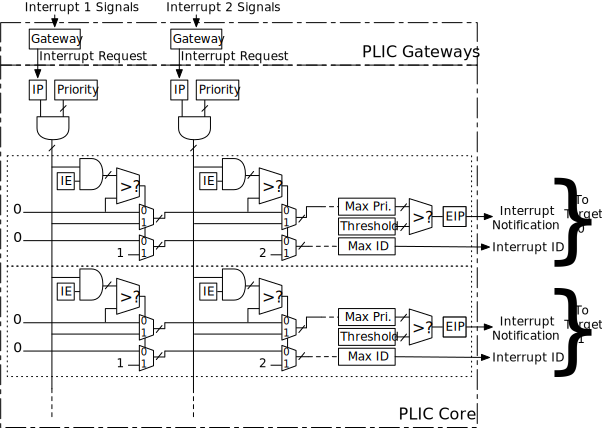
\includegraphics[width=\textwidth]{figs/PLIC-block-diagram.pdf}
\caption{Platform-Level Interrupt Controller (PLIC) conceptual block
  diagram.  The figure shows the first two of potentially many
  interrupt sources, and the first two of potentially many interrupt
  targets.  The figure is just intended to show the logic of the
  PLIC's operation, not to represent a realistic implementation
  strategy.}
\label{fig:plic}
\end{figure}

\section{Interrupt Sources}

RISC-V harts can have both local and global interrupt sources.  Only
global interrupt sources are handled by the PLIC.

\subsection{Local Interrupt Sources}

Each hart has a number of {\em local interrupt sources} that do not
pass through the PLIC, including the standard software interrupts and
timer interrupts for each privilege level.  Local interrupts can be
serviced quickly since there will be minimal latency between the
source and the servicing hart, no arbitration is required to determine
which hart will service the request, and the servicing hart can
quickly determine the interrupt source using the {\tt mcause}
register.

All local interrupts follow a level-based model, where an interrupt is
pending if the corresponding bit in {\tt mip} is set.  The interrupt
handler must clear the hardware condition that is causing the {\tt
  mip} bit to be set to avoid retaking the interrupt after re-enabling
interrupts on exit from the interrupt handler.

Additional platform-specific local interrupt sources can be made visible to
machine-mode by adding them to the high bits of the {\tt mip}/{\tt
  mie} registers, with corresponding additional cause values returned
in the {\tt mcause} register.  These additional platform-specific local
interrupts may also be made visible to lower privilege levels, using
the corresponding bits in the {\tt mideleg} register.  The priority of
these additional interrupt sources relative to external, timer, and
software interrupts is platform-specific.

\subsection{Global Interrupt Sources}

{\em Global interrupt sources} are those that are prioritized and
distributed by the PLIC.  Depending on the platform-specific PLIC
implementation, any global interrupt source could be routed to any
hart context.

Global interrupt sources can take many forms, including
level-triggered, edge-triggered, and message-signalled.  Some sources
might queue up a number of interrupt requests.  All global interrupt
sources are converted to a common interrupt request format for the
PLIC.

\section{Interrupt Targets and Hart Contexts}

Interrupt targets are usually hart contexts, where a hart context is a
given privilege mode on a given hart (though there are other possible
interrupt targets, such as DMA engines).  Not all hart contexts need
be interrupt targets, in particular, if a processor core does not
support delegating external interrupts to lower-privilege modes, then
the lower-privilege hart contexts will not be interrupt targets.
Interrupt notifications generated by the PLIC appear in the {\tt
  meip}/{\tt seip}/{\tt ueip} bits of the {\tt mip}/{\tt sip}/{\tt
  uip} registers for M/S/U modes, respectively.  For the notifications
to appear in lower-privilege {\em x}{\tt ip} registers, the corresponding
external interrupts must have been delegated in the higher-privilege
{\em y}{\tt ideleg} registers.

Each processor core must define a policy on how simultaneous active
interrupts are taken by multiple hart contexts on the core. For the
simple case of a single stack of hart contexts, one for each supported
privileged mode, interrupts for higher-privilege contexts can preempt
execution of interrupt handlers for lower-privilege contexts.  A
multithreaded processor core could run multiple independent interrupt
handlers on different hart contexts at the same time.  A processor
core could also provide hart contexts that are only used for interrupt
handling to reduce interrupt service latency, and these might preempt
interrupt handlers for other harts on the same core.

The PLIC treats each interrupt target independently and does not take
into account any interrupt prioritization scheme used by a component
that contains multiple interrupt targets.  As a result, the PLIC
provides no concept of interrupt preemption or nesting so this must be
handled by the cores hosting multiple interrupt target contexts.

\section{Interrupt Gateways}

The interrupt gateways are responsible for converting global interrupt
signals into a common interrupt request format, and for controlling
the flow of interrupt requests to the PLIC core.  At most one
interrupt request per interrupt source can be pending in the PLIC core
at any time, indicated by setting the source's IP bit.  The gateway
only forwards a new interrupt request to the PLIC core after receiving
notification that the interrupt handler servicing the previous
interrupt request from the same source has completed.

If the global interrupt source uses level-sensitive interrupts, the
gateway will convert the first assertion of the interrupt level into
an interrupt request, but thereafter the gateway will not forward an
additional interrupt request until it receives an interrupt completion
message.  On receiving an interrupt completion message, if the
interrupt is level-triggered and the interrupt is still asserted, a
new interrupt request will be forwarded to the PLIC core.  The gateway
does not have the facility to retract an interrupt request once
forwarded to the PLIC core.  If a level-sensitive interrupt source
deasserts the interrupt after the PLIC core accepts the request and
before the interrupt is serviced, the interrupt request remains
present in the IP bit of the PLIC core and will be serviced by a
handler, which will then have to determine that the interrupt device
no longer requires service.

If the global interrupt source was edge-triggered, the gateway will
convert the first matching signal edge into an interrupt request.
Depending on the design of the device and the interrupt handler,
between sending an interrupt request and receiving notice of its
handler's completion, the gateway might either ignore additional
matching edges or increment a counter of pending interrupts.  In
either case, the next interrupt request will not be forwarded to the
PLIC core until the previous completion message has been received.  If
the gateway has a pending interrupt counter, the counter will be
decremented when the interrupt request is accepted by the PLIC core.

Unlike dedicated-wire interrupt signals, message-signalled interrupts
(MSIs) are sent over the system interconnect via a message packet that
describes which interrupt is being asserted.  The message is decoded
to select an interrupt gateway, and the relevant gateway then handles
the MSI similar to an edge-triggered interrupt.

\section{Interrupt Identifiers (IDs)}

Global interrupt sources are assigned small unsigned integer
identifiers, beginning at the value 1.  An interrupt ID of 0 is
reserved to mean ``no interrupt''.

Interrupt identifiers are also used to break ties when two or more
interrupt sources have the same assigned priority.  Smaller values of
interrupt ID take precedence over larger values of interrupt ID.

\section{Interrupt Priorities}

Interrupt priorities are small unsigned integers, with a
platform-specific maximum number of supported levels.  The priority
value 0 is reserved to mean ``never interrupt'', and interrupt
priority increases with increasing integer values.

Each global interrupt source has an associated interrupt priority held
in a platform-specific memory-mapped register.  Different interrupt
sources need not support the same set of priority values.  A valid
implementation can hardwire all input priority levels.  Interrupt
source priority registers should be \warl\ fields to allow software to
determine the number and position of read-write bits in each priority
specification, if any.  To simplify discovery of supported priority
values, each priority register must support any combination of values
in the bits that are variable within the register, i.e., if there are
two variable bits in the register, all four combinations of values in
those bits must operate as valid priority levels.

\begin{commentary}
 In the degenerate case, all priorities can be hardwired to the value
 1, in which case input priorities are effectively determined by
 interrupt ID.

 The supported priority values can be determined as follows: 1) write
 all zeros to the priority register then 2) read back the value.  Any
 set bits are hardwired to 1.  Next, 3) write all ones to the
 register, and 4) read back the value.  Any clear bits are hardwired
 to 0.  Any set bits that were not found to be hardwired in step 2 are
 variable.  The supported priority levels are the set of values
 obtained by substituting all combinations of ones and zeros in the
 variable bits within the priority field.
\end{commentary}

\section{Interrupt Enables}

Each target has a vector of interrupt enable (IE) bits, one per
interrupt source.  The target will not receive interrupts from sources
that are disabled.  The IE bits for a single target should be packed
together as a bit vector in platform-specific memory-mapped control
registers to support rapid context switching of the IE bits for a
target.  IE bits are \warl\ fields that can be hardwired to either 0
or 1.

\begin{commentary}
A large number of potential IE bits might be hardwired to zero in
cases where some interrupt sources can only be routed to
a subset of targets.

A larger number of bits might be wired to 1 for an embedded device
with fixed interrupt routing.  Interrupt priorities, thresholds, and
hart-internal interrupt masking provide considerable flexibility in
ignoring external interrupts even if a global interrupt source is
always enabled.
\end{commentary}

\section{Interrupt Priority Thresholds}

Each interrupt target has an associated priority threshold, held in a
platform-specific memory-mapped register.  Only active interrupts that
have a priority strictly greater than the threshold will cause a
interrupt notification to be sent to the target.  Different interrupt
targets need not support the same set of priority threshold values.
Interrupt target threshold registers should be \warl\ fields to allow
software to determine the supported thresholds.  A threshold register
should always be able to hold the value zero, in which case, no
interrupts are masked.  If implemented, the threshold register will
usually also be able to hold the maximum priority level, in which case
all interrupts are masked.

\begin{commentary}
A simple valid implementation is to hardwire the threshold to zero, in
which case it has no effect, and the individual enable bits will have
to be saved and restored to attain the same effect.  While the
function of the threshold can be achieved by changing the
interrupt-enable bits, manipulating a single threshold value avoids
the target having to consider the individual priority levels of each
interrupt source, and saving and restoring all the interrupt enables.
Changing the threshold quickly might be especially important for
systems that move frequently between power states.
\end{commentary}

\section{Interrupt Notifications}

Each interrupt target has an {\em external interrupt pending} (EIP)
bit in the PLIC core that indicates that the corresponding target has
a pending interrupt waiting for service.  The value in EIP can change
as a result of changes to state in the PLIC core, brought on by
interrupt sources, interrupt targets, or other agents manipulating
register values in the PLIC.  The value in EIP is communicated to the
destination target as an interrupt notification.  If the target is a
RISC-V hart context, the interrupt notifications arrive on the {\tt
  meip}/{\tt seip}/{\tt ueip} bits depending on the
privilege level of the hart context.

\begin{commentary}
In simple systems, the interrupt notifications will be simple wires
connected to the processor implementing a hart.  In more complex
platforms, the notifications might be routed as messages across a
system interconnect.
\end{commentary}

The PLIC hardware only supports multicasting of interrupts, such that
all enabled targets will receive interrupt notifications for a given
active interrupt.

\begin{commentary}
Multicasting provides rapid response since the fastest responder
claims the interrupt, but can be wasteful in high-interrupt-rate
scenarios if multiple harts take a trap for an interrupt that only one
can successfully claim.  Software can modulate the PLIC IE bits as
part of each interrupt handler to provide alternate policies, such as
interrupt affinity or round-robin unicasting.
\end{commentary}

Depending on the platform architecture and the method used to
transport interrupt notifications, these might take some time to be
received at the targets.  The PLIC is guaranteed to eventually deliver
all state changes in EIP to all targets, provided there is no
intervening activity in the PLIC core.

\begin{commentary}
The value in an interrupt notification is only guaranteed to hold an
EIP value that was valid at some point in the past.  In particular, a
second target can respond and claim an interrupt while a notification
to the first target is still in flight, such that when the first
target tries to claim the interrupt it finds it has no active
interrupts in the PLIC core.
\end{commentary}

\section{Interrupt Claims}

Sometime after a target receives an interrupt notification, it might
decide to service the interrupt.  The target sends an {\em interrupt
  claim} message to the PLIC core, which will usually be implemented
as a non-idempotent memory-mapped I/O control register read.  On
receiving a claim message, the PLIC core will atomically determine the
ID of the highest-priority pending interrupt for the target and then
clear down the corresponding source's IP bit.  The PLIC core will then
return the ID to the target.  The PLIC core will return an ID of zero,
if there were no pending interrupts for the target when the claim was
serviced.

After the highest-priority pending interrupt is claimed by a target
and the corresponding IP bit is cleared, other lower-priority pending
interrupts might then become visible to the target, and so the PLIC
EIP bit might not be cleared after a claim.  The interrupt handler
can check the local {\tt meip}/{\tt seip}/{\tt ueip} bits
before exiting the handler, to allow more efficient service of other
interrupts without first restoring the interrupted context and taking
another interrupt trap.

It is always legal for a hart to perform a claim even if the EIP is
not set.  In particular, a hart could set the threshold value to maximum
to disable interrupt notifications and instead poll for active
interrupts using periodic claim requests, though a simpler approach to
implement polling would be to clear the external interrupt enable in
the corresponding {\em x}{\tt ie} register for privilege mode {\em x}.

\section{Interrupt Completion}

After a handler has completed service of an interrupt, the associated
gateway must be sent an interrupt completion message, usually as a
write to a non-idempotent memory-mapped I/O control register.  The
gateway will only forward additional interrupts to the PLIC core after
receiving the completion message.

\section{Interrupt Flow}

Figure~\ref{fig:intflow} shows the messages flowing between agents
when handling interrupts via the PLIC.

\begin{figure}[hb!]
\centering

\includegraphics[width=4.0in]{figs/PLIC-interrupt-flow.pdf}
\caption{ Flow of interrupt processing via the PLIC.}
\label{fig:intflow}
\end{figure}

The gateway will only forward a single interrupt request at a time to
the PLIC, and not forward subsequent interrupts requests until an
interrupt completion is received.  The PLIC will set the IP bit once
it accepts an interrupt request from the gateway, and sometime later
forward an interrupt notification to the target.  The target might
take a while to respond to a new interrupt arriving, but will then
send an interrupt claim request to the PLIC core to obtain the
interrupt ID.  The PLIC core will atomically return the ID and clear
the corresponding IP bit, after which no other target can claim the
same interrupt request.  Once the handler has processed the interrupt,
it sends an interrupt completion message to the gateway to allow a new
interrupt request.

\section{PLIC Core Specification}

The operation of the PLIC core can be specified as a non-deterministic
finite-state machine with input and output message queues, with the
following atomic actions:

\begin{itemize}

\item {\bf Write Register: } A message containing a register write
  request is dequeued.  One of the internal registers is written,
  where an internal register can be a priority, an interrupt-enable
  (IE), or a threshold.

\item {\bf Accept Request: } If the IP bit corresponding to the
  interrupt source is clear, a message containing an interrupt request
  from a gateway is dequeued and the IP bit is set.

\item {\bf Process Claim: } An interrupt claim message is dequeued.  A
  claim-response message is enqueued to the requester with the ID of
  the highest-priority active interrupt for that target, and the IP
  bit corresponding to this interrupt source is cleared.

\end{itemize}

The value in the EIP bit is determined as a combinational function of
the PLIC Core state.  Interrupt notifications are sent via an
autonomous process that ensures the EIP value is eventually reflected
at the target. 

Note that the operation of the interrupt gateways is decoupled from
the PLIC core.  A gateway can handle parsing of interrupt signals and
processing interrupt completion messages concurrently with other
operations in the PLIC core.

\begin{commentary}
Figure~\ref{fig:plic} is a high-level conceptual view of the PLIC
design.  The PLIC core can be implemented in many ways provided its
behavior can always be understood as following from some sequential
ordering of these atomic actions.  In particular, the PLIC might
process multiple actions in a single clock cycle, or might process
each action over many clock cycles.
\end{commentary}

\section{Controlling Access to the PLIC}

In the expected use case, only machine mode accesses the source
priority, source pending, and target interrupt enables to configure
the interrupt subsystem.  Lower-privilege modes access these features
via ABI or SBI calls. The interrupt enables act as a protection
mechanism where a target can only signal completion to an interrupt
gateway that is currently enabled for that target.

Interrupt handlers that run with lower than machine-mode privilege
need only be able to perform a claim read and a completion write, and
to set their target threshold value.  The memory map for these
registers should allow machine mode to protect different targets from
each other's accesses, using either physical memory protection or
virtual memory page protections.


\chapter{Machine Configuration Description}
\label{cfgstr}

\begin{commentary}
  To reduce porting effort for OS boots, we have reverted back to
  using Device Trees to communicate platform information to the
  kernel, so this chapter is out of date.  Config string was designed
  for other uses in addition, but for now, we are staying with a
  standard device tree model.
 \end{commentary}

RISC-V platforms may contain myriad devices, processor cores, and
configuration parameters.  To support higher-level software, including
bootloaders and operating systems, it is recommended that hardware
platforms embed a description of their components in read-only memory
that is directly accessible after processor reset for use by low-level
system software, external debuggers, or manufacturing test procedures.
We call this low-level embedded information a configuration
description.  We define here a standard mechanism to encode and locate
the configuration information, and to determine the format of the
configuration information.

\section{Configuration String Search Procedure}

The platform must describe how to locate a pointer to find this
string, for example, by specifying a fixed physical address at which
the pointer resides.  To support a wide variety of platforms,
configuration formats, and chips with manufacturing-time programming
of configuration options, a flexible search procedure is defined to
locate the configuration information seeded by the initial pointer
specified by the platform.

The configuration string pointer provided by the platform points to an
initial memory address at which the search for configuration string
begins.

The configuration string cannot begin with a padding byte, where a
padding byte is defined to contain either {\tt 0x0} or {\tt 0xff}, but
can be preceded by up to 63 padding bytes that are ignored.  If 64
padding bytes are encountered, then the search terminates without
finding a config string.

\begin{commentary}
The padding bytes represent common values returned by unpopulated
memory or bus regions or unprogrammed non-volatile
memory. Configuration strings can therefore include pointers to
regions that are optionally populated or programmed, and these regions
will be ignored if there is nothing present.  The padding bytes also
support alignment of binary data structures.
\end{commentary}

Otherwise the first non-padding byte is the beginning of the
configuration information.  For example, configuration information in
Device Tree String format would begin with a ``/dts-v1/''.
Configuration information in Flattened Device Tree format would begin
with the magic number {\tt 0xd00dfeed}.  Configuration information in
the config string format would begin with ``/cs-v1/''.
\begin{commentary}
  Config string is a new format that is backwards-compatible with
  device tree string (as far as DTS specs exist) but can include
  additional configuration information in other memory regions.
\end{commentary}


\chapter{Supervisor Binary Interface (SBI)}

This chapter is a placeholder to describe the form of the SBIs we're
envisioning for the RISC-V supervisor.

The SBI captures the instructions that can be executed together with a
set of SBI calls out to the supervisor execution environment (SEE) on
a given platform.

Several features that might normally handled by the supervisor
operating system (OS) directly are handled via SBI calls to the SEE in
RISC-V, including:

\begin{itemize}

\item Reset is handled by the SEE and once the machine is set up, the
  OS kernel is mapped into virtual memory, and its entry point is called.

\item Machine-check errors and other non-maskable interrupts are
  handled by the SEE before vectoring into the OS if recovery is
  possible.

\item Some device drivers may be handled by the SEE, and managed via
  virtual device calls over the SBI.

\item The presence and version of supported instruction-set extensions
  is obtained via an SBI call to return the configuration string
  rather than a machine register.  This allows for an arbitrarily
  large definition of instruction set extensions, and simplifies
  virtualization where the returned machine configuration might be
  modified to emulate different architectures on a given hardware
  platform.

\end{itemize}

The SBI employs the same calling convention as the ABI specified in Volume
I of this manual.  SBI entry points are located in the uppermost
\wunits{2}{KiB} of the virtual address space, so that they may be invoked with
a single {\tt jalr} instruction with {\tt x0} as the base register.

Table~\ref{sbicalls} gives a preliminary list of SBI calls.

\begin{table*}[h!]
\begin{center}
\begin{tabular}{| >{\ttfamily\catcode`_=12}l|p{8cm}|}
\hline
const char* sbi_get_config(void); & \parbox{8cm}{Get pointer to
  configuration string.}\\ \hline
size_t sbi_hart_id(void); & \parbox{8cm}{Get ID of current hart, in
  range \\ {\tt [0, number\_harts - 1 ]}.} \\ \hline
int sbi_send_ipi(size_t hart_id); & Send an interprocessor interrupt; returns 0 on success or -1 if hart ID is invalid. \\ \hline
bool sbi_clear_ipi(void); & Clear local interprocessor interrupt. Returns 1 if an IPI was pending, else 0. \\ \hline
void sbi_shutdown(void); & Terminate this supervisor-mode process. \\ \hline
int sbi_console_putchar(uint8_t ch); & Write byte to debug console (blocking); returns 0 on success, else -1. \\ \hline
int sbi_console_getchar(void); & Read byte from debug console; returns the byte on success, or -1 for failure. \\ \hline

& \multirow{4}{*}{\parbox{8cm}{Instruct other harts to execute SFENCE.VMA.  {\tt harts} points to a bitmask of remote hart IDs; NULL indicates all harts.  {\tt asid} holds the address-space ID; 0 indicates all address spaces.}} \\
void sbi_remote_sfence_vm( & \\
\ \ const uintptr_t* harts, size_t asid); & \\
& \\ \hline

void sbi_remote_sfence_vm_range(
& \multirow{3}{*}{\parbox{8cm}{Like {\tt sbi\_remote\_sfence\_vm}, but only orders updates to leaf page tables mapping the range {\tt [start, start+size-1]}.}} \\
\ \ const uintptr_t* harts, size_t asid, & \\
\ \ uintptr_t start, uintptr_t size); & \\ \hline

void sbi_remote_fence_i(
& \multirow{2}{*}{\parbox{8cm}{Instruct remote harts to execute FENCE.I.  {\tt harts} is as with {\tt sbi\_remote\_sfence\_vm}.}} \\
\ \ const uintptr_t* harts); & \\ \hline

int sbi_mask_interrupt(int which); & Disable a PLIC interrupt line. Returns 0 if previously disabled, 1 if previously enabled, or -1 if {\tt which} is invalid. \\ \hline
int sbi_unmask_interrupt(int which); & Enable a PLIC interrupt line. Return value is as with {\tt sbi\_mask\_interrupt}. \\ \hline
\end{tabular}
\end{center}
\caption{SBI calls.}
\label{sbicalls}
\end{table*}

\input{priv-history}

\bibliographystyle{plain}
\bibliography{riscv-spec}

\end{document}
